


\chapter{Notion de fonction}

\section{Généralités sur les fonctions}

\subsection{Vocabulaire}

\subsubsection{Définition et exemples}

\begin{Définition} 
Soit $D$ une partie de l'ensemble des réels $\R$. Définir une fonction sur $D$, c'est associer à chaque réel $x$ de $D$ un UNIQUE nombre réel, noté $f(x)$. \\
$D$ est appelé domaine de définition de $f$.
\end{Définition}

\begin{Notation}
On notera $f : x \mapsto f(x)$ pour la fonction qui à $x$ associe $f(x)$.
\end{Notation}

\begin{Exemple} 
\begin{minipage}[c]{0.7\textwidth}


On considère $D = \left\lbrace  -1,2; 3; 0; \dfrac{7}{3} \right\rbrace$.

Résumé des informations d'une fonction $f$ dans un tableau :
\end{minipage} \hfill \begin{minipage}[c]{0.3\textwidth}
\begin{center}
\begin{tabular}{|c|c|c|c|c|}
\hline
$x$ & -1,2 & 3 & 0 & $\dfrac{7}{3}$ \\
\hline
$f(x)$ & 4 & 7 & $\pi$ & 7 \\
\hline
\end{tabular}
\end{center}
\end{minipage} \\

$f$ est bien une fonction car chaque réel de $D$ est associé à un unique réel de $\R$. \\
On a ainsi \ligne

\end{Exemple}

\subsubsection{Image, antécédents}

\begin{Définition} 
Soit $f$ une fonction définie sur un domaine de définition $D$. Soit $x \in D$.

\begin{itemize}[label=\textcolor{Couleur6}{$\bullet$}]
    \item On dit que $f(x)$ est \textbf{l'}image de $x$ par $f$.
    \item On dit que $x$ est \textbf{un} antécédent de $f(x)$ par $f$.
\end{itemize}
\end{Définition}

L'antécédent doit TOUJOURS appartenir au domaine de définition !
\vspace{0.5cm}
\begin{Remarque}
Attention un nombre peut avoir plusieurs antécédents mais ne peut avoir qu'une UNIQUE image.
\end{Remarque}
\vspace{0.5cm}
\begin{Exemple}
\vspace{0.1cm} 
\ligne

\ligne

\end{Exemple}

\begin{Exemple}
On considère la fonction $g$ définie par $g(x) = 2x + 3$ sur $\R$.
\vspace{0.1cm} 
\ligne

\ligne

\ligne

\ligne

\ligne

\ligne

\end{Exemple}

\newpage

\section{Représentation graphique}

Dans toute la suite, on se place dans un repère $(O, \overrightarrow{i}, \overrightarrow{j})$ orthonormé.

\subsection{Courbe représentative}

\begin{Définition}
Soit $f$ une fonction et $D$ son domaine de définition. On appelle représentation graphique de $f$ (ou courbe représentative de $f$) l'ensemble des points $M$ de coordonnées $(x, f(x))$, pour tout $x \in D$. On note en général cette courbe $C_f$.
\end{Définition}

\begin{Exemple}
On trace la représentation graphique d'une certaine fonction $h$.

\begin{center}
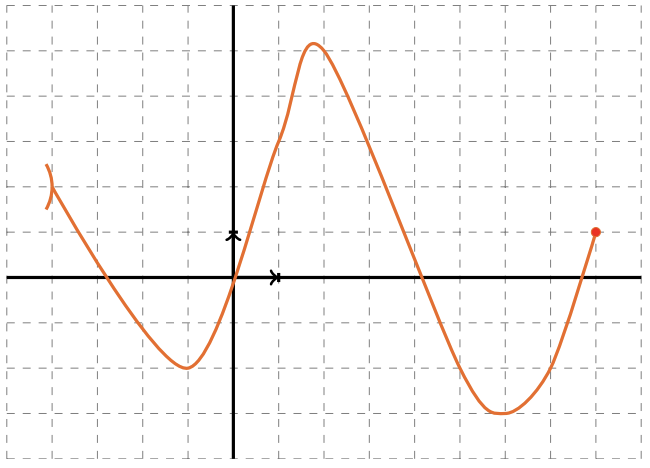
\includegraphics[scale=.7]{Ch 2/Ex5}
\end{center}

\begin{itemize}[label=\textcolor{Couleur10}{$\bullet$}]
    \item Le domaine de définition de $h$ est \pointille{3cm}
    \item Le point de coordonnées $(-1, -2)$ est sur la courbe, ce qui signifie que \pointille{3cm}
    \item L'image de $1$ par $h$ est \pointille{3cm}
    \item $-2$ a \pointille{2cm} antécédents par $h$ : \pointille{4cm}. Et $6$ \pointille{6cm}
\end{itemize}
\end{Exemple}

\subsection{Résolutions graphiques}

\textbf{Équation $f(x) = k$ ou inéquation $f(x) > k$}

\begin{Exemple}
Soit $f$ définie sur $I = [-4, 2]$ par $f(x) = x^2 + 2x - 1$. 

\begin{minipage}{0.35\linewidth}
\begin{center}
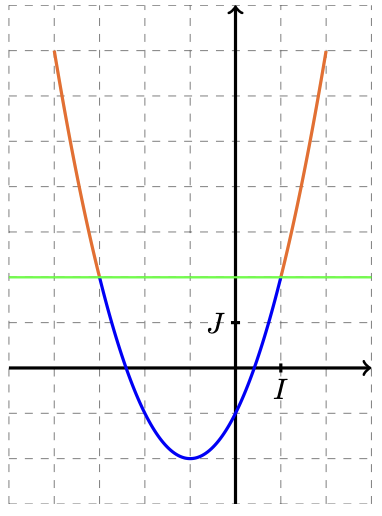
\includegraphics[scale=.65]{Ch 2/Ex6}
\end{center}
\end{minipage}
\begin{minipage}{0.6\linewidth}
On donne la courbe représentative de $f$ ci-contre.

Pour résoudre l'équation $f(x) = 2$ sur $I$, c'est-à-dire déterminer les antécédents de $2$ par $f$, on regarde les points de la courbe dont l'ordonnée vaut $2$. Les antécédents de $2$ par $f$ sont \pointille{2cm}. Les solutions de $x^2 + 2x - 1 = 2$ sur $I$ sont donc \pointille{2cm}

Résoudre l'inéquation $f(x) > 2$ sur $I$ revient à déterminer l'ensemble des abscisses des points de la courbe représentative de $f$ dont l'ordonnée est supérieure ou égale à $2$. Dans notre cas, l'ensemble des solutions est \pointille{4cm}
\end{minipage}
\end{Exemple}

\newpage

\textbf{Équation $f(x) = g(x)$ ou inéquation $f(x) \leq g(x)$}

\begin{Exemple} 
\begin{minipage}{0.3\linewidth}
\begin{center}

\includegraphics[scale=.6]{Ch 2/Ex7}
\end{center}
\end{minipage}
\begin{minipage}{0.6\linewidth}
Soit $f$ et $g$ définies sur $I = [-2; 6]$ par $f(x) = x^2 - 5x - 3$ et $g(x) = -2x - 1$. On donne les courbes représentatives de $f$ et $g$ ci-contre. 

Pour résoudre l'équation $f(x) = g(x)$ sur $I$, on cherche les $x$ correspondants aux points d'intersection des courbes représentatives de ces deux fonctions. 

Ici, les courbes se croisent pour \pointille{4cm} Les solutions de $f(x) = g(x)$, c'est-à-dire $x^2 - 5x - 3 = -2x - 1$ sur $I$ sont donc \pointille{2cm} 

Résoudre l'inéquation $f(x) > g(x)$ sur $I$ revient à déterminer l'ensemble des abscisses pour lesquelles la courbe de $f$ est au-dessus de celle de $g$. 

Dans notre cas, l'ensemble des solutions est \pointille{4cm}
\end{minipage}
\end{Exemple}

\section{Variations d'une fonction}

\begin{Définition}
Soit $f$ une fonction définie sur un intervalle $I$.
\begin{itemize}[label=\textcolor{Couleur6}{$\bullet$}]
    \item On dit que $f$ est croissante lorsque, pour tout $a$ et $b$ dans $I$, si $a < b$, alors $f(a) \leq f(b)$. \\
    Autrement dit, $f$ conserve l'ordre sur $I$.
    \item On dit que $f$ est décroissante lorsque, pour tout $a$ et $b$ dans $I$, si $a < b$, alors $f(a) \geq f(b)$. \\
    Autrement dit, $f$ renverse l'ordre sur $I$.
\end{itemize}
\end{Définition}

\begin{Remarque}
Si les inégalités sont strictes, on parlera de fonction strictement croissante ou décroissante.
\end{Remarque}

\begin{Définition} 
Avec les mêmes notations, on dit que $f$ est constante sur $I$ si, pour tout $a$ et $b$ dans $I$, on a $f(a) = f(b)$.
\end{Définition}

\subsection{Interprétation graphique}

Si la fonction est croissante sur un intervalle $I$, sa courbe représentative "monte" de gauche à droite. Si la fonction est décroissante, la courbe descend. 

Si la courbe est horizontale, la fonction est constante sur l'intervalle correspondant.

\begin{Exemple} 
\begin{minipage}[c]{.5\textwidth}

On considère une fonction $f$ dont la courbe représentative est donnée ci-dessous.

\begin{center}

\includegraphics[scale=.6]{Ch 2/Ex8}
\end{center}
\end{minipage} \hfill \begin{minipage}[c]{.5\textwidth}

Le domaine de définition de $f$ est \pointille{2cm}

$f$ est croissante sur \pointille{2cm}, puis décroissante sur \pointille{2cm}, puis constante sur\pointille{2cm}, puis croissante sur \pointille{2cm}, puis décroissante sur \pointille{2cm}
\end{minipage} 

\end{Exemple}

\newpage

\subsection{Tableau de variation}

On peut résumer les variations d'une fonction $f$ dans un tableau de variations. Pour la courbe donnée précédemment, le tableau de variations se présente ainsi :

\begin{center}
\begin{tikzpicture}[scale=.6]
   \tkzTabInit{$x$ / 1 , $f(x)$ / 2}{$-4$, $-2$, $1$, $4$, $5$, $ 6 $}
   \tkzTabVar{D-/$ 2 $ , +/ $4$, -/ $3$, -/ $3$, +/ $4$, -/ $2$}
\end{tikzpicture}
\end{center}

La double barre en -4 traduit le fait que -4 n'est pas dans l'ensemble de définition.

\begin{Exemple}

On considère une fonction $f$ dont le tableau de variations est le suivant : \\
 \begin{minipage}[c]{.45\textwidth}
\begin{center}
\begin{tikzpicture}[scale=.7]
   \tkzTabInit{$x$ / 1 , $f(x)$ / 2}{$-4$, $0$, $2$, $5$}
   \tkzTabVar{+/ $2$, -/ $-1$, +/ $0$, -/ $-2$}
\end{tikzpicture}
\end{center}
\end{minipage} \hfill \begin{minipage}[c]{.5\textwidth}
$ $ \\
\begin{itemize}[label=\textcolor{Couleur10}{$\bullet$}]
    \item Le domaine de définition se lit sur la première ligne : \pointille{2cm}
    \item \ligne
    \item On souhaite encadrer $f(1)$. On sait que $1 \in$\pointille{2cm} et $f$ est \pointille{2cm} sur cet intervalle.
    \ligne
    
    \ligne
    
\end{itemize}
\end{minipage}

\end{Exemple}

\section{Signe d'une fonction}

\begin{Remarque}
Il est également possible de faire un tableau de signes pour une fonction. Lorsque la fonction est définie par une expression algébrique, on peut procéder comme au chapitre précédent. Graphiquement, cela revient à donner la position relative de la courbe par rapport à l'axe des abscisses.
\end{Remarque}

\begin{Exemple}
On considère la fonction $f$ définie sur $\R$ et dont la courbe représentative dans un repère orthonormé est donnée ci-dessous.
\vspace{-0.5cm}
\begin{center}
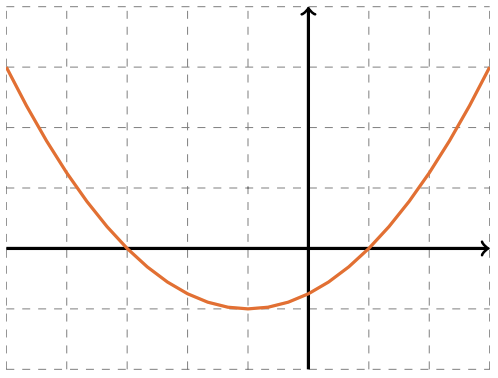
\includegraphics[scale=.65]{Ch 2/Ex10}
\end{center}

\vspace{4cm}
\end{Exemple}
\newpage
\section{Extremum}

\begin{Définition}
Soit $f$ une fonction définie sur un intervalle $I$ et $a \in I$ :
\begin{itemize}[label=\textcolor{Couleur6}{$\bullet$}]
    \item On dit que $f$ admet un minimum en $a$ sur $I$ si, pour tout $x$ dans $I$, on a $f(a) \leq f(x)$.
    \item On dit que $f$ admet un maximum en $a$ sur $I$ si, pour tout $x$ dans $I$, on a $f(a) \geq f(x)$.
    \item On dit que $f$ admet un extremum en $a$ si $f$ admet un minimum ou un maximum en $a$.
\end{itemize}
\end{Définition}

\begin{Exemple}

On considère une fonction $f$ dont la représentation graphique est donnée ci-dessous :\\
\begin{minipage}[c]{.4\textwidth}
\begin{center}

\includegraphics[scale=.55]{Ch 2/Ex11}
\end{center}
\end{minipage} \hfill \begin{minipage}[c]{.6\textwidth}
\begin{itemize}[label=\textcolor{Couleur10}{$\bullet$}]
    \item Le domaine de définition de $f$ est \pointille{2cm}
    \item Le maximum de $f$ sur $D$ \ligne
    \item Le minimum de $f$ sur $D$ \ligne
    \item Le maximum de $f$ sur $[0; 4]$ \ligne
\end{itemize}
\end{minipage}

\end{Exemple}

\section{Parité, Imparité}

\begin{Définition*}
Soit $D$ une partie de $\R$. On dit que $D$ est symétrique par rapport à $0$ si, pour tout $x \in D$, $-x \in D$.
\end{Définition*}

\begin{Exemple}
$[-1; 1]$ est symétrique par rapport à $0$. $[-3; 4]$ ne l'est pas. En effet, \ligne

\end{Exemple}

\begin{Définition}
Soit $D$ une partie de $\R$ symétrique par rapport à $0$ et $f$ une fonction définie sur $D$.
\begin{itemize}[label=\textcolor{Couleur6}{$\bullet$}]
    \item On dit que $f$ est paire si, pour tout $x \in D$, $f(-x) = f(x)$.
    \item On dit que $f$ est impaire si, pour tout $x \in D$, $f(-x) = -f(x)$.
\end{itemize}
\end{Définition}

\begin{Exemple}
La fonction $f : x \mapsto x^2 - 2$, définie sur $\R$ est \pointille{2cm} \\

\ligne

\end{Exemple}

\newpage

\begin{Propriété}
Soit $f$ une fonction et $C_f$ sa courbe représentative dans un repère orthogonal.
\begin{itemize}[label=\textcolor{Couleur2}{$\bullet$}]
    \item $f$ est paire si et seulement si $C_f$ est symétrique par rapport à l'axe des ordonnées.
    \item $f$ est impaire si et seulement si $C_f$ est symétrique par rapport à l'origine du repère.
\end{itemize}
\end{Propriété}

\begin{Exemple}
\begin{minipage}[t]{0.45\linewidth}
Courbe représentative d'une fonction \pointille{2cm} \\
\begin{center}
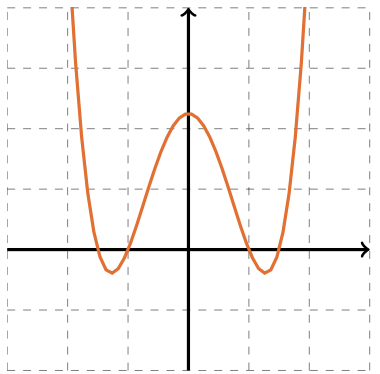
\includegraphics[scale=.9]{Ch 2/Ex14_1}
\end{center}
\end{minipage}
\begin{minipage}[t]{0.45\linewidth}
Courbe représentative d'une fonction \pointille{2cm} \\
\begin{center}
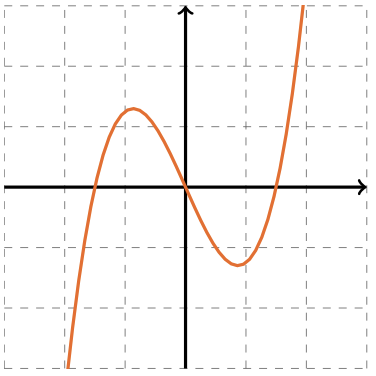
\includegraphics[scale=.9]{Ch 2/Ex14 Bis}
\end{center}
\end{minipage}

\end{Exemple}

\bigskip

\newpage

\section*{Exercices - Notion de fonction}
\addcontentsline{toc}{section}{Exercices}
{\setlength{\columnseprule}{0pt}
\setcounter{NumEx}{1}

\subsection*{Vocabulaire}


\begin{Exercice}%1
On considère une fonction \( f \). Compléter chaque phrase par le mot qui convient.
\begin{enumerate}
    \item Si \( f(4) = -2 \), alors...
    \begin{enumerate}
        \item $ -2 $ est \phantom{l'image} de 4 par la fonction \( f \).
        \item 4 est \phantom{un antécédent} de $ -2 $ par la fonction \( f \).
    \end{enumerate}
    \item Si l'image de $ -6 $ par la fonction est 1, alors...
    \begin{enumerate}
        \item 1 est \phantom{l'image} de $ -6 $ par la fonction \( f \).
        \item \( f(...) = ... \).
    \end{enumerate}
    \item Si un antécédent de 7 par la fonction est 3, alors :
    \begin{enumerate}
        \item 3 est \phantom{un antécédent} de 7 par la fonction \( f \).
        \item \( f(...) = ... \).
    \end{enumerate}
    \item Si \( f(-1) = 3 \), alors...
    \begin{enumerate}
        \item 3 est \phantom{l'image} de $ -1 $ par la fonction \( f \).
        \item $ -1 $ est \phantom{un antécédent} de 3 par la fonction \( f \).
    \end{enumerate}
    \item Si l'image de 5 par la fonction est 3, alors...
    \begin{enumerate}
        \item 5 est \phantom{un antécédent} de 3 par la fonction \( f \).
        \item \( f(...) = ... \).
    \end{enumerate}
    \item Si un antécédent de 8 par la fonction est $ -1 $, alors :
    \begin{enumerate}
        \item $ -1 $ est \phantom{un antécédent} de 8 par la fonction \( f \).
        \item \( f(...) = ... \).
    \end{enumerate}
\end{enumerate}
\vspace{-0.5cm}
\end{Exercice}

\begin{Exercice}%2
On considère une fonction \( f \). Compléter chaque phrase par le mot qui convient.
\begin{enumerate}
    \item Si \( f(3) = -7 \), alors...
    \begin{enumerate}
        \item 3 est \phantom{un antécédent} de $ -7 $ par la fonction \( f \).
        \item $ -7 $ est \phantom{l'image} de 3 par la fonction \( f \).
    \end{enumerate}
    \item Si l'image de 5 par la fonction est $ -3 $, alors...
    \begin{enumerate}
        \item $ -3 $ est \phantom{l'image} de 5 par la fonction \( f \).
        \item \( f(...) = ... \).
    \end{enumerate}
    \item Si un antécédent de $ -4 $ par la fonction est 8, alors :
    \begin{enumerate}
        \item 8 est \phantom{un antécédent} de $ -4 $ par la fonction \( f \).
        \item \( f(...) = ... \).
    \end{enumerate}
    \item Si \( f(...) = ... \), alors...
    \begin{enumerate}
        \item 2 est \phantom{un antécédent} de 9 par la fonction \( f \).
        \item 9 est \phantom{l'image} de 2 par la fonction \( f \).
    \end{enumerate}
    \item Si l'image de $ -4 $ par la fonction est 7, alors...
    \begin{enumerate}
        \item $ -4 $ est \phantom{un antécédent} de 7 par la fonction \( f \).
        \item \( f(...) = ... \).
    \end{enumerate}
\end{enumerate}
\vspace{-0.5cm}
\end{Exercice}

\newpage

\subsection*{Représentation graphique}


\begin{multicols}{2}



% @see : https://coopmaths.fr/alea?uuid=e46e6&id=200F3-02&n=1&d=10&s=1&alea=2s53&cd=1&cols=1
\begin{Exercice}%1

\begin{tikzpicture}[scale=0.65]

    \tikzset{
      point/.style={
        thick,
        draw,
        cross out,
        inner sep=0pt,
        minimum width=5pt,
        minimum height=5pt,
      },
    }

    	
	\draw[color ={black},>=latex,->] (-6,0)--(5,0);
	\draw[color ={black},>=latex,->] (0,-4)--(0,3);
	\draw[color ={black},opacity = 0.4] (-6,1)--(5,1);
	\draw[color ={black},opacity = 0.4] (-6,2)--(5,2);
	\draw[color ={black},opacity = 0.4] (-6,3)--(5,3);
	\draw[color ={black},opacity = 0.4] (-6,-1)--(5,-1);
	\draw[color ={black},opacity = 0.4] (-6,-2)--(5,-2);
	\draw[color ={black},opacity = 0.4] (-6,-3)--(5,-3);
	\draw[color ={black},opacity = 0.4] (-6,-4)--(5,-4);
	\draw[color ={black},opacity = 0.4] (1,-4)--(1,3);
	\draw[color ={black},opacity = 0.4] (2,-4)--(2,3);
	\draw[color ={black},opacity = 0.4] (3,-4)--(3,3);
	\draw[color ={black},opacity = 0.4] (4,-4)--(4,3);
	\draw[color ={black},opacity = 0.4] (5,-4)--(5,3);
	\draw[color ={black},opacity = 0.4] (-1,-4)--(-1,3);
	\draw[color ={black},opacity = 0.4] (-2,-4)--(-2,3);
	\draw[color ={black},opacity = 0.4] (-3,-4)--(-3,3);
	\draw[color ={black},opacity = 0.4] (-4,-4)--(-4,3);
	\draw[color ={black},opacity = 0.4] (-5,-4)--(-5,3);
	\draw[color ={black},opacity = 0.4] (-6,-4)--(-6,3);
	\draw[color ={black},line width = 1.2] (1,-0.13)--(1,0.13);
	\draw[color ={black},line width = 1.2] (2,-0.13)--(2,0.13);
	\draw[color ={black},line width = 1.2] (3,-0.13)--(3,0.13);
	\draw[color ={black},line width = 1.2] (4,-0.13)--(4,0.13);
	\draw[color ={black},line width = 1.2] (-1,-0.13)--(-1,0.13);
	\draw[color ={black},line width = 1.2] (-2,-0.13)--(-2,0.13);
	\draw[color ={black},line width = 1.2] (-3,-0.13)--(-3,0.13);
	\draw[color ={black},line width = 1.2] (-4,-0.13)--(-4,0.13);
	\draw[color ={black},line width = 1.2] (-5,-0.13)--(-5,0.13);
	\draw[color ={black},line width = 1.2] (-0.13,1)--(0.13,1);
	\draw[color ={black},line width = 1.2] (-0.13,2)--(0.13,2);
	\draw[color ={black},line width = 1.2] (-0.13,-1)--(0.13,-1);
	\draw[color ={black},line width = 1.2] (-0.13,-2)--(0.13,-2);
	\draw[color ={black},line width = 1.2] (-0.13,-3)--(0.13,-3);
	\draw (1,-0.4) node[anchor = center] {\scriptsize \color{black}{$1$}};
	\draw (2,-0.4) node[anchor = center] {\scriptsize \color{black}{$2$}};
	\draw (3,-0.4) node[anchor = center] {\scriptsize \color{black}{$3$}};
	\draw (4,-0.4) node[anchor = center] {\scriptsize \color{black}{$4$}};
	\draw (5,-0.4) node[anchor = center] {\scriptsize \color{black}{$5$}};
	\draw (-1,-0.4) node[anchor = center] {\scriptsize \color{black}{$-1$}};
	\draw (-2,-0.4) node[anchor = center] {\scriptsize \color{black}{$-2$}};
	\draw (-3,-0.4) node[anchor = center] {\scriptsize \color{black}{$-3$}};
	\draw (-4,-0.4) node[anchor = center] {\scriptsize \color{black}{$-4$}};
	\draw (-5,-0.4) node[anchor = center] {\scriptsize \color{black}{$-5$}};
	\draw (-6,-0.4) node[anchor = center] {\scriptsize \color{black}{$-6$}};
	\draw (-0.5,1.1) node[anchor = center] {\footnotesize \color{black}{$1$}};
	\draw (-0.5,2.1) node[anchor = center] {\footnotesize \color{black}{$2$}};
	\draw (-0.5,3.1) node[anchor = center] {\footnotesize \color{black}{$3$}};
	\draw (-0.5,-0.9) node[anchor = center] {\footnotesize \color{black}{$-1$}};
	\draw (-0.5,-1.9) node[anchor = center] {\footnotesize \color{black}{$-2$}};
	\draw (-0.5,-2.9) node[anchor = center] {\footnotesize \color{black}{$-3$}};
	\draw (-0.5,-3.9) node[anchor = center] {\footnotesize \color{black}{$-4$}};
	    \clip (-6,-4) rectangle (5,3);
	\draw[color = {Couleur10},line width = 1, opacity = 1](-4,1.5) .. controls +(0.33,-0.67) and +(-0.33,0.00)  .. (-3.00,-1.50)
 .. controls +(0.67,0.00) and +(-0.67,0.00)  .. (-1.00,1.50)
 .. controls +(0.67,0.00) and +(-0.67,0.00)  .. (1.00,1.50)
 .. controls +(0.67,0.00) and +(-0.67,1.33)  .. (3.00,-2.50)
;

	
	 \filldraw[color={Couleur10},fill={black}] (-4,1.5) circle (0.05);
	
	 \filldraw[color={Couleur10},fill={black}] (3,-2.5) circle (0.05);

\end{tikzpicture}\\Quel est l'ensemble de définition de la fonction représentée ci-dessus ?
\end{Exercice}


% @see : https://coopmaths.fr/alea?uuid=e46e6&id=200F3-02&n=1&d=10&s=2&alea=GgFi&cd=1&cols=1
\begin{Exercice}%2
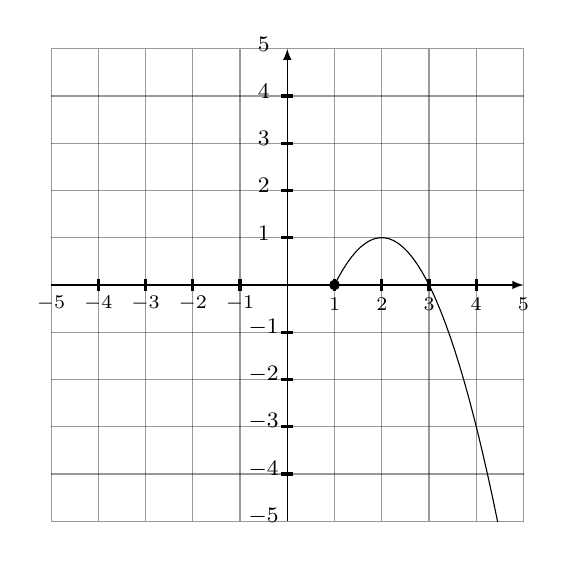
\begin{tikzpicture}[scale=0.6]

    \tikzset{
      point/.style={
        thick,
        draw,
        cross out,
        inner sep=0pt,
        minimum width=5pt,
        minimum height=5pt,
      },
    }

    	
	\draw[color ={black},>=latex,->] (-5,0)--(5,0);
	\draw[color ={black},>=latex,->] (0,-5)--(0,5);
	\draw[color ={black},opacity = 0.4] (-5,1)--(5,1);
	\draw[color ={black},opacity = 0.4] (-5,2)--(5,2);
	\draw[color ={black},opacity = 0.4] (-5,3)--(5,3);
	\draw[color ={black},opacity = 0.4] (-5,4)--(5,4);
	\draw[color ={black},opacity = 0.4] (-5,5)--(5,5);
	\draw[color ={black},opacity = 0.4] (-5,-1)--(5,-1);
	\draw[color ={black},opacity = 0.4] (-5,-2)--(5,-2);
	\draw[color ={black},opacity = 0.4] (-5,-3)--(5,-3);
	\draw[color ={black},opacity = 0.4] (-5,-4)--(5,-4);
	\draw[color ={black},opacity = 0.4] (-5,-5)--(5,-5);
	\draw[color ={black},opacity = 0.4] (1,-5)--(1,5);
	\draw[color ={black},opacity = 0.4] (2,-5)--(2,5);
	\draw[color ={black},opacity = 0.4] (3,-5)--(3,5);
	\draw[color ={black},opacity = 0.4] (4,-5)--(4,5);
	\draw[color ={black},opacity = 0.4] (5,-5)--(5,5);
	\draw[color ={black},opacity = 0.4] (-1,-5)--(-1,5);
	\draw[color ={black},opacity = 0.4] (-2,-5)--(-2,5);
	\draw[color ={black},opacity = 0.4] (-3,-5)--(-3,5);
	\draw[color ={black},opacity = 0.4] (-4,-5)--(-4,5);
	\draw[color ={black},opacity = 0.4] (-5,-5)--(-5,5);
	\draw[color ={black},line width = 1.2] (1,-0.13)--(1,0.13);
	\draw[color ={black},line width = 1.2] (2,-0.13)--(2,0.13);
	\draw[color ={black},line width = 1.2] (3,-0.13)--(3,0.13);
	\draw[color ={black},line width = 1.2] (4,-0.13)--(4,0.13);
	\draw[color ={black},line width = 1.2] (-1,-0.13)--(-1,0.13);
	\draw[color ={black},line width = 1.2] (-2,-0.13)--(-2,0.13);
	\draw[color ={black},line width = 1.2] (-3,-0.13)--(-3,0.13);
	\draw[color ={black},line width = 1.2] (-4,-0.13)--(-4,0.13);
	\draw[color ={black},line width = 1.2] (-0.13,1)--(0.13,1);
	\draw[color ={black},line width = 1.2] (-0.13,2)--(0.13,2);
	\draw[color ={black},line width = 1.2] (-0.13,3)--(0.13,3);
	\draw[color ={black},line width = 1.2] (-0.13,4)--(0.13,4);
	\draw[color ={black},line width = 1.2] (-0.13,-1)--(0.13,-1);
	\draw[color ={black},line width = 1.2] (-0.13,-2)--(0.13,-2);
	\draw[color ={black},line width = 1.2] (-0.13,-3)--(0.13,-3);
	\draw[color ={black},line width = 1.2] (-0.13,-4)--(0.13,-4);
	\draw (1,-0.4) node[anchor = center] {\scriptsize \color{black}{$1$}};
	\draw (2,-0.4) node[anchor = center] {\scriptsize \color{black}{$2$}};
	\draw (3,-0.4) node[anchor = center] {\scriptsize \color{black}{$3$}};
	\draw (4,-0.4) node[anchor = center] {\scriptsize \color{black}{$4$}};
	\draw (5,-0.4) node[anchor = center] {\scriptsize \color{black}{$5$}};
	\draw (-1,-0.4) node[anchor = center] {\scriptsize \color{black}{$-1$}};
	\draw (-2,-0.4) node[anchor = center] {\scriptsize \color{black}{$-2$}};
	\draw (-3,-0.4) node[anchor = center] {\scriptsize \color{black}{$-3$}};
	\draw (-4,-0.4) node[anchor = center] {\scriptsize \color{black}{$-4$}};
	\draw (-5,-0.4) node[anchor = center] {\scriptsize \color{black}{$-5$}};
	\draw (-0.5,1.1) node[anchor = center] {\footnotesize \color{black}{$1$}};
	\draw (-0.5,2.1) node[anchor = center] {\footnotesize \color{black}{$2$}};
	\draw (-0.5,3.1) node[anchor = center] {\footnotesize \color{black}{$3$}};
	\draw (-0.5,4.1) node[anchor = center] {\footnotesize \color{black}{$4$}};
	\draw (-0.5,5.1) node[anchor = center] {\footnotesize \color{black}{$5$}};
	\draw (-0.5,-0.9) node[anchor = center] {\footnotesize \color{black}{$-1$}};
	\draw (-0.5,-1.9) node[anchor = center] {\footnotesize \color{black}{$-2$}};
	\draw (-0.5,-2.9) node[anchor = center] {\footnotesize \color{black}{$-3$}};
	\draw (-0.5,-3.9) node[anchor = center] {\footnotesize \color{black}{$-4$}};
	\draw (-0.5,-4.9) node[anchor = center] {\footnotesize \color{black}{$-5$}};
	    \clip (-5,-5) rectangle (5,5);
	\draw[color={black}] (1,0)--(1.05,0.1)--(1.1,0.19)--(1.15,0.28)--(1.2,0.36)--(1.25,0.44)--(1.3,0.51)--(1.35,0.58)--(1.4,0.64)--(1.45,0.7)--(1.5,0.75)--(1.55,0.8)--(1.6,0.84)--(1.65,0.88)--(1.7,0.91)--(1.75,0.94)--(1.8,0.96)--(1.85,0.98)--(1.9,0.99)--(1.95,1)--(2,1)--(2.05,1)--(2.1,0.99)--(2.15,0.98)--(2.2,0.96)--(2.25,0.94)--(2.3,0.91)--(2.35,0.88)--(2.4,0.84)--(2.45,0.8)--(2.5,0.75)--(2.55,0.7)--(2.6,0.64)--(2.65,0.58)--(2.7,0.51)--(2.75,0.44)--(2.8,0.36)--(2.85,0.28)--(2.9,0.19)--(2.95,0.1)--(3,0)--(3.05,-0.1)--(3.1,-0.21)--(3.15,-0.32)--(3.2,-0.44)--(3.25,-0.56)--(3.3,-0.69)--(3.35,-0.82)--(3.4,-0.96)--(3.45,-1.1)--(3.5,-1.25)--(3.55,-1.4)--(3.6,-1.56)--(3.65,-1.72)--(3.7,-1.89)--(3.75,-2.06)--(3.8,-2.24)--(3.85,-2.42)--(3.9,-2.61)--(3.95,-2.8)--(4,-3)--(4.05,-3.2)--(4.1,-3.41)--(4.15,-3.62)--(4.2,-3.84)--(4.25,-4.06)--(4.3,-4.29)--(4.35,-4.52)--(4.4,-4.76)--(4.45,-5)--(4.5,-5.25)--(4.55,-5.5)--(4.6,-5.76);
	
	 \filldraw[color={black},fill={black}] (1,0) circle (0.1);

\end{tikzpicture}\\Quel est l'ensemble de définition de la fonction représentée ci-dessus ?
\end{Exercice}
\end{multicols}
\begin{multicols}{2}
% @see : https://coopmaths.fr/alea?uuid=e46e6&id=200F3-02&n=1&d=10&s=3&alea=xHSw&cd=1&cols=1
\begin{Exercice}%3
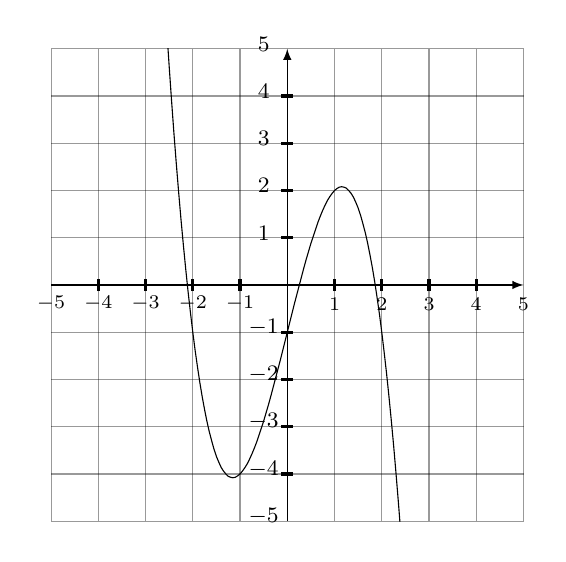
\begin{tikzpicture}[scale=.6]

    \tikzset{
      point/.style={
        thick,
        draw,
        cross out,
        inner sep=0pt,
        minimum width=5pt,
        minimum height=5pt,
      },
    }

    	
	\draw[color ={black},>=latex,->] (-5,0)--(5,0);
	\draw[color ={black},>=latex,->] (0,-5)--(0,5);
	\draw[color ={black},opacity = 0.4] (-5,1)--(5,1);
	\draw[color ={black},opacity = 0.4] (-5,2)--(5,2);
	\draw[color ={black},opacity = 0.4] (-5,3)--(5,3);
	\draw[color ={black},opacity = 0.4] (-5,4)--(5,4);
	\draw[color ={black},opacity = 0.4] (-5,5)--(5,5);
	\draw[color ={black},opacity = 0.4] (-5,-1)--(5,-1);
	\draw[color ={black},opacity = 0.4] (-5,-2)--(5,-2);
	\draw[color ={black},opacity = 0.4] (-5,-3)--(5,-3);
	\draw[color ={black},opacity = 0.4] (-5,-4)--(5,-4);
	\draw[color ={black},opacity = 0.4] (-5,-5)--(5,-5);
	\draw[color ={black},opacity = 0.4] (1,-5)--(1,5);
	\draw[color ={black},opacity = 0.4] (2,-5)--(2,5);
	\draw[color ={black},opacity = 0.4] (3,-5)--(3,5);
	\draw[color ={black},opacity = 0.4] (4,-5)--(4,5);
	\draw[color ={black},opacity = 0.4] (5,-5)--(5,5);
	\draw[color ={black},opacity = 0.4] (-1,-5)--(-1,5);
	\draw[color ={black},opacity = 0.4] (-2,-5)--(-2,5);
	\draw[color ={black},opacity = 0.4] (-3,-5)--(-3,5);
	\draw[color ={black},opacity = 0.4] (-4,-5)--(-4,5);
	\draw[color ={black},opacity = 0.4] (-5,-5)--(-5,5);
	\draw[color ={black},line width = 1.2] (1,-0.13)--(1,0.13);
	\draw[color ={black},line width = 1.2] (2,-0.13)--(2,0.13);
	\draw[color ={black},line width = 1.2] (3,-0.13)--(3,0.13);
	\draw[color ={black},line width = 1.2] (4,-0.13)--(4,0.13);
	\draw[color ={black},line width = 1.2] (-1,-0.13)--(-1,0.13);
	\draw[color ={black},line width = 1.2] (-2,-0.13)--(-2,0.13);
	\draw[color ={black},line width = 1.2] (-3,-0.13)--(-3,0.13);
	\draw[color ={black},line width = 1.2] (-4,-0.13)--(-4,0.13);
	\draw[color ={black},line width = 1.2] (-0.13,1)--(0.13,1);
	\draw[color ={black},line width = 1.2] (-0.13,2)--(0.13,2);
	\draw[color ={black},line width = 1.2] (-0.13,3)--(0.13,3);
	\draw[color ={black},line width = 1.2] (-0.13,4)--(0.13,4);
	\draw[color ={black},line width = 1.2] (-0.13,-1)--(0.13,-1);
	\draw[color ={black},line width = 1.2] (-0.13,-2)--(0.13,-2);
	\draw[color ={black},line width = 1.2] (-0.13,-3)--(0.13,-3);
	\draw[color ={black},line width = 1.2] (-0.13,-4)--(0.13,-4);
	\draw (1,-0.4) node[anchor = center] {\scriptsize \color{black}{$1$}};
	\draw (2,-0.4) node[anchor = center] {\scriptsize \color{black}{$2$}};
	\draw (3,-0.4) node[anchor = center] {\scriptsize \color{black}{$3$}};
	\draw (4,-0.4) node[anchor = center] {\scriptsize \color{black}{$4$}};
	\draw (5,-0.4) node[anchor = center] {\scriptsize \color{black}{$5$}};
	\draw (-1,-0.4) node[anchor = center] {\scriptsize \color{black}{$-1$}};
	\draw (-2,-0.4) node[anchor = center] {\scriptsize \color{black}{$-2$}};
	\draw (-3,-0.4) node[anchor = center] {\scriptsize \color{black}{$-3$}};
	\draw (-4,-0.4) node[anchor = center] {\scriptsize \color{black}{$-4$}};
	\draw (-5,-0.4) node[anchor = center] {\scriptsize \color{black}{$-5$}};
	\draw (-0.5,1.1) node[anchor = center] {\footnotesize \color{black}{$1$}};
	\draw (-0.5,2.1) node[anchor = center] {\footnotesize \color{black}{$2$}};
	\draw (-0.5,3.1) node[anchor = center] {\footnotesize \color{black}{$3$}};
	\draw (-0.5,4.1) node[anchor = center] {\footnotesize \color{black}{$4$}};
	\draw (-0.5,5.1) node[anchor = center] {\footnotesize \color{black}{$5$}};
	\draw (-0.5,-0.9) node[anchor = center] {\footnotesize \color{black}{$-1$}};
	\draw (-0.5,-1.9) node[anchor = center] {\footnotesize \color{black}{$-2$}};
	\draw (-0.5,-2.9) node[anchor = center] {\footnotesize \color{black}{$-3$}};
	\draw (-0.5,-3.9) node[anchor = center] {\footnotesize \color{black}{$-4$}};
	\draw (-0.5,-4.9) node[anchor = center] {\footnotesize \color{black}{$-5$}};
		    \clip (-5,-5) rectangle (5,5);
	\draw[color={black}] (-2.55,5.38)--(-2.5,4.63)--(-2.45,3.91)--(-2.4,3.22)--(-2.35,2.58)--(-2.3,1.97)--(-2.25,1.39)--(-2.2,0.85)--(-2.15,0.34)--(-2.1,-0.14)--(-2.05,-0.58)--(-2,-1)--(-1.95,-1.39)--(-1.9,-1.74)--(-1.85,-2.07)--(-1.8,-2.37)--(-1.75,-2.64)--(-1.7,-2.89)--(-1.65,-3.11)--(-1.6,-3.3)--(-1.55,-3.48)--(-1.5,-3.63)--(-1.45,-3.75)--(-1.4,-3.86)--(-1.35,-3.94)--(-1.3,-4)--(-1.25,-4.05)--(-1.2,-4.07)--(-1.15,-4.08)--(-1.1,-4.07)--(-1.05,-4.04)--(-1,-4)--(-0.95,-3.94)--(-0.9,-3.87)--(-0.85,-3.79)--(-0.8,-3.69)--(-0.75,-3.58)--(-0.7,-3.46)--(-0.65,-3.33)--(-0.6,-3.18)--(-0.55,-3.03)--(-0.5,-2.88)--(-0.45,-2.71)--(-0.4,-2.54)--(-0.35,-2.36)--(-0.3,-2.17)--(-0.25,-1.98)--(-0.2,-1.79)--(-0.15,-1.6)--(-0.1,-1.4)--(-0.05,-1.2)--(0,-1)--(0.05,-0.8)--(0.1,-0.6)--(0.15,-0.4)--(0.2,-0.21)--(0.25,-0.02)--(0.3,0.17)--(0.35,0.36)--(0.4,0.54)--(0.45,0.71)--(0.5,0.88)--(0.55,1.03)--(0.6,1.18)--(0.65,1.33)--(0.7,1.46)--(0.75,1.58)--(0.8,1.69)--(0.85,1.79)--(0.9,1.87)--(0.95,1.94)--(1,2)--(1.05,2.04)--(1.1,2.07)--(1.15,2.08)--(1.2,2.07)--(1.25,2.05)--(1.3,2)--(1.35,1.94)--(1.4,1.86)--(1.45,1.75)--(1.5,1.63)--(1.55,1.48)--(1.6,1.3)--(1.65,1.11)--(1.7,0.89)--(1.75,0.64)--(1.8,0.37)--(1.85,0.07)--(1.9,-0.26)--(1.95,-0.61)--(2,-1)--(2.05,-1.42)--(2.1,-1.86)--(2.15,-2.34)--(2.2,-2.85)--(2.25,-3.39)--(2.3,-3.97)--(2.35,-4.58)--(2.4,-5.22)--(2.45,-5.91);

\end{tikzpicture}\\Quel est l'ensemble de définition de la fonction représentée ci-dessus ?
\end{Exercice}

% @see : https://coopmaths.fr/alea?uuid=e46e6&id=200F3-02&n=1&d=10&s=1&alea=pThR&cd=1&cols=1
\begin{Exercice}%4

\begin{tikzpicture}[scale=.6]

    \tikzset{
      point/.style={
        thick,
        draw,
        cross out,
        inner sep=0pt,
        minimum width=5pt,
        minimum height=5pt,
      },
    }
    \clip (-7.5,-5.5) rectangle (8.5,5.5);
    	
	\draw[color ={black},>=latex,->] (-6,0)--(7,0);
	\draw[color ={black},>=latex,->] (0,-4)--(0,4);
	\draw[color ={black},opacity = 0.4] (-6,1)--(7,1);
	\draw[color ={black},opacity = 0.4] (-6,2)--(7,2);
	\draw[color ={black},opacity = 0.4] (-6,3)--(7,3);
	\draw[color ={black},opacity = 0.4] (-6,4)--(7,4);
	\draw[color ={black},opacity = 0.4] (-6,-1)--(7,-1);
	\draw[color ={black},opacity = 0.4] (-6,-2)--(7,-2);
	\draw[color ={black},opacity = 0.4] (-6,-3)--(7,-3);
	\draw[color ={black},opacity = 0.4] (-6,-4)--(7,-4);
	\draw[color ={black},opacity = 0.4] (1,-4)--(1,4);
	\draw[color ={black},opacity = 0.4] (2,-4)--(2,4);
	\draw[color ={black},opacity = 0.4] (3,-4)--(3,4);
	\draw[color ={black},opacity = 0.4] (4,-4)--(4,4);
	\draw[color ={black},opacity = 0.4] (5,-4)--(5,4);
	\draw[color ={black},opacity = 0.4] (6,-4)--(6,4);
	\draw[color ={black},opacity = 0.4] (7,-4)--(7,4);
	\draw[color ={black},opacity = 0.4] (-1,-4)--(-1,4);
	\draw[color ={black},opacity = 0.4] (-2,-4)--(-2,4);
	\draw[color ={black},opacity = 0.4] (-3,-4)--(-3,4);
	\draw[color ={black},opacity = 0.4] (-4,-4)--(-4,4);
	\draw[color ={black},opacity = 0.4] (-5,-4)--(-5,4);
	\draw[color ={black},opacity = 0.4] (-6,-4)--(-6,4);
	\draw[color ={black},line width = 1.2] (1,-0.13)--(1,0.13);
	\draw[color ={black},line width = 1.2] (2,-0.13)--(2,0.13);
	\draw[color ={black},line width = 1.2] (3,-0.13)--(3,0.13);
	\draw[color ={black},line width = 1.2] (4,-0.13)--(4,0.13);
	\draw[color ={black},line width = 1.2] (5,-0.13)--(5,0.13);
	\draw[color ={black},line width = 1.2] (6,-0.13)--(6,0.13);
	\draw[color ={black},line width = 1.2] (-1,-0.13)--(-1,0.13);
	\draw[color ={black},line width = 1.2] (-2,-0.13)--(-2,0.13);
	\draw[color ={black},line width = 1.2] (-3,-0.13)--(-3,0.13);
	\draw[color ={black},line width = 1.2] (-4,-0.13)--(-4,0.13);
	\draw[color ={black},line width = 1.2] (-5,-0.13)--(-5,0.13);
	\draw[color ={black},line width = 1.2] (-0.13,1)--(0.13,1);
	\draw[color ={black},line width = 1.2] (-0.13,2)--(0.13,2);
	\draw[color ={black},line width = 1.2] (-0.13,3)--(0.13,3);
	\draw[color ={black},line width = 1.2] (-0.13,-1)--(0.13,-1);
	\draw[color ={black},line width = 1.2] (-0.13,-2)--(0.13,-2);
	\draw[color ={black},line width = 1.2] (-0.13,-3)--(0.13,-3);
	\draw (1,-0.4) node[anchor = center] {\scriptsize \color{black}{$1$}};
	\draw (2,-0.4) node[anchor = center] {\scriptsize \color{black}{$2$}};
	\draw (3,-0.4) node[anchor = center] {\scriptsize \color{black}{$3$}};
	\draw (4,-0.4) node[anchor = center] {\scriptsize \color{black}{$4$}};
	\draw (5,-0.4) node[anchor = center] {\scriptsize \color{black}{$5$}};
	\draw (6,-0.4) node[anchor = center] {\scriptsize \color{black}{$6$}};
	\draw (7,-0.4) node[anchor = center] {\scriptsize \color{black}{$7$}};
	\draw (-1,-0.4) node[anchor = center] {\scriptsize \color{black}{$-1$}};
	\draw (-2,-0.4) node[anchor = center] {\scriptsize \color{black}{$-2$}};
	\draw (-3,-0.4) node[anchor = center] {\scriptsize \color{black}{$-3$}};
	\draw (-4,-0.4) node[anchor = center] {\scriptsize \color{black}{$-4$}};
	\draw (-5,-0.4) node[anchor = center] {\scriptsize \color{black}{$-5$}};
	\draw (-6,-0.4) node[anchor = center] {\scriptsize \color{black}{$-6$}};
	\draw (-0.5,1.1) node[anchor = center] {\footnotesize \color{black}{$1$}};
	\draw (-0.5,2.1) node[anchor = center] {\footnotesize \color{black}{$2$}};
	\draw (-0.5,3.1) node[anchor = center] {\footnotesize \color{black}{$3$}};
	\draw (-0.5,4.1) node[anchor = center] {\footnotesize \color{black}{$4$}};
	\draw (-0.5,-0.9) node[anchor = center] {\footnotesize \color{black}{$-1$}};
	\draw (-0.5,-1.9) node[anchor = center] {\footnotesize \color{black}{$-2$}};
	\draw (-0.5,-2.9) node[anchor = center] {\footnotesize \color{black}{$-3$}};
	\draw (-0.5,-3.9) node[anchor = center] {\footnotesize \color{black}{$-4$}};
	
	\draw[color = {Couleur10},line width = 1, opacity = 1](-4,1) .. controls +(1.00,1.00) and +(-1.00,0.00)  .. (-1.00,2.00)
 .. controls +(1.00,0.00) and +(-1.00,0.00)  .. (2.00,-2.00)
 .. controls +(1.00,0.00) and +(-1.00,-1.00)  .. (5.00,1.00)
;

	
	 \filldraw[color={Couleur10},fill={black}] (-4,1) circle (0.05);
	
	 \filldraw[color={Couleur10},fill={black}] (5,1) circle (0.05);

\end{tikzpicture}\\Quel est l'ensemble de définition de la fonction représentée ci-dessus ?
\end{Exercice}

\end{multicols}

\newpage

% @see : https://coopmaths.fr/alea?uuid=36795&id=2F20-1&n=2&d=10&s=1&s2=1&alea=7bbw&cd=0&cols=1
\begin{Exercice}%5
\leavevmode\vspace{-\baselineskip}
\begin{enumerate}[itemsep=1em]
	\item \begin{minipage}[t]{\linewidth}Soit $f$ la fonction définie sur $\mathbb{R}$ par :
              \begin{center}
$f(x)=-4x-1$
\end{center}
              On note $\mathscr{C}_f$ la courbe représentative de la fonction $f$ dans un repère.\\
              Le point $A(4; -21)$ appartient-il à $\mathscr{C}_f$ ? Justifier.\end{minipage}
	\item \begin{minipage}[t]{\linewidth}Soit $f$ la fonction définie sur $\mathbb{R}$ par :
              \begin{center}
$f(x)=5x-9$
\end{center}
              On note $\mathscr{C}_f$ la courbe représentative de la fonction $f$ dans un repère.\\
              Le point $A(-7; -39)$ appartient-il à $\mathscr{C}_f$ ? Justifier.\end{minipage}
\end{enumerate}
\vspace{-0.5cm}
\end{Exercice}



% @see : https://coopmaths.fr/alea?uuid=ec059&id=2F20-2&n=2&d=10&s=1&s2=1&alea=vsqC&cd=1&cols=1
\begin{Exercice}%6
\leavevmode\vspace{-\baselineskip}
\begin{enumerate}[itemsep=1em]
	\item \begin{minipage}[t]{\linewidth}Soit $w$ la fonction définie sur $\mathbb{R}$ par :
              \begin{center}
$w(x)=-x-11$
\end{center}
              On note $\mathscr{C}$ la courbe représentative de la fonction $w$ dans un repère.\\
             $R$ est le point de $\mathscr{C}$ d'abscisse $6$. \\Quelle est son ordonnée ? \end{minipage}
	\item \begin{minipage}[t]{\linewidth}Soit $v$ la fonction définie sur $\mathbb{R}$ par :
              \begin{center}
$v(x)=3x+4$
\end{center}
              On note $\mathscr{C}$ la courbe représentative de la fonction $v$ dans un repère.\\
             $N$ est le point de $\mathscr{C}$ d'abscisse $-7$. \\Quelle est son ordonnée ? \end{minipage}
\end{enumerate}
\vspace{-0.5cm}
\end{Exercice}

\begin{multicols}{2}
% @see : https://coopmaths.fr/alea?uuid=a2ac2&id=2F22-1&n=1&d=10&alea=ajcv&cd=1&cols=1
\begin{Exercice}%7

Voici la représentation graphique $\mathscr{C}_f$ d'une fonction $f$ définie sur $[-3\,;\,8]$.\\\begin{tikzpicture}[baseline,scale = 0.6]

    \tikzset{
      point/.style={
        thick,
        draw,
        cross out,
        inner sep=0pt,
        minimum width=5pt,
        minimum height=5pt,
      },
    }
    \clip (-5.5,-5.5) rectangle (10.5,5.5);
    	
	\draw[color ={black},line width = 1.5,>=latex,->] (-4,0)--(9,0);
	\draw[color ={black},line width = 1.5,>=latex,->] (0,-4)--(0,4);
	\draw[color ={gray},opacity = 0.3] (-4,0)--(9,0);
	\draw[color ={gray},opacity = 0.3] (-4,1)--(9,1);
	\draw[color ={gray},opacity = 0.3] (-4,2)--(9,2);
	\draw[color ={gray},opacity = 0.3] (-4,3)--(9,3);
	\draw[color ={gray},opacity = 0.3] (-4,4)--(9,4);
	\draw[color ={gray},opacity = 0.3] (-4,0)--(9,0);
	\draw[color ={gray},opacity = 0.3] (-4,-1)--(9,-1);
	\draw[color ={gray},opacity = 0.3] (-4,-2)--(9,-2);
	\draw[color ={gray},opacity = 0.3] (-4,-3)--(9,-3);
	\draw[color ={gray},opacity = 0.3] (-4,-4)--(9,-4);
	\draw[color ={gray},opacity = 0.3] (0,-4)--(0,4);
	\draw[color ={gray},opacity = 0.3] (1,-4)--(1,4);
	\draw[color ={gray},opacity = 0.3] (2,-4)--(2,4);
	\draw[color ={gray},opacity = 0.3] (3,-4)--(3,4);
	\draw[color ={gray},opacity = 0.3] (4,-4)--(4,4);
	\draw[color ={gray},opacity = 0.3] (5,-4)--(5,4);
	\draw[color ={gray},opacity = 0.3] (6,-4)--(6,4);
	\draw[color ={gray},opacity = 0.3] (7,-4)--(7,4);
	\draw[color ={gray},opacity = 0.3] (8,-4)--(8,4);
	\draw[color ={gray},opacity = 0.3] (9,-4)--(9,4);
	\draw[color ={gray},opacity = 0.3] (0,-4)--(0,4);
	\draw[color ={gray},opacity = 0.3] (-1,-4)--(-1,4);
	\draw[color ={gray},opacity = 0.3] (-2,-4)--(-2,4);
	\draw[color ={gray},opacity = 0.3] (-3,-4)--(-3,4);
	\draw[color ={gray},opacity = 0.3] (-4,-4)--(-4,4);
	\draw[color ={black},line width = 1.2] (1,-0.1)--(1,0.1);
	\draw[color ={black},line width = 1.2] (2,-0.1)--(2,0.1);
	\draw[color ={black},line width = 1.2] (3,-0.1)--(3,0.1);
	\draw[color ={black},line width = 1.2] (4,-0.1)--(4,0.1);
	\draw[color ={black},line width = 1.2] (5,-0.1)--(5,0.1);
	\draw[color ={black},line width = 1.2] (6,-0.1)--(6,0.1);
	\draw[color ={black},line width = 1.2] (7,-0.1)--(7,0.1);
	\draw[color ={black},line width = 1.2] (8,-0.1)--(8,0.1);
	\draw[color ={black},line width = 1.2] (-1,-0.1)--(-1,0.1);
	\draw[color ={black},line width = 1.2] (-2,-0.1)--(-2,0.1);
	\draw[color ={black},line width = 1.2] (-3,-0.1)--(-3,0.1);
	\draw[color ={black},line width = 1.2] (-0.1,1)--(0.1,1);
	\draw[color ={black},line width = 1.2] (-0.1,2)--(0.1,2);
	\draw[color ={black},line width = 1.2] (-0.1,3)--(0.1,3);
	\draw[color ={black},line width = 1.2] (-0.1,-1)--(0.1,-1);
	\draw[color ={black},line width = 1.2] (-0.1,-2)--(0.1,-2);
	\draw[color ={black},line width = 1.2] (-0.1,-3)--(0.1,-3);
	\draw (1,-0.4) node[anchor = center] {\scriptsize \color{black}{$1$}};
	\draw (2,-0.4) node[anchor = center] {\scriptsize \color{black}{$2$}};
	\draw (3,-0.4) node[anchor = center] {\scriptsize \color{black}{$3$}};
	\draw (4,-0.4) node[anchor = center] {\scriptsize \color{black}{$4$}};
	\draw (5,-0.4) node[anchor = center] {\scriptsize \color{black}{$5$}};
	\draw (6,-0.4) node[anchor = center] {\scriptsize \color{black}{$6$}};
	\draw (7,-0.4) node[anchor = center] {\scriptsize \color{black}{$7$}};
	\draw (8,-0.4) node[anchor = center] {\scriptsize \color{black}{$8$}};
	\draw (-1,-0.4) node[anchor = center] {\scriptsize \color{black}{$-1$}};
	\draw (-2,-0.4) node[anchor = center] {\scriptsize \color{black}{$-2$}};
	\draw (-3,-0.4) node[anchor = center] {\scriptsize \color{black}{$-3$}};
	\draw (-0.6,1.1) node[anchor = center] {\footnotesize \color{black}{$1$}};
	\draw (-0.6,2.1) node[anchor = center] {\footnotesize \color{black}{$2$}};
	\draw (-0.6,3.1) node[anchor = center] {\footnotesize \color{black}{$3$}};
	\draw (-0.6,-0.9) node[anchor = center] {\footnotesize \color{black}{$-1$}};
	\draw (-0.6,-1.9) node[anchor = center] {\footnotesize \color{black}{$-2$}};
	\draw (-0.6,-2.9) node[anchor = center] {\footnotesize \color{black}{$-3$}};
	
	\draw[color = {Couleur10},line width = 1.2, opacity = 1](-3,0) .. controls +(0.33,0.00) and +(-0.33,-0.50)  .. (-2.00,2.00)
 .. controls +(0.33,0.50) and +(-0.33,0.00)  .. (-1.00,3.00)
 .. controls +(0.33,0.00) and +(-0.33,0.50)  .. (0.00,2.00)
 .. controls +(0.33,-0.50) and +(-0.33,0.83)  .. (1.00,-1.00)
 .. controls +(0.33,-0.83) and +(-0.33,0.00)  .. (2.00,-3.00)
 .. controls +(0.33,0.00) and +(-0.33,-0.67)  .. (3.00,-1.00)
 .. controls +(0.33,0.67) and +(-0.33,-0.67)  .. (4.00,2.00)
 .. controls +(0.33,0.67) and +(-0.33,0.00)  .. (5.00,3.00)
 .. controls +(0.33,0.00) and +(-0.33,0.67)  .. (6.00,2.00)
 .. controls +(0.33,-0.67) and +(-0.33,0.67)  .. (7.00,-1.00)
 .. controls +(0.33,-0.67) and +(-0.33,0.17)  .. (8.00,-2.00)
;

	 \filldraw[color={Couleur10},fill={{Couleur10}}] (-3,0) circle (0.07500000000000001);
	 \filldraw[color={Couleur10},fill={{Couleur10}}] (-2,2) circle (0.07500000000000001);
	 \filldraw[color={Couleur10},fill={{Couleur10}}] (-1,3) circle (0.07500000000000001);
	 \filldraw[color={Couleur10},fill={{Couleur10}}] (0,2) circle (0.07500000000000001);
	 \filldraw[color={Couleur10},fill={{Couleur10}}] (1,-1) circle (0.07500000000000001);
	 \filldraw[color={Couleur10},fill={{Couleur10}}] (2,-3) circle (0.07500000000000001);
	 \filldraw[color={Couleur10},fill={{Couleur10}}] (3,-1) circle (0.07500000000000001);
	 \filldraw[color={Couleur10},fill={{Couleur10}}] (4,2) circle (0.07500000000000001);
	 \filldraw[color={Couleur10},fill={{Couleur10}}] (5,3) circle (0.07500000000000001);
	 \filldraw[color={Couleur10},fill={{Couleur10}}] (6,2) circle (0.07500000000000001);
	 \filldraw[color={Couleur10},fill={{Couleur10}}] (7,-1) circle (0.07500000000000001);
	 \filldraw[color={Couleur10},fill={{Couleur10}}] (8,-2) circle (0.07500000000000001);
	\draw [color={black}] (-0.3,-0.3) node[anchor = center,scale=1, rotate = 0] {O};

\end{tikzpicture}\\Répondre aux questions en utilisant le graphique.\\\textbf {a.} Quel est le nombre de solutions de l'équation $f(x)=-3$ ?\\\textbf {b.} Résoudre l'équation $f(x)=4$.\\\textbf {c.} Déterminer une valeur de $k$ telle que $f(x)=k$ admette exactement $3$ solutions.

\end{Exercice}

\columnbreak

% @see : https://coopmaths.fr/alea?uuid=a2ac2&id=2F22-1&n=1&d=10&alea=9fxO&cd=1&cols=1
\begin{Exercice}%8

Voici la représentation graphique $\mathscr{C}_f$ d'une fonction $f$ définie sur $[-6\,;\,5]$.\\\begin{tikzpicture}[baseline,scale = 0.6]

    \tikzset{
      point/.style={
        thick,
        draw,
        cross out,
        inner sep=0pt,
        minimum width=5pt,
        minimum height=5pt,
      },
    }
    \clip (-8.5,-6.5) rectangle (7.5,4.5);
    	
	\draw[color ={black},line width = 1.5,>=latex,->] (-7,0)--(6,0);
	\draw[color ={black},line width = 1.5,>=latex,->] (0,-5)--(0,3);
	\draw[color ={gray},opacity = 0.3] (-7,0)--(6,0);
	\draw[color ={gray},opacity = 0.3] (-7,1)--(6,1);
	\draw[color ={gray},opacity = 0.3] (-7,2)--(6,2);
	\draw[color ={gray},opacity = 0.3] (-7,3)--(6,3);
	\draw[color ={gray},opacity = 0.3] (-7,0)--(6,0);
	\draw[color ={gray},opacity = 0.3] (-7,-1)--(6,-1);
	\draw[color ={gray},opacity = 0.3] (-7,-2)--(6,-2);
	\draw[color ={gray},opacity = 0.3] (-7,-3)--(6,-3);
	\draw[color ={gray},opacity = 0.3] (-7,-4)--(6,-4);
	\draw[color ={gray},opacity = 0.3] (-7,-5)--(6,-5);
	\draw[color ={gray},opacity = 0.3] (0,-5)--(0,3);
	\draw[color ={gray},opacity = 0.3] (1,-5)--(1,3);
	\draw[color ={gray},opacity = 0.3] (2,-5)--(2,3);
	\draw[color ={gray},opacity = 0.3] (3,-5)--(3,3);
	\draw[color ={gray},opacity = 0.3] (4,-5)--(4,3);
	\draw[color ={gray},opacity = 0.3] (5,-5)--(5,3);
	\draw[color ={gray},opacity = 0.3] (6,-5)--(6,3);
	\draw[color ={gray},opacity = 0.3] (0,-5)--(0,3);
	\draw[color ={gray},opacity = 0.3] (-1,-5)--(-1,3);
	\draw[color ={gray},opacity = 0.3] (-2,-5)--(-2,3);
	\draw[color ={gray},opacity = 0.3] (-3,-5)--(-3,3);
	\draw[color ={gray},opacity = 0.3] (-4,-5)--(-4,3);
	\draw[color ={gray},opacity = 0.3] (-5,-5)--(-5,3);
	\draw[color ={gray},opacity = 0.3] (-6,-5)--(-6,3);
	\draw[color ={gray},opacity = 0.3] (-7,-5)--(-7,3);
	\draw[color ={black},line width = 1.2] (1,-0.1)--(1,0.1);
	\draw[color ={black},line width = 1.2] (2,-0.1)--(2,0.1);
	\draw[color ={black},line width = 1.2] (3,-0.1)--(3,0.1);
	\draw[color ={black},line width = 1.2] (4,-0.1)--(4,0.1);
	\draw[color ={black},line width = 1.2] (5,-0.1)--(5,0.1);
	\draw[color ={black},line width = 1.2] (-1,-0.1)--(-1,0.1);
	\draw[color ={black},line width = 1.2] (-2,-0.1)--(-2,0.1);
	\draw[color ={black},line width = 1.2] (-3,-0.1)--(-3,0.1);
	\draw[color ={black},line width = 1.2] (-4,-0.1)--(-4,0.1);
	\draw[color ={black},line width = 1.2] (-5,-0.1)--(-5,0.1);
	\draw[color ={black},line width = 1.2] (-6,-0.1)--(-6,0.1);
	\draw[color ={black},line width = 1.2] (-0.1,1)--(0.1,1);
	\draw[color ={black},line width = 1.2] (-0.1,2)--(0.1,2);
	\draw[color ={black},line width = 1.2] (-0.1,-1)--(0.1,-1);
	\draw[color ={black},line width = 1.2] (-0.1,-2)--(0.1,-2);
	\draw[color ={black},line width = 1.2] (-0.1,-3)--(0.1,-3);
	\draw[color ={black},line width = 1.2] (-0.1,-4)--(0.1,-4);
	\draw (1,-0.4) node[anchor = center] {\scriptsize \color{black}{$1$}};
	\draw (2,-0.4) node[anchor = center] {\scriptsize \color{black}{$2$}};
	\draw (3,-0.4) node[anchor = center] {\scriptsize \color{black}{$3$}};
	\draw (4,-0.4) node[anchor = center] {\scriptsize \color{black}{$4$}};
	\draw (5,-0.4) node[anchor = center] {\scriptsize \color{black}{$5$}};
	\draw (-1,-0.4) node[anchor = center] {\scriptsize \color{black}{$-1$}};
	\draw (-2,-0.4) node[anchor = center] {\scriptsize \color{black}{$-2$}};
	\draw (-3,-0.4) node[anchor = center] {\scriptsize \color{black}{$-3$}};
	\draw (-4,-0.4) node[anchor = center] {\scriptsize \color{black}{$-4$}};
	\draw (-5,-0.4) node[anchor = center] {\scriptsize \color{black}{$-5$}};
	\draw (-6,-0.4) node[anchor = center] {\scriptsize \color{black}{$-6$}};
	\draw (-0.6,1.1) node[anchor = center] {\footnotesize \color{black}{$1$}};
	\draw (-0.6,2.1) node[anchor = center] {\footnotesize \color{black}{$2$}};
	\draw (-0.6,-0.9) node[anchor = center] {\footnotesize \color{black}{$-1$}};
	\draw (-0.6,-1.9) node[anchor = center] {\footnotesize \color{black}{$-2$}};
	\draw (-0.6,-2.9) node[anchor = center] {\footnotesize \color{black}{$-3$}};
	\draw (-0.6,-3.9) node[anchor = center] {\footnotesize \color{black}{$-4$}};
	
	\draw[color = {Couleur10},line width = 1.2, opacity = 1](-6,-4) .. controls +(0.33,0.07) and +(-0.33,-0.33)  .. (-5.00,-3.00)
 .. controls +(0.33,0.33) and +(-0.33,0.00)  .. (-4.00,-2.00)
 .. controls +(0.33,0.00) and +(-0.33,0.67)  .. (-3.00,-3.00)
 .. controls +(0.33,-0.67) and +(-0.33,0.00)  .. (-2.00,-4.00)
 .. controls +(0.33,0.00) and +(-0.33,-1.00)  .. (-1.00,-2.00)
 .. controls +(0.33,1.00) and +(-0.33,-0.33)  .. (0.00,1.00)
 .. controls +(0.33,0.33) and +(-0.33,0.00)  .. (1.00,2.00)
 .. controls +(0.33,0.00) and +(-0.33,0.50)  .. (2.00,1.00)
 .. controls +(0.33,-0.33) and +(-0.33,0.67)  .. (3.00,0.00)
 .. controls +(0.33,-0.67) and +(-0.33,0.00)  .. (4.00,-2.00)
 .. controls +(0.33,0.00) and +(-0.33,-0.50)  .. (5.00,0.00)
;

	 \filldraw[color={Couleur10},fill={{Couleur10}}] (-6,-4) circle (0.07500000000000001);
	 \filldraw[color={Couleur10},fill={{Couleur10}}] (5,0) circle (0.07500000000000001);
	\draw [color={black}] (-0.3,-0.3) node[anchor = center,scale=1, rotate = 0] {O};

\end{tikzpicture}\\Répondre aux questions en utilisant le graphique.\\\textbf {a.} Quel est le nombre de solutions de l'équation $f(x)=-2$ ?\\\textbf {b.} Résoudre l'équation $f(x)=3$.\\\textbf {c.} Déterminer une valeur de $k$ telle que $f(x)=k$ admette exactement $1$ solution.
\end{Exercice}
\end{multicols}

\newpage

\begin{multicols}{2}
% @see : https://coopmaths.fr/alea?uuid=28997&id=2F20-4&n=1&d=10&s=1&s2=10&s3=false&alea=QYkR&cd=1&cols=1
\begin{Exercice}%9

On considère les fonctions $m$ et $d$ définies sur $\R$ et dont on a représenté ci-dessous leurs courbes respectives.

\medskip
Résoudre graphiquement l'équation $m(x){\color{black}\boldsymbol{~=~}}d(x)$ sur la partie visible du graphique.\\\begin{tikzpicture}[scale=.5]

    \tikzset{
      point/.style={
        thick,
        draw,
        cross out,
        inner sep=0pt,
        minimum width=5pt,
        minimum height=5pt,
      },
    }

    	\draw[color ={black},>=latex,->] (-7.2,0)--(3.2,0);
	\draw[color ={black},>=latex,->] (0,-5.5)--(0,6.9);
	\draw[color ={black},opacity = 0.4] (-7.2,1)--(3.2,1);
	\draw[color ={black},opacity = 0.4] (-7.2,2)--(3.2,2);
	\draw[color ={black},opacity = 0.4] (-7.2,3)--(3.2,3);
	\draw[color ={black},opacity = 0.4] (-7.2,4)--(3.2,4);
	\draw[color ={black},opacity = 0.4] (-7.2,5)--(3.2,5);
	\draw[color ={black},opacity = 0.4] (-7.2,6)--(3.2,6);
	\draw[color ={black},opacity = 0.4] (-7.2,-1)--(3.2,-1);
	\draw[color ={black},opacity = 0.4] (-7.2,-2)--(3.2,-2);
	\draw[color ={black},opacity = 0.4] (-7.2,-3)--(3.2,-3);
	\draw[color ={black},opacity = 0.4] (-7.2,-4)--(3.2,-4);
	\draw[color ={black},opacity = 0.4] (-7.2,-5)--(3.2,-5);
	\draw[color ={black},opacity = 0.4] (1,-5.5)--(1,6.9);
	\draw[color ={black},opacity = 0.4] (2,-5.5)--(2,6.9);
	\draw[color ={black},opacity = 0.4] (3,-5.5)--(3,6.9);
	\draw[color ={black},opacity = 0.4] (-1,-5.5)--(-1,6.9);
	\draw[color ={black},opacity = 0.4] (-2,-5.5)--(-2,6.9);
	\draw[color ={black},opacity = 0.4] (-3,-5.5)--(-3,6.9);
	\draw[color ={black},opacity = 0.4] (-4,-5.5)--(-4,6.9);
	\draw[color ={black},opacity = 0.4] (-5,-5.5)--(-5,6.9);
	\draw[color ={black},opacity = 0.4] (-6,-5.5)--(-6,6.9);
	\draw[color ={black},opacity = 0.4] (-7,-5.5)--(-7,6.9);

	
	\draw[color ={black},line width = 1.2] (1,-0.13)--(1,0.13);
	\draw[color ={black},line width = 1.2] (2,-0.13)--(2,0.13);
	\draw[color ={black},line width = 1.2] (-1,-0.13)--(-1,0.13);
	\draw[color ={black},line width = 1.2] (-2,-0.13)--(-2,0.13);
	\draw[color ={black},line width = 1.2] (-3,-0.13)--(-3,0.13);
	\draw[color ={black},line width = 1.2] (-4,-0.13)--(-4,0.13);
	\draw[color ={black},line width = 1.2] (-5,-0.13)--(-5,0.13);
	\draw[color ={black},line width = 1.2] (-6,-0.13)--(-6,0.13);
	\draw[color ={black},line width = 1.2] (-0.13,1)--(0.13,1);
	\draw[color ={black},line width = 1.2] (-0.13,2)--(0.13,2);
	\draw[color ={black},line width = 1.2] (-0.13,3)--(0.13,3);
	\draw[color ={black},line width = 1.2] (-0.13,4)--(0.13,4);
	\draw[color ={black},line width = 1.2] (-0.13,5)--(0.13,5);
	\draw[color ={black},line width = 1.2] (-0.13,-1)--(0.13,-1);
	\draw[color ={black},line width = 1.2] (-0.13,-2)--(0.13,-2);
	\draw[color ={black},line width = 1.2] (-0.13,-3)--(0.13,-3);
	\draw[color ={black},line width = 1.2] (-0.13,-4)--(0.13,-4);
	\draw (1,-0.4) node[anchor = center] {\scriptsize \color{black}{$1$}};
	\draw (2,-0.4) node[anchor = center] {\scriptsize \color{black}{$2$}};
	\draw (3,-0.4) node[anchor = center] {\scriptsize \color{black}{$3$}};
	\draw (-1,-0.4) node[anchor = center] {\scriptsize \color{black}{$-1$}};
	\draw (-2,-0.4) node[anchor = center] {\scriptsize \color{black}{$-2$}};
	\draw (-3,-0.4) node[anchor = center] {\scriptsize \color{black}{$-3$}};
	\draw (-4,-0.4) node[anchor = center] {\scriptsize \color{black}{$-4$}};
	\draw (-5,-0.4) node[anchor = center] {\scriptsize \color{black}{$-5$}};
	\draw (-6,-0.4) node[anchor = center] {\scriptsize \color{black}{$-6$}};
	\draw (-7,-0.4) node[anchor = center] {\scriptsize \color{black}{$-7$}};
	\draw (-0.5,1.1) node[anchor = center] {\footnotesize \color{black}{$1$}};
	\draw (-0.5,2.1) node[anchor = center] {\footnotesize \color{black}{$2$}};
	\draw (-0.5,3.1) node[anchor = center] {\footnotesize \color{black}{$3$}};
	\draw (-0.5,4.1) node[anchor = center] {\footnotesize \color{black}{$4$}};
	\draw (-0.5,5.1) node[anchor = center] {\footnotesize \color{black}{$5$}};
	\draw (-0.5,6.1) node[anchor = center] {\footnotesize \color{black}{$6$}};
	\draw (-0.5,-0.9) node[anchor = center] {\footnotesize \color{black}{$-1$}};
	\draw (-0.5,-1.9) node[anchor = center] {\footnotesize \color{black}{$-2$}};
	\draw (-0.5,-2.9) node[anchor = center] {\footnotesize \color{black}{$-3$}};
	\draw (-0.5,-3.9) node[anchor = center] {\footnotesize \color{black}{$-4$}};
	\draw (-0.5,-4.9) node[anchor = center] {\footnotesize \color{black}{$-5$}};
	\draw[color ={Couleur10},line width = 1] (-7,2)--(3,2);
	    \clip (-7,-5) rectangle (3,6);
	\draw[color={Couleur6},line width = 1] (-7,-5)--(-6.8,-3.2)--(-6.6,-1.61)--(-6.4,-0.22)--(-6.2,0.98)--(-6,2)--(-5.8,2.85)--(-5.6,3.54)--(-5.4,4.07)--(-5.2,4.46)--(-5,4.72)--(-4.8,4.86)--(-4.6,4.87)--(-4.4,4.79)--(-4.2,4.6)--(-4,4.33)--(-3.8,3.98)--(-3.6,3.57)--(-3.4,3.09)--(-3.2,2.57)--(-3,2)--(-2.8,1.4)--(-2.6,0.78)--(-2.4,0.15)--(-2.2,-0.48)--(-2,-1.11)--(-1.8,-1.72)--(-1.6,-2.31)--(-1.4,-2.87)--(-1.2,-3.38)--(-1,-3.83)--(-0.8,-4.23)--(-0.6,-4.55)--(-0.4,-4.79)--(-0.2,-4.95)--(0,-5)--(0.2,-4.94)--(0.4,-4.77)--(0.6,-4.47)--(0.8,-4.03)--(1,-3.44)--(1.2,-2.7)--(1.4,-1.8)--(1.6,-0.72)--(1.8,0.54)--(2,2)--(2.2,3.66)--(2.4,5.53)--(2.6,7.62);
	\draw[color ={Couleur10},line width = 1] (-6,5.7)--(-5,5.7);
	\draw[color ={Couleur6},line width = 1] (-6,4.7)--(-5,4.7);
	\draw (-6.5,5.7) node[anchor = center] {\normalsize \color{Couleur10}{$\mathscr{C}_m$}};
	\draw (-6.5,4.7) node[anchor = center] {\normalsize \color{Couleur6}{$\mathscr{C}_d$}};

\end{tikzpicture}\\

\end{Exercice}

% @see : https://coopmaths.fr/alea?uuid=28997&id=2F20-4&n=1&d=10&s=1&s2=10&s3=false&alea=ajcv&cd=1&cols=1
\begin{Exercice}%10

On considère les fonctions $c$ et $k$ définies sur $\R$ et dont on a représenté ci-dessous leurs courbes respectives.

\medskip
Résoudre graphiquement l'équation $c(x){\color{black}\boldsymbol{~=~}}k(x)$ sur la partie visible du graphique.\\\begin{tikzpicture}[scale=.5]

    \tikzset{
      point/.style={
        thick,
        draw,
        cross out,
        inner sep=0pt,
        minimum width=5pt,
        minimum height=5pt,
      },
    }
    \clip (-5,-3.5) rectangle (6.7,10.399999999999999);
    	\draw[color ={black},>=latex,->] (-5.2,0)--(5.2,0);
	\draw[color ={black},>=latex,->] (0,-3.5)--(0,8.899999999999999);
	\draw[color ={black},opacity = 0.4] (-5.2,1)--(5.2,1);
	\draw[color ={black},opacity = 0.4] (-5.2,2)--(5.2,2);
	\draw[color ={black},opacity = 0.4] (-5.2,3)--(5.2,3);
	\draw[color ={black},opacity = 0.4] (-5.2,4)--(5.2,4);
	\draw[color ={black},opacity = 0.4] (-5.2,5)--(5.2,5);
	\draw[color ={black},opacity = 0.4] (-5.2,6)--(5.2,6);
	\draw[color ={black},opacity = 0.4] (-5.2,7)--(5.2,7);
	\draw[color ={black},opacity = 0.4] (-5.2,8)--(5.2,8);
	\draw[color ={black},opacity = 0.4] (-5.2,-1)--(5.2,-1);
	\draw[color ={black},opacity = 0.4] (-5.2,-2)--(5.2,-2);
	\draw[color ={black},opacity = 0.4] (-5.2,-3)--(5.2,-3);
	\draw[color ={black},opacity = 0.4] (1,-3.5)--(1,8.899999999999999);
	\draw[color ={black},opacity = 0.4] (2,-3.5)--(2,8.899999999999999);
	\draw[color ={black},opacity = 0.4] (3,-3.5)--(3,8.899999999999999);
	\draw[color ={black},opacity = 0.4] (4,-3.5)--(4,8.899999999999999);
	\draw[color ={black},opacity = 0.4] (5,-3.5)--(5,8.899999999999999);
	\draw[color ={black},opacity = 0.4] (-1,-3.5)--(-1,8.899999999999999);
	\draw[color ={black},opacity = 0.4] (-2,-3.5)--(-2,8.899999999999999);
	\draw[color ={black},opacity = 0.4] (-3,-3.5)--(-3,8.899999999999999);
	\draw[color ={black},opacity = 0.4] (-4,-3.5)--(-4,8.899999999999999);
	\draw[color ={black},opacity = 0.4] (-5,-3.5)--(-5,8.899999999999999);

	\draw[color ={black},line width = 1.2] (1,-0.13)--(1,0.13);
	\draw[color ={black},line width = 1.2] (2,-0.13)--(2,0.13);
	\draw[color ={black},line width = 1.2] (3,-0.13)--(3,0.13);
	\draw[color ={black},line width = 1.2] (4,-0.13)--(4,0.13);
	\draw[color ={black},line width = 1.2] (-1,-0.13)--(-1,0.13);
	\draw[color ={black},line width = 1.2] (-2,-0.13)--(-2,0.13);
	\draw[color ={black},line width = 1.2] (-3,-0.13)--(-3,0.13);
	\draw[color ={black},line width = 1.2] (-4,-0.13)--(-4,0.13);
	\draw[color ={black},line width = 1.2] (-0.13,1)--(0.13,1);
	\draw[color ={black},line width = 1.2] (-0.13,2)--(0.13,2);
	\draw[color ={black},line width = 1.2] (-0.13,3)--(0.13,3);
	\draw[color ={black},line width = 1.2] (-0.13,4)--(0.13,4);
	\draw[color ={black},line width = 1.2] (-0.13,5)--(0.13,5);
	\draw[color ={black},line width = 1.2] (-0.13,6)--(0.13,6);
	\draw[color ={black},line width = 1.2] (-0.13,7)--(0.13,7);
	\draw[color ={black},line width = 1.2] (-0.13,-1)--(0.13,-1);
	\draw[color ={black},line width = 1.2] (-0.13,-2)--(0.13,-2);
	\draw (1,-0.4) node[anchor = center] {\scriptsize \color{black}{$1$}};
	\draw (2,-0.4) node[anchor = center] {\scriptsize \color{black}{$2$}};
	\draw (3,-0.4) node[anchor = center] {\scriptsize \color{black}{$3$}};
	\draw (4,-0.4) node[anchor = center] {\scriptsize \color{black}{$4$}};
	\draw (5,-0.4) node[anchor = center] {\scriptsize \color{black}{$5$}};
	\draw (-1,-0.4) node[anchor = center] {\scriptsize \color{black}{$-1$}};
	\draw (-2,-0.4) node[anchor = center] {\scriptsize \color{black}{$-2$}};
	\draw (-3,-0.4) node[anchor = center] {\scriptsize \color{black}{$-3$}};
	\draw (-4,-0.4) node[anchor = center] {\scriptsize \color{black}{$-4$}};
	\draw (-5,-0.4) node[anchor = center] {\scriptsize \color{black}{$-5$}};
	\draw (-0.5,1.1) node[anchor = center] {\footnotesize \color{black}{$1$}};
	\draw (-0.5,2.1) node[anchor = center] {\footnotesize \color{black}{$2$}};
	\draw (-0.5,3.1) node[anchor = center] {\footnotesize \color{black}{$3$}};
	\draw (-0.5,4.1) node[anchor = center] {\footnotesize \color{black}{$4$}};
	\draw (-0.5,5.1) node[anchor = center] {\footnotesize \color{black}{$5$}};
	\draw (-0.5,6.1) node[anchor = center] {\footnotesize \color{black}{$6$}};
	\draw (-0.5,7.1) node[anchor = center] {\footnotesize \color{black}{$7$}};
	\draw (-0.5,8.1) node[anchor = center] {\footnotesize \color{black}{$8$}};
	\draw (-0.5,-0.9) node[anchor = center] {\footnotesize \color{black}{$-1$}};
	\draw (-0.5,-1.9) node[anchor = center] {\footnotesize \color{black}{$-2$}};
	\draw (-0.5,-2.9) node[anchor = center] {\footnotesize \color{black}{$-3$}};
	\draw[color ={Couleur10},line width = 1] (-5,-2)--(5,-2);
	
	\draw[color={Couleur6},line width = 1] (-2.6,-4.41)--(-2.4,-3.57)--(-2.2,-2.77)--(-2,-2)--(-1.8,-1.27)--(-1.6,-0.58)--(-1.4,0.07)--(-1.2,0.69)--(-1,1.27)--(-0.8,1.81)--(-0.6,2.31)--(-0.4,2.78)--(-0.2,3.21)--(0,3.6)--(0.2,3.95)--(0.4,4.27)--(0.6,4.55)--(0.8,4.79)--(1,5)--(1.2,5.17)--(1.4,5.3)--(1.6,5.39)--(1.8,5.45)--(2,5.47)--(2.2,5.45)--(2.4,5.39)--(2.6,5.3)--(2.8,5.17)--(3,5)--(3.2,4.79)--(3.4,4.55)--(3.6,4.27)--(3.8,3.95)--(4,3.6)--(4.2,3.21)--(4.4,2.78)--(4.6,2.31)--(4.8,1.81)--(5,1.27);
	\draw[color ={Couleur10},line width = 1] (-4,7.699999999999999)--(-3,7.699999999999999);
	\draw[color ={Couleur6},line width = 1] (-4,6.699999999999999)--(-3,6.699999999999999);
	\draw (-4.5,7.699999999999999) node[anchor = center] {\normalsize \color{Couleur10}{$\mathscr{C}_c$}};
	\draw (-4.5,6.699999999999999) node[anchor = center] {\normalsize \color{Couleur6}{$\mathscr{C}_k$}};

\end{tikzpicture}\\

\end{Exercice}

\end{multicols}

\begin{multicols}{2}
% @see : https://coopmaths.fr/alea?uuid=28997&id=2F20-4&n=1&d=10&s=2&s2=10&s3=false&alea=xEBJ&cd=1&cols=1
\begin{Exercice}%11

On considère les fonctions $t$ et $h$ définies sur $\R$ et dont on a représenté ci-dessous leurs courbes respectives.

\medskip
Résoudre graphiquement l'inéquation $t(x){\color{black}\boldsymbol{\leqslant}}h(x)$ sur la partie visible du graphique.\\\begin{tikzpicture}[scale=.5]

    \tikzset{
      point/.style={
        thick,
        draw,
        cross out,
        inner sep=0pt,
        minimum width=5pt,
        minimum height=5pt,
      },
    }
    \clip (-8.25,-4) rectangle (6.7,10.207836495513813);
    	\draw[color ={black},>=latex,->] (-5.2,0)--(5.2,0);
	\draw[color ={black},>=latex,->] (0,-3.692163504486186)--(0,8.707836495513813);
	\draw[color ={black},opacity = 0.4] (-5.2,1)--(5.2,1);
	\draw[color ={black},opacity = 0.4] (-5.2,2)--(5.2,2);
	\draw[color ={black},opacity = 0.4] (-5.2,3)--(5.2,3);
	\draw[color ={black},opacity = 0.4] (-5.2,4)--(5.2,4);
	\draw[color ={black},opacity = 0.4] (-5.2,5)--(5.2,5);
	\draw[color ={black},opacity = 0.4] (-5.2,6)--(5.2,6);
	\draw[color ={black},opacity = 0.4] (-5.2,7)--(5.2,7);
	\draw[color ={black},opacity = 0.4] (-5.2,8)--(5.2,8);
	\draw[color ={black},opacity = 0.4] (-5.2,-1)--(5.2,-1);
	\draw[color ={black},opacity = 0.4] (-5.2,-2)--(5.2,-2);
	\draw[color ={black},opacity = 0.4] (-5.2,-3)--(5.2,-3);
	\draw[color ={black},opacity = 0.4] (1,-3.692163504486186)--(1,8.707836495513813);
	\draw[color ={black},opacity = 0.4] (2,-3.692163504486186)--(2,8.707836495513813);
	\draw[color ={black},opacity = 0.4] (3,-3.692163504486186)--(3,8.707836495513813);
	\draw[color ={black},opacity = 0.4] (4,-3.692163504486186)--(4,8.707836495513813);
	\draw[color ={black},opacity = 0.4] (5,-3.692163504486186)--(5,8.707836495513813);
	\draw[color ={black},opacity = 0.4] (-1,-3.692163504486186)--(-1,8.707836495513813);
	\draw[color ={black},opacity = 0.4] (-2,-3.692163504486186)--(-2,8.707836495513813);
	\draw[color ={black},opacity = 0.4] (-3,-3.692163504486186)--(-3,8.707836495513813);
	\draw[color ={black},opacity = 0.4] (-4,-3.692163504486186)--(-4,8.707836495513813);
	\draw[color ={black},opacity = 0.4] (-5,-3.692163504486186)--(-5,8.707836495513813);

	\draw[color ={black},line width = 1.2] (1,-0.13)--(1,0.13);
	\draw[color ={black},line width = 1.2] (2,-0.13)--(2,0.13);
	\draw[color ={black},line width = 1.2] (3,-0.13)--(3,0.13);
	\draw[color ={black},line width = 1.2] (4,-0.13)--(4,0.13);
	\draw[color ={black},line width = 1.2] (-1,-0.13)--(-1,0.13);
	\draw[color ={black},line width = 1.2] (-2,-0.13)--(-2,0.13);
	\draw[color ={black},line width = 1.2] (-3,-0.13)--(-3,0.13);
	\draw[color ={black},line width = 1.2] (-4,-0.13)--(-4,0.13);
	\draw[color ={black},line width = 1.2] (-0.13,1)--(0.13,1);
	\draw[color ={black},line width = 1.2] (-0.13,2)--(0.13,2);
	\draw[color ={black},line width = 1.2] (-0.13,3)--(0.13,3);
	\draw[color ={black},line width = 1.2] (-0.13,4)--(0.13,4);
	\draw[color ={black},line width = 1.2] (-0.13,5)--(0.13,5);
	\draw[color ={black},line width = 1.2] (-0.13,6)--(0.13,6);
	\draw[color ={black},line width = 1.2] (-0.13,7)--(0.13,7);
	\draw[color ={black},line width = 1.2] (-0.13,-1)--(0.13,-1);
	\draw[color ={black},line width = 1.2] (-0.13,-2)--(0.13,-2);
	\draw (1,-0.4) node[anchor = center] {\scriptsize \color{black}{$1$}};
	\draw (2,-0.4) node[anchor = center] {\scriptsize \color{black}{$2$}};
	\draw (3,-0.4) node[anchor = center] {\scriptsize \color{black}{$3$}};
	\draw (4,-0.4) node[anchor = center] {\scriptsize \color{black}{$4$}};
	\draw (5,-0.4) node[anchor = center] {\scriptsize \color{black}{$5$}};
	\draw (-1,-0.4) node[anchor = center] {\scriptsize \color{black}{$-1$}};
	\draw (-2,-0.4) node[anchor = center] {\scriptsize \color{black}{$-2$}};
	\draw (-3,-0.4) node[anchor = center] {\scriptsize \color{black}{$-3$}};
	\draw (-4,-0.4) node[anchor = center] {\scriptsize \color{black}{$-4$}};
	\draw (-5,-0.4) node[anchor = center] {\scriptsize \color{black}{$-5$}};
	\draw (-0.5,1.1) node[anchor = center] {\footnotesize \color{black}{$1$}};
	\draw (-0.5,2.1) node[anchor = center] {\footnotesize \color{black}{$2$}};
	\draw (-0.5,3.1) node[anchor = center] {\footnotesize \color{black}{$3$}};
	\draw (-0.5,4.1) node[anchor = center] {\footnotesize \color{black}{$4$}};
	\draw (-0.5,5.1) node[anchor = center] {\footnotesize \color{black}{$5$}};
	\draw (-0.5,6.1) node[anchor = center] {\footnotesize \color{black}{$6$}};
	\draw (-0.5,7.1) node[anchor = center] {\footnotesize \color{black}{$7$}};
	\draw (-0.5,8.1) node[anchor = center] {\footnotesize \color{black}{$8$}};
	\draw (-0.5,-0.9) node[anchor = center] {\footnotesize \color{black}{$-1$}};
	\draw (-0.5,-1.9) node[anchor = center] {\footnotesize \color{black}{$-2$}};
	\draw (-0.5,-2.9) node[anchor = center] {\footnotesize \color{black}{$-3$}};
	
	\draw[color={Couleur10},line width = 1] (-5,-3.81)--(-4.8,-3.42)--(-4.6,-3.04)--(-4.4,-2.68)--(-4.2,-2.33)--(-4,-2)--(-3.8,-1.68)--(-3.6,-1.38)--(-3.4,-1.09)--(-3.2,-0.82)--(-3,-0.56)--(-2.8,-0.32)--(-2.6,-0.09)--(-2.4,0.12)--(-2.2,0.32)--(-2,0.5)--(-1.8,0.67)--(-1.6,0.82)--(-1.4,0.96)--(-1.2,1.08)--(-1,1.19)--(-0.8,1.28)--(-0.6,1.36)--(-0.4,1.42)--(-0.2,1.47)--(0,1.5)--(0.2,1.52)--(0.4,1.52)--(0.6,1.51)--(0.8,1.48)--(1,1.44)--(1.2,1.38)--(1.4,1.31)--(1.6,1.22)--(1.8,1.12)--(2,1)--(2.2,0.87)--(2.4,0.72)--(2.6,0.56)--(2.8,0.38)--(3,0.19)--(3.2,-0.02)--(3.4,-0.24)--(3.6,-0.48)--(3.8,-0.73)--(4,-1)--(4.2,-1.28)--(4.4,-1.58)--(4.6,-1.89)--(4.8,-2.22)--(5,-2.56);
	
	\draw[color={Couleur6},line width = 1] (-5,0.78)--(-4.8,0.07)--(-4.6,-0.56)--(-4.4,-1.11)--(-4.2,-1.59)--(-4,-2)--(-3.8,-2.34)--(-3.6,-2.62)--(-3.4,-2.84)--(-3.2,-3)--(-3,-3.11)--(-2.8,-3.18)--(-2.6,-3.19)--(-2.4,-3.17)--(-2.2,-3.1)--(-2,-3)--(-1.8,-2.87)--(-1.6,-2.71)--(-1.4,-2.52)--(-1.2,-2.32)--(-1,-2.09)--(-0.8,-1.86)--(-0.6,-1.61)--(-0.4,-1.35)--(-0.2,-1.09)--(0,-0.83)--(0.2,-0.58)--(0.4,-0.33)--(0.6,-0.09)--(0.8,0.14)--(1,0.34)--(1.2,0.53)--(1.4,0.69)--(1.6,0.83)--(1.8,0.93)--(2,1)--(2.2,1.03)--(2.4,1.02)--(2.6,0.96)--(2.8,0.86)--(3,0.7)--(3.2,0.48)--(3.4,0.21)--(3.6,-0.13)--(3.8,-0.53)--(4,-1)--(4.2,-1.55)--(4.4,-2.17)--(4.6,-2.87)--(4.8,-3.66)--(5,-4.53);
	\draw[color ={Couleur10},line width = 1] (-4,7.507836495513814)--(-3,7.507836495513814);
	\draw[color ={Couleur6},line width = 1] (-4,6.507836495513814)--(-3,6.507836495513814);
	\draw (-4.5,7.507836495513814) node[anchor = center] {\normalsize \color{Couleur10}{$\mathscr{C}_t$}};
	\draw (-4.5,6.507836495513814) node[anchor = center] {\normalsize \color{Couleur6}{$\mathscr{C}_h$}};

\end{tikzpicture}\\

\end{Exercice}


% @see : https://coopmaths.fr/alea?uuid=28997&id=2F20-4&n=1&d=10&s=2&s2=6&s3=false&alea=fRz9&cd=1&cols=1
\begin{Exercice}%12

On considère les fonctions $p$ et $c$ définies sur $\R$ et dont on a représenté ci-dessous leurs courbes respectives.

\medskip
Résoudre graphiquement l'inéquation $p(x){\color{black}\boldsymbol{\leqslant}}c(x)$ sur la partie visible du graphique.\\\begin{tikzpicture}[scale=.5]

    \tikzset{
      point/.style={
        thick,
        draw,
        cross out,
        inner sep=0pt,
        minimum width=5pt,
        minimum height=5pt,
      },
    }
    \clip (-10.25,-7.208003583297513) rectangle (3,6.5);
    	\draw[color ={black},>=latex,->] (-7.2,0)--(3.2,0);
	\draw[color ={black},>=latex,->] (0,-5.708003583297513)--(0,6.691996416702487);
	\draw[color ={black},opacity = 0.4] (-7.2,1)--(3.2,1);
	\draw[color ={black},opacity = 0.4] (-7.2,2)--(3.2,2);
	\draw[color ={black},opacity = 0.4] (-7.2,3)--(3.2,3);
	\draw[color ={black},opacity = 0.4] (-7.2,4)--(3.2,4);
	\draw[color ={black},opacity = 0.4] (-7.2,5)--(3.2,5);
	\draw[color ={black},opacity = 0.4] (-7.2,6)--(3.2,6);
	\draw[color ={black},opacity = 0.4] (-7.2,-1)--(3.2,-1);
	\draw[color ={black},opacity = 0.4] (-7.2,-2)--(3.2,-2);
	\draw[color ={black},opacity = 0.4] (-7.2,-3)--(3.2,-3);
	\draw[color ={black},opacity = 0.4] (-7.2,-4)--(3.2,-4);
	\draw[color ={black},opacity = 0.4] (-7.2,-5)--(3.2,-5);
	\draw[color ={black},opacity = 0.4] (1,-5.708003583297513)--(1,6.691996416702487);
	\draw[color ={black},opacity = 0.4] (2,-5.708003583297513)--(2,6.691996416702487);
	\draw[color ={black},opacity = 0.4] (3,-5.708003583297513)--(3,6.691996416702487);
	\draw[color ={black},opacity = 0.4] (-1,-5.708003583297513)--(-1,6.691996416702487);
	\draw[color ={black},opacity = 0.4] (-2,-5.708003583297513)--(-2,6.691996416702487);
	\draw[color ={black},opacity = 0.4] (-3,-5.708003583297513)--(-3,6.691996416702487);
	\draw[color ={black},opacity = 0.4] (-4,-5.708003583297513)--(-4,6.691996416702487);
	\draw[color ={black},opacity = 0.4] (-5,-5.708003583297513)--(-5,6.691996416702487);
	\draw[color ={black},opacity = 0.4] (-6,-5.708003583297513)--(-6,6.691996416702487);
	\draw[color ={black},opacity = 0.4] (-7,-5.708003583297513)--(-7,6.691996416702487);

	\draw[color ={black},line width = 1.2] (1,-0.13)--(1,0.13);
	\draw[color ={black},line width = 1.2] (2,-0.13)--(2,0.13);
	\draw[color ={black},line width = 1.2] (-1,-0.13)--(-1,0.13);
	\draw[color ={black},line width = 1.2] (-2,-0.13)--(-2,0.13);
	\draw[color ={black},line width = 1.2] (-3,-0.13)--(-3,0.13);
	\draw[color ={black},line width = 1.2] (-4,-0.13)--(-4,0.13);
	\draw[color ={black},line width = 1.2] (-5,-0.13)--(-5,0.13);
	\draw[color ={black},line width = 1.2] (-6,-0.13)--(-6,0.13);
	\draw[color ={black},line width = 1.2] (-0.13,1)--(0.13,1);
	\draw[color ={black},line width = 1.2] (-0.13,2)--(0.13,2);
	\draw[color ={black},line width = 1.2] (-0.13,3)--(0.13,3);
	\draw[color ={black},line width = 1.2] (-0.13,4)--(0.13,4);
	\draw[color ={black},line width = 1.2] (-0.13,5)--(0.13,5);
	\draw[color ={black},line width = 1.2] (-0.13,-1)--(0.13,-1);
	\draw[color ={black},line width = 1.2] (-0.13,-2)--(0.13,-2);
	\draw[color ={black},line width = 1.2] (-0.13,-3)--(0.13,-3);
	\draw[color ={black},line width = 1.2] (-0.13,-4)--(0.13,-4);
	\draw (1,-0.4) node[anchor = center] {\scriptsize \color{black}{$1$}};
	\draw (2,-0.4) node[anchor = center] {\scriptsize \color{black}{$2$}};
	\draw (3,-0.4) node[anchor = center] {\scriptsize \color{black}{$3$}};
	\draw (-1,-0.4) node[anchor = center] {\scriptsize \color{black}{$-1$}};
	\draw (-2,-0.4) node[anchor = center] {\scriptsize \color{black}{$-2$}};
	\draw (-3,-0.4) node[anchor = center] {\scriptsize \color{black}{$-3$}};
	\draw (-4,-0.4) node[anchor = center] {\scriptsize \color{black}{$-4$}};
	\draw (-5,-0.4) node[anchor = center] {\scriptsize \color{black}{$-5$}};
	\draw (-6,-0.4) node[anchor = center] {\scriptsize \color{black}{$-6$}};
	\draw (-7,-0.4) node[anchor = center] {\scriptsize \color{black}{$-7$}};
	\draw (-0.5,1.1) node[anchor = center] {\footnotesize \color{black}{$1$}};
	\draw (-0.5,2.1) node[anchor = center] {\footnotesize \color{black}{$2$}};
	\draw (-0.5,3.1) node[anchor = center] {\footnotesize \color{black}{$3$}};
	\draw (-0.5,4.1) node[anchor = center] {\footnotesize \color{black}{$4$}};
	\draw (-0.5,5.1) node[anchor = center] {\footnotesize \color{black}{$5$}};
	\draw (-0.5,6.1) node[anchor = center] {\footnotesize \color{black}{$6$}};
	\draw (-0.5,-0.9) node[anchor = center] {\footnotesize \color{black}{$-1$}};
	\draw (-0.5,-1.9) node[anchor = center] {\footnotesize \color{black}{$-2$}};
	\draw (-0.5,-2.9) node[anchor = center] {\footnotesize \color{black}{$-3$}};
	\draw (-0.5,-3.9) node[anchor = center] {\footnotesize \color{black}{$-4$}};
	\draw (-0.5,-4.9) node[anchor = center] {\footnotesize \color{black}{$-5$}};
	\draw[color ={Couleur10},line width = 1] (-7,-1)--(3,9);
	
	\draw[color={Couleur6},line width = 1] (-6.8,-5.18)--(-6.6,-3.58)--(-6.4,-2.19)--(-6.2,-1)--(-6,0)--(-5.8,0.82)--(-5.6,1.48)--(-5.4,1.98)--(-5.2,2.34)--(-5,2.56)--(-4.8,2.65)--(-4.6,2.63)--(-4.4,2.51)--(-4.2,2.3)--(-4,2)--(-3.8,1.63)--(-3.6,1.21)--(-3.4,0.73)--(-3.2,0.21)--(-3,-0.33)--(-2.8,-0.9)--(-2.6,-1.47)--(-2.4,-2.03)--(-2.2,-2.58)--(-2,-3.11)--(-1.8,-3.6)--(-1.6,-4.05)--(-1.4,-4.44)--(-1.2,-4.76)--(-1,-5)--(-0.8,-5.15)--(-0.6,-5.21)--(-0.4,-5.15)--(-0.2,-4.98)--(0,-4.67)--(0.2,-4.22)--(0.4,-3.61)--(0.6,-2.85)--(0.8,-1.9)--(1,-0.78)--(1.2,0.54)--(1.4,2.07)--(1.6,3.82)--(1.8,5.79);
	\draw[color ={Couleur10},line width = 1] (-6,5.491996416702487)--(-5,5.491996416702487);
	\draw[color ={Couleur6},line width = 1] (-6,4.491996416702487)--(-5,4.491996416702487);
	\draw (-6.5,5.491996416702487) node[anchor = center] {\normalsize \color{Couleur10}{$\mathscr{C}_p$}};
	\draw (-6.5,4.491996416702487) node[anchor = center] {\normalsize \color{Couleur6}{$\mathscr{C}_c$}};

\end{tikzpicture}\\

\end{Exercice}




\end{multicols}


\newpage

\subsection*{Variations}

% @see : https://coopmaths.fr/alea?uuid=05b52&id=2F30-1&n=5&d=10&s=3&alea=n2GL&cd=1&cols=1
\begin{Exercice}%15 
\leavevmode\vspace{-\baselineskip}
\begin{multicols}{2}
\begin{enumerate}[itemsep=1em]
	\item \begin{minipage}[t]{\linewidth}  Voici la courbe représentative d'une fonction $w$.\\
        Dresser son tableau de variations sur son ensemble de définition. Puis en déduire ses extrema.

\medskip
\begin{tikzpicture}[baseline,scale = 0.4]

    \tikzset{
      point/.style={
        thick,
        draw,
        cross out,
        inner sep=0pt,
        minimum width=5pt,
        minimum height=5pt,
      },
    }
    \clip (-5,-4) rectangle (7,5);
    	
	\draw[color ={black},line width = 1,>=latex,->] (-5,0)--(7,0);
	\draw[color ={black},line width = 1,>=latex,->] (0,-4)--(0,5);
	\draw[color ={gray},opacity = 0.5] (-5,1)--(7,1);
	\draw[color ={gray},opacity = 0.5] (-5,2)--(7,2);
	\draw[color ={gray},opacity = 0.5] (-5,3)--(7,3);
	\draw[color ={gray},opacity = 0.5] (-5,4)--(7,4);
	\draw[color ={gray},opacity = 0.5] (-5,5)--(7,5);
	\draw[color ={gray},opacity = 0.5] (-5,-1)--(7,-1);
	\draw[color ={gray},opacity = 0.5] (-5,-2)--(7,-2);
	\draw[color ={gray},opacity = 0.5] (-5,-3)--(7,-3);
	\draw[color ={gray},opacity = 0.5] (-5,-4)--(7,-4);
	\draw[color ={gray},opacity = 0.5] (1,-4)--(1,5);
	\draw[color ={gray},opacity = 0.5] (2,-4)--(2,5);
	\draw[color ={gray},opacity = 0.5] (3,-4)--(3,5);
	\draw[color ={gray},opacity = 0.5] (4,-4)--(4,5);
	\draw[color ={gray},opacity = 0.5] (5,-4)--(5,5);
	\draw[color ={gray},opacity = 0.5] (6,-4)--(6,5);
	\draw[color ={gray},opacity = 0.5] (7,-4)--(7,5);
	\draw[color ={gray},opacity = 0.5] (-1,-4)--(-1,5);
	\draw[color ={gray},opacity = 0.5] (-2,-4)--(-2,5);
	\draw[color ={gray},opacity = 0.5] (-3,-4)--(-3,5);
	\draw[color ={gray},opacity = 0.5] (-4,-4)--(-4,5);
	\draw[color ={gray},opacity = 0.5] (-5,-4)--(-5,5);
	\draw[color ={black},line width = 1] (1,-0.2)--(1,0.2);
	\draw[color ={black},line width = 1] (2,-0.2)--(2,0.2);
	\draw[color ={black},line width = 1] (3,-0.2)--(3,0.2);
	\draw[color ={black},line width = 1] (4,-0.2)--(4,0.2);
	\draw[color ={black},line width = 1] (5,-0.2)--(5,0.2);
	\draw[color ={black},line width = 1] (6,-0.2)--(6,0.2);
	\draw[color ={black},line width = 1] (-1,-0.2)--(-1,0.2);
	\draw[color ={black},line width = 1] (-2,-0.2)--(-2,0.2);
	\draw[color ={black},line width = 1] (-3,-0.2)--(-3,0.2);
	\draw[color ={black},line width = 1] (-4,-0.2)--(-4,0.2);
	\draw[color ={black},line width = 1] (-0.2,1)--(0.2,1);
	\draw[color ={black},line width = 1] (-0.2,2)--(0.2,2);
	\draw[color ={black},line width = 1] (-0.2,3)--(0.2,3);
	\draw[color ={black},line width = 1] (-0.2,4)--(0.2,4);
	\draw[color ={black},line width = 1] (-0.2,-1)--(0.2,-1);
	\draw[color ={black},line width = 1] (-0.2,-2)--(0.2,-2);
	\draw[color ={black},line width = 1] (-0.2,-3)--(0.2,-3);
	\draw (1,-0.4) node[anchor = center] {\scriptsize \color{black}{$1$}};
	\draw (2,-0.4) node[anchor = center] {\scriptsize \color{black}{$2$}};
	\draw (3,-0.4) node[anchor = center] {\scriptsize \color{black}{$3$}};
	\draw (4,-0.4) node[anchor = center] {\scriptsize \color{black}{$4$}};
	\draw (5,-0.4) node[anchor = center] {\scriptsize \color{black}{$5$}};
	\draw (6,-0.4) node[anchor = center] {\scriptsize \color{black}{$6$}};
	\draw (-1,-0.4) node[anchor = center] {\scriptsize \color{black}{$-1$}};
	\draw (-2,-0.4) node[anchor = center] {\scriptsize \color{black}{$-2$}};
	\draw (-3,-0.4) node[anchor = center] {\scriptsize \color{black}{$-3$}};
	\draw (-4,-0.4) node[anchor = center] {\scriptsize \color{black}{$-4$}};
	\draw (-0.6,1.1) node[anchor = center] {\footnotesize \color{black}{$1$}};
	\draw (-0.6,2.1) node[anchor = center] {\footnotesize \color{black}{$2$}};
	\draw (-0.6,3.1) node[anchor = center] {\footnotesize \color{black}{$3$}};
	\draw (-0.6,4.1) node[anchor = center] {\footnotesize \color{black}{$4$}};
	\draw (-0.6,-0.9) node[anchor = center] {\footnotesize \color{black}{$-1$}};
	\draw (-0.6,-1.9) node[anchor = center] {\footnotesize \color{black}{$-2$}};
	\draw (-0.6,-2.9) node[anchor = center] {\footnotesize \color{black}{$-3$}};
	\draw (-0.6,-3.9) node[anchor = center] {\footnotesize \color{black}{$-4$}};
	\draw [color={black}] (-0.3,-0.3) node[anchor = center,scale=1, rotate = 0] {O};
	
	
	\draw[color={Couleur10},line width = 1] (-4,3)--(-3.8,2.96)--(-3.6,2.85)--(-3.4,2.67)--(-3.2,2.43)--(-3,2.12)--(-2.8,1.76)--(-2.6,1.36)--(-2.4,0.93)--(-2.2,0.47)--(-2,0)--(-1.8,-0.47)--(-1.6,-0.93)--(-1.4,-1.36)--(-1.2,-1.76)--(-1,-2.12)--(-0.8,-2.43)--(-0.6,-2.67)--(-0.4,-2.85)--(-0.2,-2.96)--(0,-3);
	
	\draw[color={Couleur10},line width = 1] (0,-3)--(0.2,-2.92)--(0.4,-2.7)--(0.6,-2.33)--(0.8,-1.84)--(1,-1.25)--(1.2,-0.58)--(1.4,0.13)--(1.6,0.87)--(1.8,1.58)--(2,2.25)--(2.2,2.84)--(2.4,3.33)--(2.6,3.7)--(2.8,3.92)--(3,4);
	
	\draw[color={Couleur10},line width = 1] (3,4)--(3.2,3.98)--(3.4,3.91)--(3.6,3.81)--(3.8,3.67)--(4,3.5)--(4.2,3.31)--(4.4,3.1)--(4.6,2.9)--(4.8,2.69)--(5,2.5)--(5.2,2.33)--(5.4,2.19)--(5.6,2.09)--(5.8,2.02)--(6,2);
	\draw[color ={{black}},line width = 1.25,opacity = 0.8] (-4.1875,3.1875)--(-3.8125,2.8125);\draw[color ={{black}},line width = 1.25,opacity = 0.8] (-4.1875,2.8125)--(-3.8125,3.1875);\draw[color ={{black}},line width = 1.25,opacity = 0.8] (-0.1875,-2.8125)--(0.1875,-3.1875);\draw[color ={{black}},line width = 1.25,opacity = 0.8] (-0.1875,-3.1875)--(0.1875,-2.8125);\draw[color ={{black}},line width = 1.25,opacity = 0.8] (2.8125,4.1875)--(3.1875,3.8125);\draw[color ={{black}},line width = 1.25,opacity = 0.8] (2.8125,3.8125)--(3.1875,4.1875);\draw[color ={{black}},line width = 1.25,opacity = 0.8] (5.8125,2.1875)--(6.1875,1.8125);\draw[color ={{black}},line width = 1.25,opacity = 0.8] (5.8125,1.8125)--(6.1875,2.1875);

\end{tikzpicture}\end{minipage}
	\item \begin{minipage}[t]{\linewidth}  Voici la courbe représentative d'une fonction $h$.\\
        Dresser son tableau de variations sur son ensemble de définition. Puis en déduire ses extrema.

\medskip
\begin{tikzpicture}[baseline,scale = 0.4]

    \tikzset{
      point/.style={
        thick,
        draw,
        cross out,
        inner sep=0pt,
        minimum width=5pt,
        minimum height=5pt,
      },
    }
    \clip (-6,-6) rectangle (10,4);
    	
	\draw[color ={black},line width = 1,>=latex,->] (-6,0)--(10,0);
	\draw[color ={black},line width = 1,>=latex,->] (0,-6)--(0,4);
	\draw[color ={gray},opacity = 0.5] (-6,1)--(10,1);
	\draw[color ={gray},opacity = 0.5] (-6,2)--(10,2);
	\draw[color ={gray},opacity = 0.5] (-6,3)--(10,3);
	\draw[color ={gray},opacity = 0.5] (-6,4)--(10,4);
	\draw[color ={gray},opacity = 0.5] (-6,-1)--(10,-1);
	\draw[color ={gray},opacity = 0.5] (-6,-2)--(10,-2);
	\draw[color ={gray},opacity = 0.5] (-6,-3)--(10,-3);
	\draw[color ={gray},opacity = 0.5] (-6,-4)--(10,-4);
	\draw[color ={gray},opacity = 0.5] (-6,-5)--(10,-5);
	\draw[color ={gray},opacity = 0.5] (-6,-6)--(10,-6);
	\draw[color ={gray},opacity = 0.5] (1,-6)--(1,4);
	\draw[color ={gray},opacity = 0.5] (2,-6)--(2,4);
	\draw[color ={gray},opacity = 0.5] (3,-6)--(3,4);
	\draw[color ={gray},opacity = 0.5] (4,-6)--(4,4);
	\draw[color ={gray},opacity = 0.5] (5,-6)--(5,4);
	\draw[color ={gray},opacity = 0.5] (6,-6)--(6,4);
	\draw[color ={gray},opacity = 0.5] (7,-6)--(7,4);
	\draw[color ={gray},opacity = 0.5] (8,-6)--(8,4);
	\draw[color ={gray},opacity = 0.5] (9,-6)--(9,4);
	\draw[color ={gray},opacity = 0.5] (10,-6)--(10,4);
	\draw[color ={gray},opacity = 0.5] (-1,-6)--(-1,4);
	\draw[color ={gray},opacity = 0.5] (-2,-6)--(-2,4);
	\draw[color ={gray},opacity = 0.5] (-3,-6)--(-3,4);
	\draw[color ={gray},opacity = 0.5] (-4,-6)--(-4,4);
	\draw[color ={gray},opacity = 0.5] (-5,-6)--(-5,4);
	\draw[color ={gray},opacity = 0.5] (-6,-6)--(-6,4);
	\draw[color ={black},line width = 1] (1,-0.2)--(1,0.2);
	\draw[color ={black},line width = 1] (2,-0.2)--(2,0.2);
	\draw[color ={black},line width = 1] (3,-0.2)--(3,0.2);
	\draw[color ={black},line width = 1] (4,-0.2)--(4,0.2);
	\draw[color ={black},line width = 1] (5,-0.2)--(5,0.2);
	\draw[color ={black},line width = 1] (6,-0.2)--(6,0.2);
	\draw[color ={black},line width = 1] (7,-0.2)--(7,0.2);
	\draw[color ={black},line width = 1] (8,-0.2)--(8,0.2);
	\draw[color ={black},line width = 1] (9,-0.2)--(9,0.2);
	\draw[color ={black},line width = 1] (-1,-0.2)--(-1,0.2);
	\draw[color ={black},line width = 1] (-2,-0.2)--(-2,0.2);
	\draw[color ={black},line width = 1] (-3,-0.2)--(-3,0.2);
	\draw[color ={black},line width = 1] (-4,-0.2)--(-4,0.2);
	\draw[color ={black},line width = 1] (-5,-0.2)--(-5,0.2);
	\draw[color ={black},line width = 1] (-0.2,1)--(0.2,1);
	\draw[color ={black},line width = 1] (-0.2,2)--(0.2,2);
	\draw[color ={black},line width = 1] (-0.2,3)--(0.2,3);
	\draw[color ={black},line width = 1] (-0.2,-1)--(0.2,-1);
	\draw[color ={black},line width = 1] (-0.2,-2)--(0.2,-2);
	\draw[color ={black},line width = 1] (-0.2,-3)--(0.2,-3);
	\draw[color ={black},line width = 1] (-0.2,-4)--(0.2,-4);
	\draw[color ={black},line width = 1] (-0.2,-5)--(0.2,-5);
	\draw (1,-0.4) node[anchor = center] {\scriptsize \color{black}{$1$}};
	\draw (2,-0.4) node[anchor = center] {\scriptsize \color{black}{$2$}};
	\draw (3,-0.4) node[anchor = center] {\scriptsize \color{black}{$3$}};
	\draw (4,-0.4) node[anchor = center] {\scriptsize \color{black}{$4$}};
	\draw (5,-0.4) node[anchor = center] {\scriptsize \color{black}{$5$}};
	\draw (6,-0.4) node[anchor = center] {\scriptsize \color{black}{$6$}};
	\draw (7,-0.4) node[anchor = center] {\scriptsize \color{black}{$7$}};
	\draw (8,-0.4) node[anchor = center] {\scriptsize \color{black}{$8$}};
	\draw (9,-0.4) node[anchor = center] {\scriptsize \color{black}{$9$}};
	\draw (-1,-0.4) node[anchor = center] {\scriptsize \color{black}{$-1$}};
	\draw (-2,-0.4) node[anchor = center] {\scriptsize \color{black}{$-2$}};
	\draw (-3,-0.4) node[anchor = center] {\scriptsize \color{black}{$-3$}};
	\draw (-4,-0.4) node[anchor = center] {\scriptsize \color{black}{$-4$}};
	\draw (-5,-0.4) node[anchor = center] {\scriptsize \color{black}{$-5$}};
	\draw (-0.6,1.1) node[anchor = center] {\footnotesize \color{black}{$1$}};
	\draw (-0.6,2.1) node[anchor = center] {\footnotesize \color{black}{$2$}};
	\draw (-0.6,3.1) node[anchor = center] {\footnotesize \color{black}{$3$}};
	\draw (-0.6,-0.9) node[anchor = center] {\footnotesize \color{black}{$-1$}};
	\draw (-0.6,-1.9) node[anchor = center] {\footnotesize \color{black}{$-2$}};
	\draw (-0.6,-2.9) node[anchor = center] {\footnotesize \color{black}{$-3$}};
	\draw (-0.6,-3.9) node[anchor = center] {\footnotesize \color{black}{$-4$}};
	\draw (-0.6,-4.9) node[anchor = center] {\footnotesize \color{black}{$-5$}};
	\draw [color={black}] (-0.3,-0.3) node[anchor = center,scale=1, rotate = 0] {O};
	
	
	\draw[color={Couleur10},line width = 1] (-5,-5)--(-4.8,-4.95)--(-4.6,-4.8)--(-4.4,-4.56)--(-4.2,-4.24)--(-4,-3.83)--(-3.8,-3.35)--(-3.6,-2.82)--(-3.4,-2.24)--(-3.2,-1.63)--(-3,-1)--(-2.8,-0.37)--(-2.6,0.24)--(-2.4,0.82)--(-2.2,1.35)--(-2,1.83)--(-1.8,2.24)--(-1.6,2.56)--(-1.4,2.8)--(-1.2,2.95)--(-1,3);
	
	\draw[color={Couleur10},line width = 1] (-1,3)--(-0.8,2.97)--(-0.6,2.88)--(-0.4,2.73)--(-0.2,2.52)--(0,2.27)--(0.2,1.97)--(0.4,1.63)--(0.6,1.27)--(0.8,0.89)--(1,0.5)--(1.2,0.11)--(1.4,-0.27)--(1.6,-0.63)--(1.8,-0.97)--(2,-1.27)--(2.2,-1.52)--(2.4,-1.73)--(2.6,-1.88)--(2.8,-1.97)--(3,-2);
	
	\draw[color={Couleur10},line width = 1] (3,-2)--(3.2,-1.97)--(3.4,-1.87)--(3.6,-1.71)--(3.8,-1.5)--(4,-1.25)--(4.2,-0.96)--(4.4,-0.66)--(4.6,-0.34)--(4.8,-0.04)--(5,0.25)--(5.2,0.5)--(5.4,0.71)--(5.6,0.87)--(5.8,0.97)--(6,1);
	
	\draw[color={Couleur10},line width = 1] (6,1)--(6.2,0.99)--(6.4,0.96)--(6.6,0.9)--(6.8,0.83)--(7,0.75)--(7.2,0.65)--(7.4,0.55)--(7.6,0.45)--(7.8,0.35)--(8,0.25)--(8.2,0.17)--(8.4,0.1)--(8.6,0.04)--(8.8,0.01)--(9,0);
	\draw[color ={{black}},line width = 1.25,opacity = 0.8] (-5.1875,-4.8125)--(-4.8125,-5.1875);\draw[color ={{black}},line width = 1.25,opacity = 0.8] (-5.1875,-5.1875)--(-4.8125,-4.8125);\draw[color ={{black}},line width = 1.25,opacity = 0.8] (-1.1875,3.1875)--(-0.8125,2.8125);\draw[color ={{black}},line width = 1.25,opacity = 0.8] (-1.1875,2.8125)--(-0.8125,3.1875);\draw[color ={{black}},line width = 1.25,opacity = 0.8] (2.8125,-1.8125)--(3.1875,-2.1875);\draw[color ={{black}},line width = 1.25,opacity = 0.8] (2.8125,-2.1875)--(3.1875,-1.8125);\draw[color ={{black}},line width = 1.25,opacity = 0.8] (5.8125,1.1875)--(6.1875,0.8125);\draw[color ={{black}},line width = 1.25,opacity = 0.8] (5.8125,0.8125)--(6.1875,1.1875);\draw[color ={{black}},line width = 1.25,opacity = 0.8] (8.8125,0.1875)--(9.1875,-0.1875);\draw[color ={{black}},line width = 1.25,opacity = 0.8] (8.8125,-0.1875)--(9.1875,0.1875);

\end{tikzpicture}\end{minipage}
	\item \begin{minipage}[t]{\linewidth}  Voici la courbe représentative d'une fonction $f$.\\
        Dresser son tableau de variations sur son ensemble de définition. Puis en déduire ses extrema.

\medskip
\begin{tikzpicture}[baseline,scale = 0.4]

    \tikzset{
      point/.style={
        thick,
        draw,
        cross out,
        inner sep=0pt,
        minimum width=5pt,
        minimum height=5pt,
      },
    }
    \clip (-6,-7) rectangle (8,4);
    	
	\draw[color ={black},line width = 1,>=latex,->] (-6,0)--(8,0);
	\draw[color ={black},line width = 1,>=latex,->] (0,-7)--(0,4);
	\draw[color ={gray},opacity = 0.5] (-6,1)--(8,1);
	\draw[color ={gray},opacity = 0.5] (-6,2)--(8,2);
	\draw[color ={gray},opacity = 0.5] (-6,3)--(8,3);
	\draw[color ={gray},opacity = 0.5] (-6,4)--(8,4);
	\draw[color ={gray},opacity = 0.5] (-6,-1)--(8,-1);
	\draw[color ={gray},opacity = 0.5] (-6,-2)--(8,-2);
	\draw[color ={gray},opacity = 0.5] (-6,-3)--(8,-3);
	\draw[color ={gray},opacity = 0.5] (-6,-4)--(8,-4);
	\draw[color ={gray},opacity = 0.5] (-6,-5)--(8,-5);
	\draw[color ={gray},opacity = 0.5] (-6,-6)--(8,-6);
	\draw[color ={gray},opacity = 0.5] (-6,-7)--(8,-7);
	\draw[color ={gray},opacity = 0.5] (1,-7)--(1,4);
	\draw[color ={gray},opacity = 0.5] (2,-7)--(2,4);
	\draw[color ={gray},opacity = 0.5] (3,-7)--(3,4);
	\draw[color ={gray},opacity = 0.5] (4,-7)--(4,4);
	\draw[color ={gray},opacity = 0.5] (5,-7)--(5,4);
	\draw[color ={gray},opacity = 0.5] (6,-7)--(6,4);
	\draw[color ={gray},opacity = 0.5] (7,-7)--(7,4);
	\draw[color ={gray},opacity = 0.5] (8,-7)--(8,4);
	\draw[color ={gray},opacity = 0.5] (-1,-7)--(-1,4);
	\draw[color ={gray},opacity = 0.5] (-2,-7)--(-2,4);
	\draw[color ={gray},opacity = 0.5] (-3,-7)--(-3,4);
	\draw[color ={gray},opacity = 0.5] (-4,-7)--(-4,4);
	\draw[color ={gray},opacity = 0.5] (-5,-7)--(-5,4);
	\draw[color ={gray},opacity = 0.5] (-6,-7)--(-6,4);
	\draw[color ={black},line width = 1] (1,-0.2)--(1,0.2);
	\draw[color ={black},line width = 1] (2,-0.2)--(2,0.2);
	\draw[color ={black},line width = 1] (3,-0.2)--(3,0.2);
	\draw[color ={black},line width = 1] (4,-0.2)--(4,0.2);
	\draw[color ={black},line width = 1] (5,-0.2)--(5,0.2);
	\draw[color ={black},line width = 1] (6,-0.2)--(6,0.2);
	\draw[color ={black},line width = 1] (7,-0.2)--(7,0.2);
	\draw[color ={black},line width = 1] (-1,-0.2)--(-1,0.2);
	\draw[color ={black},line width = 1] (-2,-0.2)--(-2,0.2);
	\draw[color ={black},line width = 1] (-3,-0.2)--(-3,0.2);
	\draw[color ={black},line width = 1] (-4,-0.2)--(-4,0.2);
	\draw[color ={black},line width = 1] (-5,-0.2)--(-5,0.2);
	\draw[color ={black},line width = 1] (-0.2,1)--(0.2,1);
	\draw[color ={black},line width = 1] (-0.2,2)--(0.2,2);
	\draw[color ={black},line width = 1] (-0.2,3)--(0.2,3);
	\draw[color ={black},line width = 1] (-0.2,-1)--(0.2,-1);
	\draw[color ={black},line width = 1] (-0.2,-2)--(0.2,-2);
	\draw[color ={black},line width = 1] (-0.2,-3)--(0.2,-3);
	\draw[color ={black},line width = 1] (-0.2,-4)--(0.2,-4);
	\draw[color ={black},line width = 1] (-0.2,-5)--(0.2,-5);
	\draw[color ={black},line width = 1] (-0.2,-6)--(0.2,-6);
	\draw (1,-0.4) node[anchor = center] {\scriptsize \color{black}{$1$}};
	\draw (2,-0.4) node[anchor = center] {\scriptsize \color{black}{$2$}};
	\draw (3,-0.4) node[anchor = center] {\scriptsize \color{black}{$3$}};
	\draw (4,-0.4) node[anchor = center] {\scriptsize \color{black}{$4$}};
	\draw (5,-0.4) node[anchor = center] {\scriptsize \color{black}{$5$}};
	\draw (6,-0.4) node[anchor = center] {\scriptsize \color{black}{$6$}};
	\draw (7,-0.4) node[anchor = center] {\scriptsize \color{black}{$7$}};
	\draw (-1,-0.4) node[anchor = center] {\scriptsize \color{black}{$-1$}};
	\draw (-2,-0.4) node[anchor = center] {\scriptsize \color{black}{$-2$}};
	\draw (-3,-0.4) node[anchor = center] {\scriptsize \color{black}{$-3$}};
	\draw (-4,-0.4) node[anchor = center] {\scriptsize \color{black}{$-4$}};
	\draw (-5,-0.4) node[anchor = center] {\scriptsize \color{black}{$-5$}};
	\draw (-0.6,1.1) node[anchor = center] {\footnotesize \color{black}{$1$}};
	\draw (-0.6,2.1) node[anchor = center] {\footnotesize \color{black}{$2$}};
	\draw (-0.6,3.1) node[anchor = center] {\footnotesize \color{black}{$3$}};
	\draw (-0.6,-0.9) node[anchor = center] {\footnotesize \color{black}{$-1$}};
	\draw (-0.6,-1.9) node[anchor = center] {\footnotesize \color{black}{$-2$}};
	\draw (-0.6,-2.9) node[anchor = center] {\footnotesize \color{black}{$-3$}};
	\draw (-0.6,-3.9) node[anchor = center] {\footnotesize \color{black}{$-4$}};
	\draw (-0.6,-4.9) node[anchor = center] {\footnotesize \color{black}{$-5$}};
	\draw (-0.6,-5.9) node[anchor = center] {\footnotesize \color{black}{$-6$}};
	\draw [color={black}] (-0.3,-0.3) node[anchor = center,scale=1, rotate = 0] {O};
	
	
	\draw[color={Couleur10},line width = 1] (-5,3)--(-4.8,2.98)--(-4.6,2.91)--(-4.4,2.8)--(-4.2,2.65)--(-4,2.46)--(-3.8,2.24)--(-3.6,1.97)--(-3.4,1.68)--(-3.2,1.35)--(-3,1)--(-2.8,0.63)--(-2.6,0.24)--(-2.4,-0.17)--(-2.2,-0.58)--(-2,-1)--(-1.8,-1.42)--(-1.6,-1.83)--(-1.4,-2.24)--(-1.2,-2.63)--(-1,-3)--(-0.8,-3.35)--(-0.6,-3.68)--(-0.4,-3.97)--(-0.2,-4.24)--(0,-4.46)--(0.2,-4.65)--(0.4,-4.8)--(0.6,-4.91)--(0.8,-4.98)--(1,-5);
	
	\draw[color={Couleur10},line width = 1] (1,-5)--(1.2,-4.33)--(1.4,-2.58)--(1.6,-0.42)--(1.8,1.33)--(2,2);
	
	\draw[color={Couleur10},line width = 1] (2,2)--(2.2,1.99)--(2.4,1.96)--(2.6,1.9)--(2.8,1.83)--(3,1.75)--(3.2,1.65)--(3.4,1.55)--(3.6,1.45)--(3.8,1.35)--(4,1.25)--(4.2,1.17)--(4.4,1.1)--(4.6,1.04)--(4.8,1.01)--(5,1);
	
	\draw[color={Couleur10},line width = 1] (5,1)--(5.2,1.05)--(5.4,1.19)--(5.6,1.41)--(5.8,1.69)--(6,2)--(6.2,2.31)--(6.4,2.59)--(6.6,2.81)--(6.8,2.95)--(7,3);
	\draw[color ={{black}},line width = 1.25,opacity = 0.8] (-5.1875,3.1875)--(-4.8125,2.8125);\draw[color ={{black}},line width = 1.25,opacity = 0.8] (-5.1875,2.8125)--(-4.8125,3.1875);\draw[color ={{black}},line width = 1.25,opacity = 0.8] (0.8125,-4.8125)--(1.1875,-5.1875);\draw[color ={{black}},line width = 1.25,opacity = 0.8] (0.8125,-5.1875)--(1.1875,-4.8125);\draw[color ={{black}},line width = 1.25,opacity = 0.8] (1.8125,2.1875)--(2.1875,1.8125);\draw[color ={{black}},line width = 1.25,opacity = 0.8] (1.8125,1.8125)--(2.1875,2.1875);\draw[color ={{black}},line width = 1.25,opacity = 0.8] (4.8125,1.1875)--(5.1875,0.8125);\draw[color ={{black}},line width = 1.25,opacity = 0.8] (4.8125,0.8125)--(5.1875,1.1875);\draw[color ={{black}},line width = 1.25,opacity = 0.8] (6.8125,3.1875)--(7.1875,2.8125);\draw[color ={{black}},line width = 1.25,opacity = 0.8] (6.8125,2.8125)--(7.1875,3.1875);

\end{tikzpicture}\end{minipage}
	\item \begin{minipage}[t]{\linewidth}  Voici la courbe représentative d'une fonction $h$.\\
        Dresser son tableau de variations sur son ensemble de définition. Puis en déduire ses extrema.

\medskip
\begin{tikzpicture}[baseline,scale = 0.4]

    \tikzset{
      point/.style={
        thick,
        draw,
        cross out,
        inner sep=0pt,
        minimum width=5pt,
        minimum height=5pt,
      },
    }
    \clip (-6,-4) rectangle (9,6);
    	
	\draw[color ={black},line width = 1,>=latex,->] (-6,0)--(9,0);
	\draw[color ={black},line width = 1,>=latex,->] (0,-4)--(0,6);
	\draw[color ={gray},opacity = 0.5] (-6,1)--(9,1);
	\draw[color ={gray},opacity = 0.5] (-6,2)--(9,2);
	\draw[color ={gray},opacity = 0.5] (-6,3)--(9,3);
	\draw[color ={gray},opacity = 0.5] (-6,4)--(9,4);
	\draw[color ={gray},opacity = 0.5] (-6,5)--(9,5);
	\draw[color ={gray},opacity = 0.5] (-6,6)--(9,6);
	\draw[color ={gray},opacity = 0.5] (-6,-1)--(9,-1);
	\draw[color ={gray},opacity = 0.5] (-6,-2)--(9,-2);
	\draw[color ={gray},opacity = 0.5] (-6,-3)--(9,-3);
	\draw[color ={gray},opacity = 0.5] (-6,-4)--(9,-4);
	\draw[color ={gray},opacity = 0.5] (1,-4)--(1,6);
	\draw[color ={gray},opacity = 0.5] (2,-4)--(2,6);
	\draw[color ={gray},opacity = 0.5] (3,-4)--(3,6);
	\draw[color ={gray},opacity = 0.5] (4,-4)--(4,6);
	\draw[color ={gray},opacity = 0.5] (5,-4)--(5,6);
	\draw[color ={gray},opacity = 0.5] (6,-4)--(6,6);
	\draw[color ={gray},opacity = 0.5] (7,-4)--(7,6);
	\draw[color ={gray},opacity = 0.5] (8,-4)--(8,6);
	\draw[color ={gray},opacity = 0.5] (9,-4)--(9,6);
	\draw[color ={gray},opacity = 0.5] (-1,-4)--(-1,6);
	\draw[color ={gray},opacity = 0.5] (-2,-4)--(-2,6);
	\draw[color ={gray},opacity = 0.5] (-3,-4)--(-3,6);
	\draw[color ={gray},opacity = 0.5] (-4,-4)--(-4,6);
	\draw[color ={gray},opacity = 0.5] (-5,-4)--(-5,6);
	\draw[color ={gray},opacity = 0.5] (-6,-4)--(-6,6);
	\draw[color ={black},line width = 1] (1,-0.2)--(1,0.2);
	\draw[color ={black},line width = 1] (2,-0.2)--(2,0.2);
	\draw[color ={black},line width = 1] (3,-0.2)--(3,0.2);
	\draw[color ={black},line width = 1] (4,-0.2)--(4,0.2);
	\draw[color ={black},line width = 1] (5,-0.2)--(5,0.2);
	\draw[color ={black},line width = 1] (6,-0.2)--(6,0.2);
	\draw[color ={black},line width = 1] (7,-0.2)--(7,0.2);
	\draw[color ={black},line width = 1] (8,-0.2)--(8,0.2);
	\draw[color ={black},line width = 1] (-1,-0.2)--(-1,0.2);
	\draw[color ={black},line width = 1] (-2,-0.2)--(-2,0.2);
	\draw[color ={black},line width = 1] (-3,-0.2)--(-3,0.2);
	\draw[color ={black},line width = 1] (-4,-0.2)--(-4,0.2);
	\draw[color ={black},line width = 1] (-5,-0.2)--(-5,0.2);
	\draw[color ={black},line width = 1] (-0.2,1)--(0.2,1);
	\draw[color ={black},line width = 1] (-0.2,2)--(0.2,2);
	\draw[color ={black},line width = 1] (-0.2,3)--(0.2,3);
	\draw[color ={black},line width = 1] (-0.2,4)--(0.2,4);
	\draw[color ={black},line width = 1] (-0.2,5)--(0.2,5);
	\draw[color ={black},line width = 1] (-0.2,-1)--(0.2,-1);
	\draw[color ={black},line width = 1] (-0.2,-2)--(0.2,-2);
	\draw[color ={black},line width = 1] (-0.2,-3)--(0.2,-3);
	\draw (1,-0.4) node[anchor = center] {\scriptsize \color{black}{$1$}};
	\draw (2,-0.4) node[anchor = center] {\scriptsize \color{black}{$2$}};
	\draw (3,-0.4) node[anchor = center] {\scriptsize \color{black}{$3$}};
	\draw (4,-0.4) node[anchor = center] {\scriptsize \color{black}{$4$}};
	\draw (5,-0.4) node[anchor = center] {\scriptsize \color{black}{$5$}};
	\draw (6,-0.4) node[anchor = center] {\scriptsize \color{black}{$6$}};
	\draw (7,-0.4) node[anchor = center] {\scriptsize \color{black}{$7$}};
	\draw (8,-0.4) node[anchor = center] {\scriptsize \color{black}{$8$}};
	\draw (-1,-0.4) node[anchor = center] {\scriptsize \color{black}{$-1$}};
	\draw (-2,-0.4) node[anchor = center] {\scriptsize \color{black}{$-2$}};
	\draw (-3,-0.4) node[anchor = center] {\scriptsize \color{black}{$-3$}};
	\draw (-4,-0.4) node[anchor = center] {\scriptsize \color{black}{$-4$}};
	\draw (-5,-0.4) node[anchor = center] {\scriptsize \color{black}{$-5$}};
	\draw (-0.6,1.1) node[anchor = center] {\footnotesize \color{black}{$1$}};
	\draw (-0.6,2.1) node[anchor = center] {\footnotesize \color{black}{$2$}};
	\draw (-0.6,3.1) node[anchor = center] {\footnotesize \color{black}{$3$}};
	\draw (-0.6,4.1) node[anchor = center] {\footnotesize \color{black}{$4$}};
	\draw (-0.6,5.1) node[anchor = center] {\footnotesize \color{black}{$5$}};
	\draw (-0.6,-0.9) node[anchor = center] {\footnotesize \color{black}{$-1$}};
	\draw (-0.6,-1.9) node[anchor = center] {\footnotesize \color{black}{$-2$}};
	\draw (-0.6,-2.9) node[anchor = center] {\footnotesize \color{black}{$-3$}};
	\draw [color={black}] (-0.3,-0.3) node[anchor = center,scale=1, rotate = 0] {O};
	
	
	\draw[color={Couleur10},line width = 1] (-5,-3)--(-4.8,-2.98)--(-4.6,-2.91)--(-4.4,-2.8)--(-4.2,-2.65)--(-4,-2.46)--(-3.8,-2.24)--(-3.6,-1.97)--(-3.4,-1.68)--(-3.2,-1.35)--(-3,-1)--(-2.8,-0.63)--(-2.6,-0.24)--(-2.4,0.17)--(-2.2,0.58)--(-2,1)--(-1.8,1.42)--(-1.6,1.83)--(-1.4,2.24)--(-1.2,2.63)--(-1,3)--(-0.8,3.35)--(-0.6,3.68)--(-0.4,3.97)--(-0.2,4.24)--(0,4.46)--(0.2,4.65)--(0.4,4.8)--(0.6,4.91)--(0.8,4.98)--(1,5);
	
	\draw[color={Couleur10},line width = 1] (1,5)--(1.2,4.97)--(1.4,4.88)--(1.6,4.73)--(1.8,4.52)--(2,4.27)--(2.2,3.97)--(2.4,3.63)--(2.6,3.27)--(2.8,2.89)--(3,2.5)--(3.2,2.11)--(3.4,1.73)--(3.6,1.37)--(3.8,1.03)--(4,0.73)--(4.2,0.48)--(4.4,0.27)--(4.6,0.12)--(4.8,0.03)--(5,0);
	
	\draw[color={Couleur10},line width = 1] (5,0)--(5.2,0.01)--(5.4,0.04)--(5.6,0.1)--(5.8,0.17)--(6,0.25)--(6.2,0.35)--(6.4,0.45)--(6.6,0.55)--(6.8,0.65)--(7,0.75)--(7.2,0.83)--(7.4,0.9)--(7.6,0.96)--(7.8,0.99)--(8,1);
	\draw[color ={{black}},line width = 1.25,opacity = 0.8] (-5.1875,-2.8125)--(-4.8125,-3.1875);\draw[color ={{black}},line width = 1.25,opacity = 0.8] (-5.1875,-3.1875)--(-4.8125,-2.8125);\draw[color ={{black}},line width = 1.25,opacity = 0.8] (0.8125,5.1875)--(1.1875,4.8125);\draw[color ={{black}},line width = 1.25,opacity = 0.8] (0.8125,4.8125)--(1.1875,5.1875);\draw[color ={{black}},line width = 1.25,opacity = 0.8] (4.8125,0.1875)--(5.1875,-0.1875);\draw[color ={{black}},line width = 1.25,opacity = 0.8] (4.8125,-0.1875)--(5.1875,0.1875);\draw[color ={{black}},line width = 1.25,opacity = 0.8] (7.8125,1.1875)--(8.1875,0.8125);\draw[color ={{black}},line width = 1.25,opacity = 0.8] (7.8125,0.8125)--(8.1875,1.1875);

\end{tikzpicture}\end{minipage}

\end{enumerate}
\end{multicols}
\end{Exercice}

\subsection*{Signe}

\begin{Exercice}
Tracer une courbe possible de la fonction qui vérifierait les informations des tableaux de signes et variations.

\begin{center}
\begin{tikzpicture}[scale=.7]
   \tkzTabInit{$x$ / 1 , $ f(x) $ / 1}{$-8$, $ -6 $ , $-2$, $7$}
   \tkzTabLine{, +, z, -, z,+, }
\end{tikzpicture}
\end{center}

\begin{center}
\begin{tikzpicture}[scale=.9]
   \tkzTabInit{$x$ / 1 ,  Variations de $f $ / 2}{$-8$, $ -4 $ , $ 0 $, $2$, $7$}
   \tkzTabVar{+/ 6, -/ -2,+/4, -/ 1,+/ 7}

\end{tikzpicture}
\end{center}
\end{Exercice}

\newpage


% @see : https://coopmaths.fr/alea?uuid=a7860&id=2F22-3&n=6&d=10&alea=Sg79&cd=0&cols=1
\begin{Exercice} %13
\leavevmode\vspace{-\baselineskip}
\begin{multicols}{2}
\begin{enumerate}[itemsep=1em]
	\item \begin{minipage}[t]{\linewidth}Dresser le tableau de signes de la fonction $f$ représentée ci-dessous.\\\begin{tikzpicture}[baseline,scale = 0.5]

    \tikzset{
      point/.style={
        thick,
        draw,
        cross out,
        inner sep=0pt,
        minimum width=5pt,
        minimum height=5pt,
      },
    }
    \clip (-2,-4) rectangle (9,5);
    	\draw[color ={black},line width = 1,>=latex,->] (-2,0)--(9,0);
	\draw[color ={black},line width = 1,>=latex,->] (0,-4)--(0,5);
	\draw[color ={gray},opacity = 0.3] (-2,0)--(9,0);
	\draw[color ={gray},opacity = 0.3] (-2,1)--(9,1);
	\draw[color ={gray},opacity = 0.3] (-2,2)--(9,2);
	\draw[color ={gray},opacity = 0.3] (-2,3)--(9,3);
	\draw[color ={gray},opacity = 0.3] (-2,4)--(9,4);
	\draw[color ={gray},opacity = 0.3] (-2,5)--(9,5);
	\draw[color ={gray},opacity = 0.3] (-2,0)--(9,0);
	\draw[color ={gray},opacity = 0.3] (-2,-1)--(9,-1);
	\draw[color ={gray},opacity = 0.3] (-2,-2)--(9,-2);
	\draw[color ={gray},opacity = 0.3] (-2,-3)--(9,-3);
	\draw[color ={gray},opacity = 0.3] (-2,-4)--(9,-4);
	\draw[color ={gray},opacity = 0.3] (0,-4)--(0,5);
	\draw[color ={gray},opacity = 0.3] (1,-4)--(1,5);
	\draw[color ={gray},opacity = 0.3] (2,-4)--(2,5);
	\draw[color ={gray},opacity = 0.3] (3,-4)--(3,5);
	\draw[color ={gray},opacity = 0.3] (4,-4)--(4,5);
	\draw[color ={gray},opacity = 0.3] (5,-4)--(5,5);
	\draw[color ={gray},opacity = 0.3] (6,-4)--(6,5);
	\draw[color ={gray},opacity = 0.3] (7,-4)--(7,5);
	\draw[color ={gray},opacity = 0.3] (8,-4)--(8,5);
	\draw[color ={gray},opacity = 0.3] (9,-4)--(9,5);
	\draw[color ={gray},opacity = 0.3] (0,-4)--(0,5);
	\draw[color ={gray},opacity = 0.3] (-1,-4)--(-1,5);
	\draw[color ={gray},opacity = 0.3] (-2,-4)--(-2,5);
	\draw[color ={black},line width = 1] (1,-0.2)--(1,0.2);
	\draw[color ={black},line width = 1] (2,-0.2)--(2,0.2);
	\draw[color ={black},line width = 1] (3,-0.2)--(3,0.2);
	\draw[color ={black},line width = 1] (4,-0.2)--(4,0.2);
	\draw[color ={black},line width = 1] (5,-0.2)--(5,0.2);
	\draw[color ={black},line width = 1] (6,-0.2)--(6,0.2);
	\draw[color ={black},line width = 1] (7,-0.2)--(7,0.2);
	\draw[color ={black},line width = 1] (8,-0.2)--(8,0.2);
	\draw[color ={black},line width = 1] (-1,-0.2)--(-1,0.2);
	\draw[color ={black},line width = 1] (-0.2,1)--(0.2,1);
	\draw[color ={black},line width = 1] (-0.2,2)--(0.2,2);
	\draw[color ={black},line width = 1] (-0.2,3)--(0.2,3);
	\draw[color ={black},line width = 1] (-0.2,4)--(0.2,4);
	\draw[color ={black},line width = 1] (-0.2,-1)--(0.2,-1);
	\draw[color ={black},line width = 1] (-0.2,-2)--(0.2,-2);
	\draw[color ={black},line width = 1] (-0.2,-3)--(0.2,-3);
	\draw (1,-0.4) node[anchor = center] {\scriptsize \color{black}{$1$}};
	\draw (2,-0.4) node[anchor = center] {\scriptsize \color{black}{$2$}};
	\draw (3,-0.4) node[anchor = center] {\scriptsize \color{black}{$3$}};
	\draw (4,-0.4) node[anchor = center] {\scriptsize \color{black}{$4$}};
	\draw (5,-0.4) node[anchor = center] {\scriptsize \color{black}{$5$}};
	\draw (6,-0.4) node[anchor = center] {\scriptsize \color{black}{$6$}};
	\draw (7,-0.4) node[anchor = center] {\scriptsize \color{black}{$7$}};
	\draw (8,-0.4) node[anchor = center] {\scriptsize \color{black}{$8$}};
	\draw (-1,-0.4) node[anchor = center] {\scriptsize \color{black}{$-1$}};
	\draw (-0.5,1.1) node[anchor = center] {\footnotesize \color{black}{$1$}};
	\draw (-0.5,2.1) node[anchor = center] {\footnotesize \color{black}{$2$}};
	\draw (-0.5,3.1) node[anchor = center] {\footnotesize \color{black}{$3$}};
	\draw (-0.5,4.1) node[anchor = center] {\footnotesize \color{black}{$4$}};
	\draw (-0.5,-0.9) node[anchor = center] {\footnotesize \color{black}{$-1$}};
	\draw (-0.5,-1.9) node[anchor = center] {\footnotesize \color{black}{$-2$}};
	\draw (-0.5,-2.9) node[anchor = center] {\footnotesize \color{black}{$-3$}};
	
	\draw[color = {Couleur10},line width = 1.5, opacity = 1](-1,-3) .. controls +(0.33,0.67) and +(-0.33,0.00)  .. (0.00,0.00)
 .. controls +(0.33,0.00) and +(-0.33,0.50)  .. (1.00,-1.00)
 .. controls +(0.33,-0.50) and +(-0.33,0.00)  .. (2.00,-3.00)
 .. controls +(0.67,0.00) and +(-0.67,-0.67)  .. (4.00,0.00)
 .. controls +(0.67,1.00) and +(-0.67,-1.00)  .. (6.00,2.00)
 .. controls +(0.33,0.50) and +(-0.33,0.00)  .. (7.00,4.00)
 .. controls +(0.33,0.00) and +(-0.33,0.33)  .. (8.00,3.00)
;

	 \filldraw[color={Couleur10},fill={{Couleur10}}] (-1,-3) circle (0.1);
	 \filldraw[color={Couleur10},fill={{Couleur10}}] (0,0) circle (0.1);
	 \filldraw[color={Couleur10},fill={{Couleur10}}] (1,-1) circle (0.1);
	 \filldraw[color={Couleur10},fill={{Couleur10}}] (2,-3) circle (0.1);
	 \filldraw[color={Couleur10},fill={{Couleur10}}] (4,0) circle (0.1);
	 \filldraw[color={Couleur10},fill={{Couleur10}}] (6,2) circle (0.1);
	 \filldraw[color={Couleur10},fill={{Couleur10}}] (7,4) circle (0.1);
	 \filldraw[color={Couleur10},fill={{Couleur10}}] (8,3) circle (0.1);
	\draw [color={black}] (-0.3,-0.3) node[anchor = center,scale=1, rotate = 0] {O};

\end{tikzpicture}\end{minipage}
	\item \begin{minipage}[t]{\linewidth}Dresser le tableau de signes de la fonction $f$ représentée ci-dessous.\\\begin{tikzpicture}[baseline,scale = 0.6]

    \tikzset{
      point/.style={
        thick,
        draw,
        cross out,
        inner sep=0pt,
        minimum width=5pt,
        minimum height=5pt,
      },
    }
    \clip (-6,-3) rectangle (5,5);
    	\draw[color ={black},line width = 1,>=latex,->] (-6,0)--(5,0);
	\draw[color ={black},line width = 1,>=latex,->] (0,-3)--(0,5);
	\draw[color ={gray},opacity = 0.3] (-6,0)--(5,0);
	\draw[color ={gray},opacity = 0.3] (-6,1)--(5,1);
	\draw[color ={gray},opacity = 0.3] (-6,2)--(5,2);
	\draw[color ={gray},opacity = 0.3] (-6,3)--(5,3);
	\draw[color ={gray},opacity = 0.3] (-6,4)--(5,4);
	\draw[color ={gray},opacity = 0.3] (-6,5)--(5,5);
	\draw[color ={gray},opacity = 0.3] (-6,0)--(5,0);
	\draw[color ={gray},opacity = 0.3] (-6,-1)--(5,-1);
	\draw[color ={gray},opacity = 0.3] (-6,-2)--(5,-2);
	\draw[color ={gray},opacity = 0.3] (-6,-3)--(5,-3);
	\draw[color ={gray},opacity = 0.3] (0,-3)--(0,5);
	\draw[color ={gray},opacity = 0.3] (1,-3)--(1,5);
	\draw[color ={gray},opacity = 0.3] (2,-3)--(2,5);
	\draw[color ={gray},opacity = 0.3] (3,-3)--(3,5);
	\draw[color ={gray},opacity = 0.3] (4,-3)--(4,5);
	\draw[color ={gray},opacity = 0.3] (5,-3)--(5,5);
	\draw[color ={gray},opacity = 0.3] (0,-3)--(0,5);
	\draw[color ={gray},opacity = 0.3] (-1,-3)--(-1,5);
	\draw[color ={gray},opacity = 0.3] (-2,-3)--(-2,5);
	\draw[color ={gray},opacity = 0.3] (-3,-3)--(-3,5);
	\draw[color ={gray},opacity = 0.3] (-4,-3)--(-4,5);
	\draw[color ={gray},opacity = 0.3] (-5,-3)--(-5,5);
	\draw[color ={gray},opacity = 0.3] (-6,-3)--(-6,5);
	\draw[color ={black},line width = 1] (1,-0.2)--(1,0.2);
	\draw[color ={black},line width = 1] (2,-0.2)--(2,0.2);
	\draw[color ={black},line width = 1] (3,-0.2)--(3,0.2);
	\draw[color ={black},line width = 1] (4,-0.2)--(4,0.2);
	\draw[color ={black},line width = 1] (-1,-0.2)--(-1,0.2);
	\draw[color ={black},line width = 1] (-2,-0.2)--(-2,0.2);
	\draw[color ={black},line width = 1] (-3,-0.2)--(-3,0.2);
	\draw[color ={black},line width = 1] (-4,-0.2)--(-4,0.2);
	\draw[color ={black},line width = 1] (-5,-0.2)--(-5,0.2);
	\draw[color ={black},line width = 1] (-0.2,1)--(0.2,1);
	\draw[color ={black},line width = 1] (-0.2,2)--(0.2,2);
	\draw[color ={black},line width = 1] (-0.2,3)--(0.2,3);
	\draw[color ={black},line width = 1] (-0.2,4)--(0.2,4);
	\draw[color ={black},line width = 1] (-0.2,-1)--(0.2,-1);
	\draw[color ={black},line width = 1] (-0.2,-2)--(0.2,-2);
	\draw (1,-0.4) node[anchor = center] {\scriptsize \color{black}{$1$}};
	\draw (2,-0.4) node[anchor = center] {\scriptsize \color{black}{$2$}};
	\draw (3,-0.4) node[anchor = center] {\scriptsize \color{black}{$3$}};
	\draw (4,-0.4) node[anchor = center] {\scriptsize \color{black}{$4$}};
	\draw (-1,-0.4) node[anchor = center] {\scriptsize \color{black}{$-1$}};
	\draw (-2,-0.4) node[anchor = center] {\scriptsize \color{black}{$-2$}};
	\draw (-3,-0.4) node[anchor = center] {\scriptsize \color{black}{$-3$}};
	\draw (-4,-0.4) node[anchor = center] {\scriptsize \color{black}{$-4$}};
	\draw (-5,-0.4) node[anchor = center] {\scriptsize \color{black}{$-5$}};
	\draw (-0.5,1.1) node[anchor = center] {\footnotesize \color{black}{$1$}};
	\draw (-0.5,2.1) node[anchor = center] {\footnotesize \color{black}{$2$}};
	\draw (-0.5,3.1) node[anchor = center] {\footnotesize \color{black}{$3$}};
	\draw (-0.5,4.1) node[anchor = center] {\footnotesize \color{black}{$4$}};
	\draw (-0.5,-0.9) node[anchor = center] {\footnotesize \color{black}{$-1$}};
	\draw (-0.5,-1.9) node[anchor = center] {\footnotesize \color{black}{$-2$}};
	
	\draw[color = {Couleur10},line width = 1.5, opacity = 1](-5,-1) .. controls +(0.33,0.17) and +(-0.33,-0.33)  .. (-4.00,0.00)
 .. controls +(0.33,0.33) and +(-0.33,0.00)  .. (-3.00,4.00)
 .. controls +(0.33,0.00) and +(-0.33,0.33)  .. (-2.00,2.00)
 .. controls +(0.33,-0.33) and +(-0.33,0.33)  .. (-1.00,1.00)
 .. controls +(0.33,-0.33) and +(-0.33,0.00)  .. (0.00,2.00)
 .. controls +(0.33,0.00) and +(-0.33,0.33)  .. (1.00,0.00)
 .. controls +(0.33,-0.33) and +(-0.33,0.00)  .. (2.00,-2.00)
 .. controls +(0.33,0.00) and +(-0.33,-0.33)  .. (3.00,0.00)
 .. controls +(0.33,0.33) and +(-0.33,-0.17)  .. (4.00,1.00)
;

	 \filldraw[color={Couleur10},fill={{Couleur10}}] (-5,-1) circle (0.1);
	 \filldraw[color={Couleur10},fill={{Couleur10}}] (-4,0) circle (0.1);
	 \filldraw[color={Couleur10},fill={{Couleur10}}] (-3,4) circle (0.1);
	 \filldraw[color={Couleur10},fill={{Couleur10}}] (-2,2) circle (0.1);
	 \filldraw[color={Couleur10},fill={{Couleur10}}] (-1,1) circle (0.1);
	 \filldraw[color={Couleur10},fill={{Couleur10}}] (0,2) circle (0.1);
	 \filldraw[color={Couleur10},fill={{Couleur10}}] (1,0) circle (0.1);
	 \filldraw[color={Couleur10},fill={{Couleur10}}] (2,-2) circle (0.1);
	 \filldraw[color={Couleur10},fill={{Couleur10}}] (3,0) circle (0.1);
	 \filldraw[color={Couleur10},fill={{Couleur10}}] (4,1) circle (0.1);
	\draw [color={black}] (-0.3,-0.3) node[anchor = center,scale=1, rotate = 0] {O};

\end{tikzpicture}\end{minipage}
	\item \begin{minipage}[t]{\linewidth}Dresser le tableau de signes de la fonction $f$ représentée ci-dessous.\\\begin{tikzpicture}[baseline,scale = 0.6]

    \tikzset{
      point/.style={
        thick,
        draw,
        cross out,
        inner sep=0pt,
        minimum width=5pt,
        minimum height=5pt,
      },
    }
    \clip (-5,-3) rectangle (9,6);
    	\draw[color ={black},line width = 1,>=latex,->] (-5,0)--(9,0);
	\draw[color ={black},line width = 1,>=latex,->] (0,-3)--(0,6);
	\draw[color ={gray},opacity = 0.3] (-5,0)--(9,0);
	\draw[color ={gray},opacity = 0.3] (-5,1)--(9,1);
	\draw[color ={gray},opacity = 0.3] (-5,2)--(9,2);
	\draw[color ={gray},opacity = 0.3] (-5,3)--(9,3);
	\draw[color ={gray},opacity = 0.3] (-5,4)--(9,4);
	\draw[color ={gray},opacity = 0.3] (-5,5)--(9,5);
	\draw[color ={gray},opacity = 0.3] (-5,6)--(9,6);
	\draw[color ={gray},opacity = 0.3] (-5,0)--(9,0);
	\draw[color ={gray},opacity = 0.3] (-5,-1)--(9,-1);
	\draw[color ={gray},opacity = 0.3] (-5,-2)--(9,-2);
	\draw[color ={gray},opacity = 0.3] (-5,-3)--(9,-3);
	\draw[color ={gray},opacity = 0.3] (0,-3)--(0,6);
	\draw[color ={gray},opacity = 0.3] (1,-3)--(1,6);
	\draw[color ={gray},opacity = 0.3] (2,-3)--(2,6);
	\draw[color ={gray},opacity = 0.3] (3,-3)--(3,6);
	\draw[color ={gray},opacity = 0.3] (4,-3)--(4,6);
	\draw[color ={gray},opacity = 0.3] (5,-3)--(5,6);
	\draw[color ={gray},opacity = 0.3] (6,-3)--(6,6);
	\draw[color ={gray},opacity = 0.3] (7,-3)--(7,6);
	\draw[color ={gray},opacity = 0.3] (8,-3)--(8,6);
	\draw[color ={gray},opacity = 0.3] (9,-3)--(9,6);
	\draw[color ={gray},opacity = 0.3] (0,-3)--(0,6);
	\draw[color ={gray},opacity = 0.3] (-1,-3)--(-1,6);
	\draw[color ={gray},opacity = 0.3] (-2,-3)--(-2,6);
	\draw[color ={gray},opacity = 0.3] (-3,-3)--(-3,6);
	\draw[color ={gray},opacity = 0.3] (-4,-3)--(-4,6);
	\draw[color ={gray},opacity = 0.3] (-5,-3)--(-5,6);
	\draw[color ={black},line width = 1] (1,-0.2)--(1,0.2);
	\draw[color ={black},line width = 1] (2,-0.2)--(2,0.2);
	\draw[color ={black},line width = 1] (3,-0.2)--(3,0.2);
	\draw[color ={black},line width = 1] (4,-0.2)--(4,0.2);
	\draw[color ={black},line width = 1] (5,-0.2)--(5,0.2);
	\draw[color ={black},line width = 1] (6,-0.2)--(6,0.2);
	\draw[color ={black},line width = 1] (7,-0.2)--(7,0.2);
	\draw[color ={black},line width = 1] (8,-0.2)--(8,0.2);
	\draw[color ={black},line width = 1] (-1,-0.2)--(-1,0.2);
	\draw[color ={black},line width = 1] (-2,-0.2)--(-2,0.2);
	\draw[color ={black},line width = 1] (-3,-0.2)--(-3,0.2);
	\draw[color ={black},line width = 1] (-4,-0.2)--(-4,0.2);
	\draw[color ={black},line width = 1] (-0.2,1)--(0.2,1);
	\draw[color ={black},line width = 1] (-0.2,2)--(0.2,2);
	\draw[color ={black},line width = 1] (-0.2,3)--(0.2,3);
	\draw[color ={black},line width = 1] (-0.2,4)--(0.2,4);
	\draw[color ={black},line width = 1] (-0.2,5)--(0.2,5);
	\draw[color ={black},line width = 1] (-0.2,-1)--(0.2,-1);
	\draw[color ={black},line width = 1] (-0.2,-2)--(0.2,-2);
	\draw (1,-0.4) node[anchor = center] {\scriptsize \color{black}{$1$}};
	\draw (2,-0.4) node[anchor = center] {\scriptsize \color{black}{$2$}};
	\draw (3,-0.4) node[anchor = center] {\scriptsize \color{black}{$3$}};
	\draw (4,-0.4) node[anchor = center] {\scriptsize \color{black}{$4$}};
	\draw (5,-0.4) node[anchor = center] {\scriptsize \color{black}{$5$}};
	\draw (6,-0.4) node[anchor = center] {\scriptsize \color{black}{$6$}};
	\draw (7,-0.4) node[anchor = center] {\scriptsize \color{black}{$7$}};
	\draw (8,-0.4) node[anchor = center] {\scriptsize \color{black}{$8$}};
	\draw (-1,-0.4) node[anchor = center] {\scriptsize \color{black}{$-1$}};
	\draw (-2,-0.4) node[anchor = center] {\scriptsize \color{black}{$-2$}};
	\draw (-3,-0.4) node[anchor = center] {\scriptsize \color{black}{$-3$}};
	\draw (-4,-0.4) node[anchor = center] {\scriptsize \color{black}{$-4$}};
	\draw (-0.5,1.1) node[anchor = center] {\footnotesize \color{black}{$1$}};
	\draw (-0.5,2.1) node[anchor = center] {\footnotesize \color{black}{$2$}};
	\draw (-0.5,3.1) node[anchor = center] {\footnotesize \color{black}{$3$}};
	\draw (-0.5,4.1) node[anchor = center] {\footnotesize \color{black}{$4$}};
	\draw (-0.5,5.1) node[anchor = center] {\footnotesize \color{black}{$5$}};
	\draw (-0.5,-0.9) node[anchor = center] {\footnotesize \color{black}{$-1$}};
	\draw (-0.5,-1.9) node[anchor = center] {\footnotesize \color{black}{$-2$}};
	
	\draw[color = {Couleur10},line width = 1.5, opacity = 1](-4,-2) .. controls +(0.33,0.67) and +(-0.33,-0.67)  .. (-3.00,0.00)
 .. controls +(0.33,1.00) and +(-0.33,0.00)  .. (-2.00,3.00)
 .. controls +(0.33,0.00) and +(-0.33,0.33)  .. (-1.00,2.00)
 .. controls +(0.33,-0.33) and +(-0.33,0.33)  .. (0.00,0.00)
 .. controls +(0.33,-0.33) and +(-0.33,0.00)  .. (1.00,-1.00)
 .. controls +(0.33,0.00) and +(-0.33,-0.33)  .. (2.00,0.00)
 .. controls +(0.33,0.33) and +(-0.33,-1.00)  .. (3.00,3.00)
 .. controls +(0.33,1.00) and +(-0.33,0.00)  .. (4.00,5.00)
 .. controls +(0.33,0.00) and +(-0.33,0.67)  .. (5.00,4.00)
 .. controls +(0.33,-0.67) and +(-0.33,0.00)  .. (6.00,3.00)
 .. controls +(0.33,0.00) and +(-0.33,-0.33)  .. (7.00,4.00)
 .. controls +(0.33,0.33) and +(-0.33,-0.07)  .. (8.00,5.00)
;

	 \filldraw[color={Couleur10},fill={{Couleur10}}] (-4,-2) circle (0.1);
	 \filldraw[color={Couleur10},fill={{Couleur10}}] (-3,0) circle (0.1);
	 \filldraw[color={Couleur10},fill={{Couleur10}}] (-2,3) circle (0.1);
	 \filldraw[color={Couleur10},fill={{Couleur10}}] (-1,2) circle (0.1);
	 \filldraw[color={Couleur10},fill={{Couleur10}}] (0,0) circle (0.1);
	 \filldraw[color={Couleur10},fill={{Couleur10}}] (1,-1) circle (0.1);
	 \filldraw[color={Couleur10},fill={{Couleur10}}] (2,0) circle (0.1);
	 \filldraw[color={Couleur10},fill={{Couleur10}}] (3,3) circle (0.1);
	 \filldraw[color={Couleur10},fill={{Couleur10}}] (4,5) circle (0.1);
	 \filldraw[color={Couleur10},fill={{Couleur10}}] (5,4) circle (0.1);
	 \filldraw[color={Couleur10},fill={{Couleur10}}] (6,3) circle (0.1);
	 \filldraw[color={Couleur10},fill={{Couleur10}}] (7,4) circle (0.1);
	 \filldraw[color={Couleur10},fill={{Couleur10}}] (8,5) circle (0.1);
	\draw [color={black}] (-0.3,-0.3) node[anchor = center,scale=1, rotate = 0] {O};

\end{tikzpicture}\end{minipage}
	\item \begin{minipage}[t]{\linewidth}Dresser le tableau de signes de la fonction $f$ représentée ci-dessous.\\\begin{tikzpicture}[baseline,scale = 0.6]

    \tikzset{
      point/.style={
        thick,
        draw,
        cross out,
        inner sep=0pt,
        minimum width=5pt,
        minimum height=5pt,
      },
    }
    \clip (-6,-3) rectangle (8,5);
    	\draw[color ={black},line width = 1,>=latex,->] (-6,0)--(8,0);
	\draw[color ={black},line width = 1,>=latex,->] (0,-3)--(0,5);
	\draw[color ={gray},opacity = 0.3] (-6,0)--(8,0);
	\draw[color ={gray},opacity = 0.3] (-6,1)--(8,1);
	\draw[color ={gray},opacity = 0.3] (-6,2)--(8,2);
	\draw[color ={gray},opacity = 0.3] (-6,3)--(8,3);
	\draw[color ={gray},opacity = 0.3] (-6,4)--(8,4);
	\draw[color ={gray},opacity = 0.3] (-6,5)--(8,5);
	\draw[color ={gray},opacity = 0.3] (-6,0)--(8,0);
	\draw[color ={gray},opacity = 0.3] (-6,-1)--(8,-1);
	\draw[color ={gray},opacity = 0.3] (-6,-2)--(8,-2);
	\draw[color ={gray},opacity = 0.3] (-6,-3)--(8,-3);
	\draw[color ={gray},opacity = 0.3] (0,-3)--(0,5);
	\draw[color ={gray},opacity = 0.3] (1,-3)--(1,5);
	\draw[color ={gray},opacity = 0.3] (2,-3)--(2,5);
	\draw[color ={gray},opacity = 0.3] (3,-3)--(3,5);
	\draw[color ={gray},opacity = 0.3] (4,-3)--(4,5);
	\draw[color ={gray},opacity = 0.3] (5,-3)--(5,5);
	\draw[color ={gray},opacity = 0.3] (6,-3)--(6,5);
	\draw[color ={gray},opacity = 0.3] (7,-3)--(7,5);
	\draw[color ={gray},opacity = 0.3] (8,-3)--(8,5);
	\draw[color ={gray},opacity = 0.3] (0,-3)--(0,5);
	\draw[color ={gray},opacity = 0.3] (-1,-3)--(-1,5);
	\draw[color ={gray},opacity = 0.3] (-2,-3)--(-2,5);
	\draw[color ={gray},opacity = 0.3] (-3,-3)--(-3,5);
	\draw[color ={gray},opacity = 0.3] (-4,-3)--(-4,5);
	\draw[color ={gray},opacity = 0.3] (-5,-3)--(-5,5);
	\draw[color ={gray},opacity = 0.3] (-6,-3)--(-6,5);
	\draw[color ={black},line width = 1] (1,-0.2)--(1,0.2);
	\draw[color ={black},line width = 1] (2,-0.2)--(2,0.2);
	\draw[color ={black},line width = 1] (3,-0.2)--(3,0.2);
	\draw[color ={black},line width = 1] (4,-0.2)--(4,0.2);
	\draw[color ={black},line width = 1] (5,-0.2)--(5,0.2);
	\draw[color ={black},line width = 1] (6,-0.2)--(6,0.2);
	\draw[color ={black},line width = 1] (7,-0.2)--(7,0.2);
	\draw[color ={black},line width = 1] (-1,-0.2)--(-1,0.2);
	\draw[color ={black},line width = 1] (-2,-0.2)--(-2,0.2);
	\draw[color ={black},line width = 1] (-3,-0.2)--(-3,0.2);
	\draw[color ={black},line width = 1] (-4,-0.2)--(-4,0.2);
	\draw[color ={black},line width = 1] (-5,-0.2)--(-5,0.2);
	\draw[color ={black},line width = 1] (-0.2,1)--(0.2,1);
	\draw[color ={black},line width = 1] (-0.2,2)--(0.2,2);
	\draw[color ={black},line width = 1] (-0.2,3)--(0.2,3);
	\draw[color ={black},line width = 1] (-0.2,4)--(0.2,4);
	\draw[color ={black},line width = 1] (-0.2,-1)--(0.2,-1);
	\draw[color ={black},line width = 1] (-0.2,-2)--(0.2,-2);
	\draw (1,-0.4) node[anchor = center] {\scriptsize \color{black}{$1$}};
	\draw (2,-0.4) node[anchor = center] {\scriptsize \color{black}{$2$}};
	\draw (3,-0.4) node[anchor = center] {\scriptsize \color{black}{$3$}};
	\draw (4,-0.4) node[anchor = center] {\scriptsize \color{black}{$4$}};
	\draw (5,-0.4) node[anchor = center] {\scriptsize \color{black}{$5$}};
	\draw (6,-0.4) node[anchor = center] {\scriptsize \color{black}{$6$}};
	\draw (7,-0.4) node[anchor = center] {\scriptsize \color{black}{$7$}};
	\draw (-1,-0.4) node[anchor = center] {\scriptsize \color{black}{$-1$}};
	\draw (-2,-0.4) node[anchor = center] {\scriptsize \color{black}{$-2$}};
	\draw (-3,-0.4) node[anchor = center] {\scriptsize \color{black}{$-3$}};
	\draw (-4,-0.4) node[anchor = center] {\scriptsize \color{black}{$-4$}};
	\draw (-5,-0.4) node[anchor = center] {\scriptsize \color{black}{$-5$}};
	\draw (-0.5,1.1) node[anchor = center] {\footnotesize \color{black}{$1$}};
	\draw (-0.5,2.1) node[anchor = center] {\footnotesize \color{black}{$2$}};
	\draw (-0.5,3.1) node[anchor = center] {\footnotesize \color{black}{$3$}};
	\draw (-0.5,4.1) node[anchor = center] {\footnotesize \color{black}{$4$}};
	\draw (-0.5,-0.9) node[anchor = center] {\footnotesize \color{black}{$-1$}};
	\draw (-0.5,-1.9) node[anchor = center] {\footnotesize \color{black}{$-2$}};
	
	\draw[color = {Couleur10},line width = 1.5, opacity = 1](-5,3) .. controls +(0.67,-0.67) and +(-0.67,1.33)  .. (-3.00,0.00)
 .. controls +(0.67,-1.33) and +(-0.67,0.00)  .. (-1.00,-2.00)
 .. controls +(1.33,0.00) and +(-1.33,-1.33)  .. (3.00,0.00)
 .. controls +(1.33,1.33) and +(-1.33,-1.33)  .. (7.00,4.00)
;

	 \filldraw[color={Couleur10},fill={{Couleur10}}] (-5,3) circle (0.1);
	 \filldraw[color={Couleur10},fill={{Couleur10}}] (-3,0) circle (0.1);
	 \filldraw[color={Couleur10},fill={{Couleur10}}] (-1,-2) circle (0.1);
	 \filldraw[color={Couleur10},fill={{Couleur10}}] (3,0) circle (0.1);
	 \filldraw[color={Couleur10},fill={{Couleur10}}] (7,4) circle (0.1);
	\draw [color={black}] (-0.3,-0.3) node[anchor = center,scale=1, rotate = 0] {O};

\end{tikzpicture}\end{minipage}
	\item \begin{minipage}[t]{\linewidth}Dresser le tableau de signes de la fonction $f$ représentée ci-dessous.\\\begin{tikzpicture}[baseline,scale = 0.6]

    \tikzset{
      point/.style={
        thick,
        draw,
        cross out,
        inner sep=0pt,
        minimum width=5pt,
        minimum height=5pt,
      },
    }
    \clip (-2,-5) rectangle (9,4);
    	\draw[color ={black},line width = 1,>=latex,->] (-2,0)--(9,0);
	\draw[color ={black},line width = 1,>=latex,->] (0,-5)--(0,4);
	\draw[color ={gray},opacity = 0.3] (-2,0)--(9,0);
	\draw[color ={gray},opacity = 0.3] (-2,1)--(9,1);
	\draw[color ={gray},opacity = 0.3] (-2,2)--(9,2);
	\draw[color ={gray},opacity = 0.3] (-2,3)--(9,3);
	\draw[color ={gray},opacity = 0.3] (-2,4)--(9,4);
	\draw[color ={gray},opacity = 0.3] (-2,0)--(9,0);
	\draw[color ={gray},opacity = 0.3] (-2,-1)--(9,-1);
	\draw[color ={gray},opacity = 0.3] (-2,-2)--(9,-2);
	\draw[color ={gray},opacity = 0.3] (-2,-3)--(9,-3);
	\draw[color ={gray},opacity = 0.3] (-2,-4)--(9,-4);
	\draw[color ={gray},opacity = 0.3] (-2,-5)--(9,-5);
	\draw[color ={gray},opacity = 0.3] (0,-5)--(0,4);
	\draw[color ={gray},opacity = 0.3] (1,-5)--(1,4);
	\draw[color ={gray},opacity = 0.3] (2,-5)--(2,4);
	\draw[color ={gray},opacity = 0.3] (3,-5)--(3,4);
	\draw[color ={gray},opacity = 0.3] (4,-5)--(4,4);
	\draw[color ={gray},opacity = 0.3] (5,-5)--(5,4);
	\draw[color ={gray},opacity = 0.3] (6,-5)--(6,4);
	\draw[color ={gray},opacity = 0.3] (7,-5)--(7,4);
	\draw[color ={gray},opacity = 0.3] (8,-5)--(8,4);
	\draw[color ={gray},opacity = 0.3] (9,-5)--(9,4);
	\draw[color ={gray},opacity = 0.3] (0,-5)--(0,4);
	\draw[color ={gray},opacity = 0.3] (-1,-5)--(-1,4);
	\draw[color ={gray},opacity = 0.3] (-2,-5)--(-2,4);
	\draw[color ={black},line width = 1] (1,-0.2)--(1,0.2);
	\draw[color ={black},line width = 1] (2,-0.2)--(2,0.2);
	\draw[color ={black},line width = 1] (3,-0.2)--(3,0.2);
	\draw[color ={black},line width = 1] (4,-0.2)--(4,0.2);
	\draw[color ={black},line width = 1] (5,-0.2)--(5,0.2);
	\draw[color ={black},line width = 1] (6,-0.2)--(6,0.2);
	\draw[color ={black},line width = 1] (7,-0.2)--(7,0.2);
	\draw[color ={black},line width = 1] (8,-0.2)--(8,0.2);
	\draw[color ={black},line width = 1] (-1,-0.2)--(-1,0.2);
	\draw[color ={black},line width = 1] (-0.2,1)--(0.2,1);
	\draw[color ={black},line width = 1] (-0.2,2)--(0.2,2);
	\draw[color ={black},line width = 1] (-0.2,3)--(0.2,3);
	\draw[color ={black},line width = 1] (-0.2,-1)--(0.2,-1);
	\draw[color ={black},line width = 1] (-0.2,-2)--(0.2,-2);
	\draw[color ={black},line width = 1] (-0.2,-3)--(0.2,-3);
	\draw[color ={black},line width = 1] (-0.2,-4)--(0.2,-4);
	\draw (1,-0.4) node[anchor = center] {\scriptsize \color{black}{$1$}};
	\draw (2,-0.4) node[anchor = center] {\scriptsize \color{black}{$2$}};
	\draw (3,-0.4) node[anchor = center] {\scriptsize \color{black}{$3$}};
	\draw (4,-0.4) node[anchor = center] {\scriptsize \color{black}{$4$}};
	\draw (5,-0.4) node[anchor = center] {\scriptsize \color{black}{$5$}};
	\draw (6,-0.4) node[anchor = center] {\scriptsize \color{black}{$6$}};
	\draw (7,-0.4) node[anchor = center] {\scriptsize \color{black}{$7$}};
	\draw (8,-0.4) node[anchor = center] {\scriptsize \color{black}{$8$}};
	\draw (-1,-0.4) node[anchor = center] {\scriptsize \color{black}{$-1$}};
	\draw (-0.5,1.1) node[anchor = center] {\footnotesize \color{black}{$1$}};
	\draw (-0.5,2.1) node[anchor = center] {\footnotesize \color{black}{$2$}};
	\draw (-0.5,3.1) node[anchor = center] {\footnotesize \color{black}{$3$}};
	\draw (-0.5,-0.9) node[anchor = center] {\footnotesize \color{black}{$-1$}};
	\draw (-0.5,-1.9) node[anchor = center] {\footnotesize \color{black}{$-2$}};
	\draw (-0.5,-2.9) node[anchor = center] {\footnotesize \color{black}{$-3$}};
	\draw (-0.5,-3.9) node[anchor = center] {\footnotesize \color{black}{$-4$}};
	
	\draw[color = {Couleur10},line width = 1.5, opacity = 1](-1,3) .. controls +(0.33,-0.67) and +(-0.33,0.00)  .. (0.00,0.00)
 .. controls +(0.33,0.00) and +(-0.33,-0.50)  .. (1.00,1.00)
 .. controls +(0.33,0.50) and +(-0.33,0.00)  .. (2.00,3.00)
 .. controls +(0.67,0.00) and +(-0.67,0.67)  .. (4.00,0.00)
 .. controls +(0.67,-1.00) and +(-0.67,1.00)  .. (6.00,-2.00)
 .. controls +(0.33,-0.50) and +(-0.33,0.00)  .. (7.00,-4.00)
 .. controls +(0.33,0.00) and +(-0.33,-0.33)  .. (8.00,-3.00)
;

	 \filldraw[color={Couleur10},fill={{Couleur10}}] (-1,3) circle (0.1);
	 \filldraw[color={Couleur10},fill={{Couleur10}}] (0,0) circle (0.1);
	 \filldraw[color={Couleur10},fill={{Couleur10}}] (1,1) circle (0.1);
	 \filldraw[color={Couleur10},fill={{Couleur10}}] (2,3) circle (0.1);
	 \filldraw[color={Couleur10},fill={{Couleur10}}] (4,0) circle (0.1);
	 \filldraw[color={Couleur10},fill={{Couleur10}}] (6,-2) circle (0.1);
	 \filldraw[color={Couleur10},fill={{Couleur10}}] (7,-4) circle (0.1);
	 \filldraw[color={Couleur10},fill={{Couleur10}}] (8,-3) circle (0.1);
	\draw [color={black}] (-0.3,-0.3) node[anchor = center,scale=1, rotate = 0] {O};

\end{tikzpicture}\end{minipage}
	\item \begin{minipage}[t]{\linewidth}Dresser le tableau de signes de la fonction $f$ représentée ci-dessous.\\\begin{tikzpicture}[baseline,scale = 0.6]

    \tikzset{
      point/.style={
        thick,
        draw,
        cross out,
        inner sep=0pt,
        minimum width=5pt,
        minimum height=5pt,
      },
    }
    \clip (-7,-3) rectangle (4,5);
    	\draw[color ={black},line width = 1,>=latex,->] (-7,0)--(4,0);
	\draw[color ={black},line width = 1,>=latex,->] (0,-3)--(0,5);
	\draw[color ={gray},opacity = 0.3] (-7,0)--(4,0);
	\draw[color ={gray},opacity = 0.3] (-7,1)--(4,1);
	\draw[color ={gray},opacity = 0.3] (-7,2)--(4,2);
	\draw[color ={gray},opacity = 0.3] (-7,3)--(4,3);
	\draw[color ={gray},opacity = 0.3] (-7,4)--(4,4);
	\draw[color ={gray},opacity = 0.3] (-7,5)--(4,5);
	\draw[color ={gray},opacity = 0.3] (-7,0)--(4,0);
	\draw[color ={gray},opacity = 0.3] (-7,-1)--(4,-1);
	\draw[color ={gray},opacity = 0.3] (-7,-2)--(4,-2);
	\draw[color ={gray},opacity = 0.3] (-7,-3)--(4,-3);
	\draw[color ={gray},opacity = 0.3] (0,-3)--(0,5);
	\draw[color ={gray},opacity = 0.3] (1,-3)--(1,5);
	\draw[color ={gray},opacity = 0.3] (2,-3)--(2,5);
	\draw[color ={gray},opacity = 0.3] (3,-3)--(3,5);
	\draw[color ={gray},opacity = 0.3] (4,-3)--(4,5);
	\draw[color ={gray},opacity = 0.3] (0,-3)--(0,5);
	\draw[color ={gray},opacity = 0.3] (-1,-3)--(-1,5);
	\draw[color ={gray},opacity = 0.3] (-2,-3)--(-2,5);
	\draw[color ={gray},opacity = 0.3] (-3,-3)--(-3,5);
	\draw[color ={gray},opacity = 0.3] (-4,-3)--(-4,5);
	\draw[color ={gray},opacity = 0.3] (-5,-3)--(-5,5);
	\draw[color ={gray},opacity = 0.3] (-6,-3)--(-6,5);
	\draw[color ={gray},opacity = 0.3] (-7,-3)--(-7,5);
	\draw[color ={black},line width = 1] (1,-0.2)--(1,0.2);
	\draw[color ={black},line width = 1] (2,-0.2)--(2,0.2);
	\draw[color ={black},line width = 1] (3,-0.2)--(3,0.2);
	\draw[color ={black},line width = 1] (-1,-0.2)--(-1,0.2);
	\draw[color ={black},line width = 1] (-2,-0.2)--(-2,0.2);
	\draw[color ={black},line width = 1] (-3,-0.2)--(-3,0.2);
	\draw[color ={black},line width = 1] (-4,-0.2)--(-4,0.2);
	\draw[color ={black},line width = 1] (-5,-0.2)--(-5,0.2);
	\draw[color ={black},line width = 1] (-6,-0.2)--(-6,0.2);
	\draw[color ={black},line width = 1] (-0.2,1)--(0.2,1);
	\draw[color ={black},line width = 1] (-0.2,2)--(0.2,2);
	\draw[color ={black},line width = 1] (-0.2,3)--(0.2,3);
	\draw[color ={black},line width = 1] (-0.2,4)--(0.2,4);
	\draw[color ={black},line width = 1] (-0.2,-1)--(0.2,-1);
	\draw[color ={black},line width = 1] (-0.2,-2)--(0.2,-2);
	\draw (1,-0.4) node[anchor = center] {\scriptsize \color{black}{$1$}};
	\draw (2,-0.4) node[anchor = center] {\scriptsize \color{black}{$2$}};
	\draw (3,-0.4) node[anchor = center] {\scriptsize \color{black}{$3$}};
	\draw (-1,-0.4) node[anchor = center] {\scriptsize \color{black}{$-1$}};
	\draw (-2,-0.4) node[anchor = center] {\scriptsize \color{black}{$-2$}};
	\draw (-3,-0.4) node[anchor = center] {\scriptsize \color{black}{$-3$}};
	\draw (-4,-0.4) node[anchor = center] {\scriptsize \color{black}{$-4$}};
	\draw (-5,-0.4) node[anchor = center] {\scriptsize \color{black}{$-5$}};
	\draw (-6,-0.4) node[anchor = center] {\scriptsize \color{black}{$-6$}};
	\draw (-0.5,1.1) node[anchor = center] {\footnotesize \color{black}{$1$}};
	\draw (-0.5,2.1) node[anchor = center] {\footnotesize \color{black}{$2$}};
	\draw (-0.5,3.1) node[anchor = center] {\footnotesize \color{black}{$3$}};
	\draw (-0.5,4.1) node[anchor = center] {\footnotesize \color{black}{$4$}};
	\draw (-0.5,-0.9) node[anchor = center] {\footnotesize \color{black}{$-1$}};
	\draw (-0.5,-1.9) node[anchor = center] {\footnotesize \color{black}{$-2$}};
	
	\draw[color = {Couleur10},line width = 1.5, opacity = 1](-6,1) .. controls +(0.33,-0.17) and +(-0.33,0.33)  .. (-5.00,0.00)
 .. controls +(0.33,-0.33) and +(-0.33,0.00)  .. (-4.00,-2.00)
 .. controls +(0.33,0.00) and +(-0.33,-0.33)  .. (-3.00,0.00)
 .. controls +(0.33,0.33) and +(-0.33,0.00)  .. (-2.00,2.00)
 .. controls +(0.33,0.00) and +(-0.33,-0.33)  .. (-1.00,1.00)
 .. controls +(0.33,0.33) and +(-0.33,-0.33)  .. (0.00,2.00)
 .. controls +(0.33,0.33) and +(-0.33,0.00)  .. (1.00,4.00)
 .. controls +(0.33,0.00) and +(-0.33,0.33)  .. (2.00,0.00)
 .. controls +(0.33,-0.33) and +(-0.33,0.17)  .. (3.00,-1.00)
;

	 \filldraw[color={Couleur10},fill={{Couleur10}}] (-6,1) circle (0.1);
	 \filldraw[color={Couleur10},fill={{Couleur10}}] (-5,0) circle (0.1);
	 \filldraw[color={Couleur10},fill={{Couleur10}}] (-4,-2) circle (0.1);
	 \filldraw[color={Couleur10},fill={{Couleur10}}] (-3,0) circle (0.1);
	 \filldraw[color={Couleur10},fill={{Couleur10}}] (-2,2) circle (0.1);
	 \filldraw[color={Couleur10},fill={{Couleur10}}] (-1,1) circle (0.1);
	 \filldraw[color={Couleur10},fill={{Couleur10}}] (0,2) circle (0.1);
	 \filldraw[color={Couleur10},fill={{Couleur10}}] (1,4) circle (0.1);
	 \filldraw[color={Couleur10},fill={{Couleur10}}] (2,0) circle (0.1);
	 \filldraw[color={Couleur10},fill={{Couleur10}}] (3,-1) circle (0.1);
	\draw [color={black}] (-0.3,-0.3) node[anchor = center,scale=1, rotate = 0] {O};

\end{tikzpicture}\end{minipage}
\end{enumerate}
\end{multicols}
\end{Exercice}



\newpage

\subsection*{Bilan}

\begin{Exercice}
On considère une fonction \( f \) dont voici la courbe représentative.

\begin{minipage}{.6\linewidth}
\begin{enumerate}

\item Donner l'ensemble de définition de la fonction \( f \).
\item Résoudre l'équation \( f(x) = 4 \).
\item Résoudre l'équation \( f(x) = -2 \).
\item Résoudre l'inéquation \( f(x) > 2 \).
\item Résoudre l'inéquation \( f(x) \leq 3 \).
\item Réaliser le tableau de signes de \( f(x) \).
\item Réaliser le tableau de variations de la fonction \( f \).
\item Quel est le maximum de la fonction \( f \) ? En quelle valeur de \( x \) est-il atteint ?
\item Quel est le minimum de la fonction \( f \) ? En quelle valeur de \( x \) est-il atteint ?
\end{enumerate}
\end{minipage}
\begin{minipage}{.35\linewidth}
\begin{center}
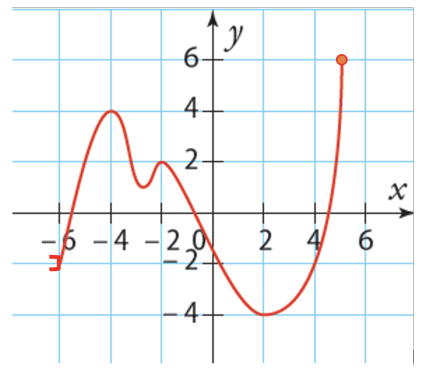
\includegraphics[scale=.6]{Ch 2/Exercice}
\end{center}
\end{minipage}
\end{Exercice}



\begin{Exercice}
On considère le tableau de variations d'une fonction \( f \) ci-dessous. 
\begin{center}
\begin{tikzpicture}[scale=.9]
   \tkzTabInit{$x$ / 1 ,  Variations de $f $ / 2}{$-7$, $ 0 $ , $ 3 $, $6$}
   \tkzTabVar{+/ 3, -/ -2,+/0, -/ -5}

\end{tikzpicture}
\end{center}
Dans cet exercice, on répondra aux questions quand cela est possible. Si le tableau ne permet pas de répondre à une question, on écrira : "on ne peut pas savoir".
\begin{enumerate}

\item Donner l'ensemble de définition de \( f \).
\item Donner le signe des nombres suivants : \( f(-6) \), \( f(2) \), \( f(5) \).
\item Comparer les nombres suivants :

\begin{enumerate}

\item \( f(5) \) ... \( f(-4) \)
\item \( f(3) \) ... \( f(2) \)
\item \( f(5) \) ... \( f(6) \)
\item \( f(3) \) ... \( 4 \)
\end{enumerate}
\item Sur quel(s) intervalle(s) la fonction est-elle décroissante ?
\item Pour quelle valeur de \( x \) la fonction atteint-elle son minimum ? Quelle est la valeur de ce minimum ?
\item Quel est le maximum de la fonction ? Pour quelle valeur de \( x \) est-il atteint ?
\item Donner un encadrement de \( f(5) \).
\end{enumerate}
\end{Exercice}

\newpage

\begin{Exercice}
On considère le tableau de variations d'une fonction \( f \) ci-dessous. 
\begin{center}
\begin{tikzpicture}[scale=.9]
   \tkzTabInit{$x$ / 1 ,  Variations de $f $ / 2}{$-8$, $ -4 $ , $ 0 $, $2$,$ 7 $}
   \tkzTabVar{+/ 6, -/ -2,+/4, -/ 1,+/7}

\end{tikzpicture}
\end{center}

Dans cet exercice, on répondra aux questions quand cela est possible. Si le tableau ne permet pas de répondre à une question, on écrira : "on ne peut pas savoir".
\begin{enumerate}

\item Donner l'ensemble de définition de \( f \).
\item Donner le signe des nombres suivants : \( f(-6) \), \( f(1) \), \( f(5) \).
\item Comparer les nombres suivants :
\begin{enumerate}

\item \( f(5) \) ... \( f(-3) \)
\item \( f(3) \) ... \( f(2) \)
\item \( f(5) \) ... \( f(6) \)
\item \( f(3) \) ... \( 4 \)
   \end{enumerate}
\item Sur quel(s) intervalle(s) la fonction est-elle décroissante ?
\item Pour quelle valeur de \( x \) la fonction atteint-elle son minimum ?Quelle est la valeur de ce minimum ?
\item Quel est le maximum de la fonction ? Pour quelle valeur de \( x \) est-il atteint ?
\item Donner un encadrement de \( f(5) \).
\end{enumerate}
\end{Exercice}

\begin{Exercice}
On a mesuré la température dans une ville tout au long de la journée. La température en fonction de l’heure de la journée est représentée sur le graphique ci-dessous.
\begin{center}
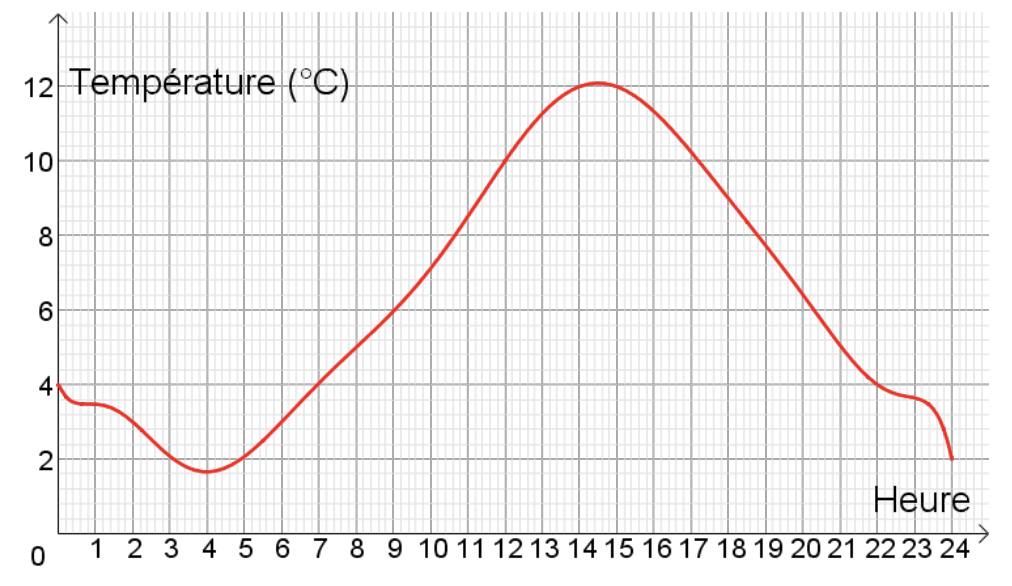
\includegraphics[scale=.7]{Ch 2/Exercice21}
\end{center}

\begin{enumerate}
    \item Quelle température faisait-il à midi ?
    \item À quelle heure de la journée la température est-elle passée au-dessus de 6°C ?
    \item Pour une heure de la journée \( h \), on note \( T(h) \) la température à cette heure de la journée. On définit ainsi une fonction \( T \) sur l’intervalle \([0; 24[\).
    \begin{enumerate}
        \item Traduire les égalités \( T(6) = 3 \) et \( T(18) = 9 \) dans le contexte de l’exercice.
        \item Déterminer graphiquement \( T(14) \).
        \item On souhaite résoudre graphiquement l’inéquation \( T(h) > 4 \). Traduire cette inéquation par une phrase dans le contexte de l’exercice puis résoudre cette inéquation.
    \end{enumerate}
\end{enumerate}
\end{Exercice}



\begin{Exercice}
\begin{minipage}[c]{0.5\textwidth}
Pour traiter un patient, un médecin procède à l'injection intramusculaire d'une substance médicamenteuse au temps \(t = 0\), \(t\) étant exprimé en heures. Pour tout réel de \([0 : 6]\), la concentration du principe actif en mg.L\(^{-1}\), \(t\) heures après l'injection est donnée par la fonction \(c\) définie par
\[ c(t) = t^3 - 12t^2 + 36t \]
Le médicament est efficace lorsque la concentration du principe actif est supérieure ou égale à 25 mg.L\(^{-1}\). La courbe représentative de la fonction \(c\) est donnée ci-dessous.
\end{minipage} \hfill \begin{minipage}[c]{0.5\textwidth}
\begin{center}
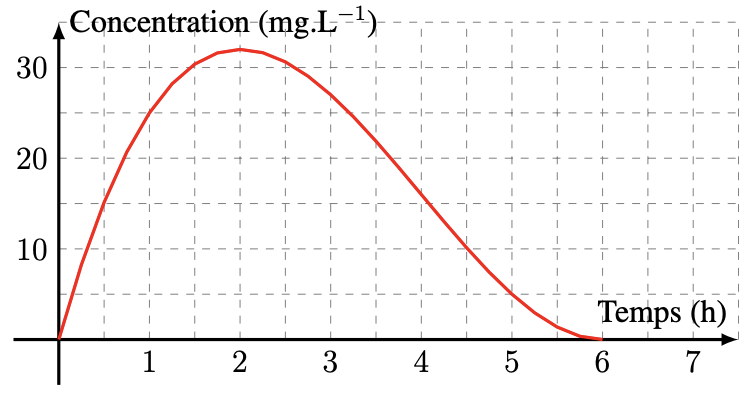
\includegraphics[scale=.5]{Ch 2/Exercice23}
\end{center}
\end{minipage}
\begin{enumerate}
    \item Quelle est la concentration du principe actif après 30 minutes ? On utilisera le graphique ET le calcul.
    \item À partir de quel temps n’y a-t-il plus de principe actif ?
    \item Justifier que pour tout réel \(t\), \(c(t) = t(t - 6)^2\).
    \item Vérifier le résultat de la question 2 par le calcul.
    \item Durant quelle période le médicament est-il efficace ?
\end{enumerate}
\end{Exercice}

\subsection*{Parité}


\begin{Exercice}
Soit \( f \) la fonction définie pour tout réel \( x \) par \( f(x) = 2x^2 + 3x - 1 \)
\begin{enumerate}
    \item Calculer \( f(1) \) et \( f(-1) \)
    \item La fonction \( f \) est-elle paire ? impaire ?
\end{enumerate}
\end{Exercice}

\begin{Exercice}
Soit \( f \) la fonction définie pour tout réel \( x \) par \( f(x) = x^2 - 7 \)
\begin{enumerate}
    \item Calculer \( f(2) \) et \( f(-2) \). La fonction \( f \) est-elle impaire ?
    \item Soit \( x \) un réel. Montrer que \( f(-x) = f(x) \). Qu'en déduit-on sur la fonction \( f \) ?
\end{enumerate}
\end{Exercice}



\begin{Exercice}
Déterminer la parité des fonctions suivantes, définies sur le domaine de définition associé :
\vspace{-0.5cm}
\begin{multicols}{3}
\begin{enumerate}
    \item \( f : x \mapsto x^3 - 1 \) sur \( \mathbb{R} \)
    \item \( g : x \mapsto x^2 + \frac{1}{x^2} \) sur \( \mathbb{R} \setminus \{0\} \)
    \item \( h : x \mapsto x^2 + 1 \) sur \([-3; 5]\)
    \item \( i : x \mapsto 3x + 2 \) sur \( \mathbb{R} \)
    \item \( j : x \mapsto \sqrt{x^2 + 3} \) sur \( \mathbb{R} \)
    \item \( k : x \mapsto 2x^3 - 4x \) sur \( \mathbb{R} \)
\end{enumerate}
\end{multicols}
\end{Exercice}

\newpage

\begin{Exercice}
Parmi les représentations graphiques suivantes, lesquelles sont la courbe d’une fonction paire ? D’une fonction impaire ?
\begin{center}
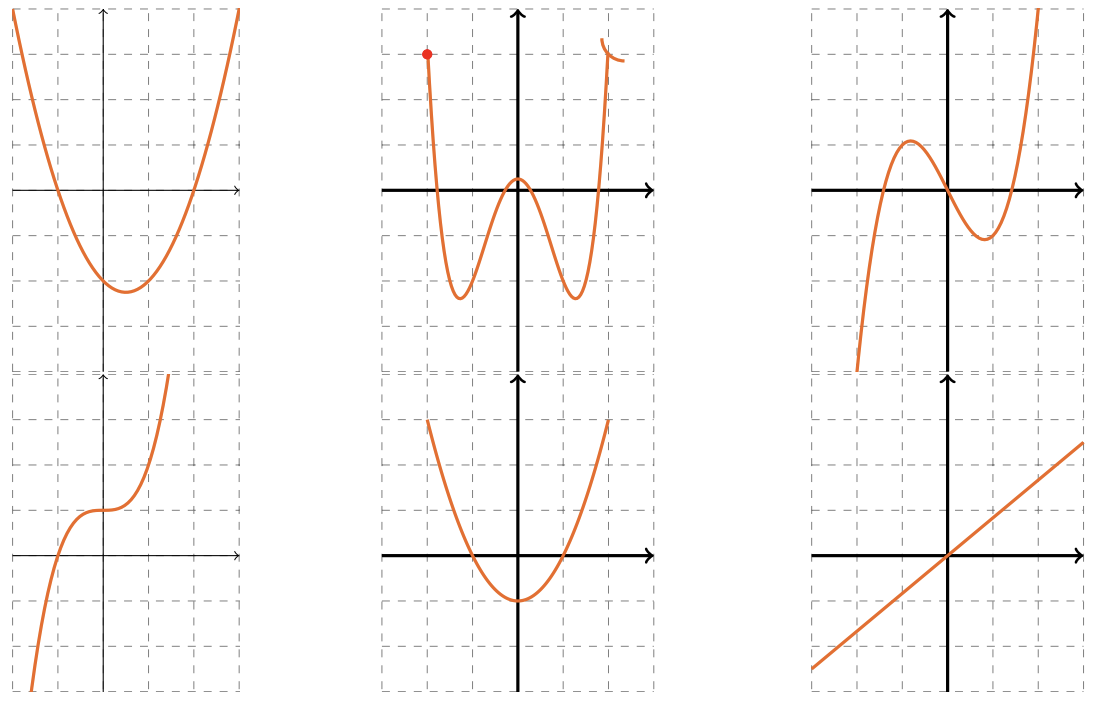
\includegraphics[scale=.8]{Ch 2/Exercice27}
\end{center}
\end{Exercice}

\begin{Exercice}
\leavevmode\vspace{-\baselineskip}
\begin{enumerate}
\item Soit \( f \) une fonction paire. Compléter le tableau de variations et de signes de la fonction ci-dessous.
\begin{center}
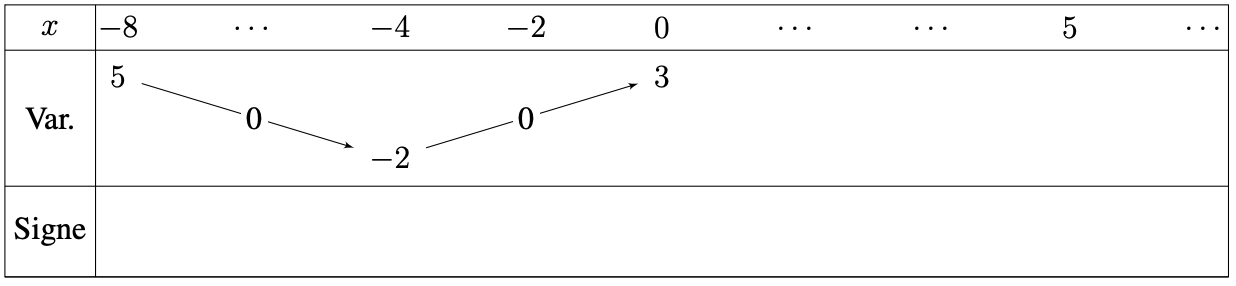
\includegraphics[scale=.5]{Ch 2/Exercice28}
\end{center}
\begin{center}

\end{center}

\item Soit \( g \) une fonction impaire. Compléter le tableau de variations et de signes de la fonction ci-dessous.
\begin{center}
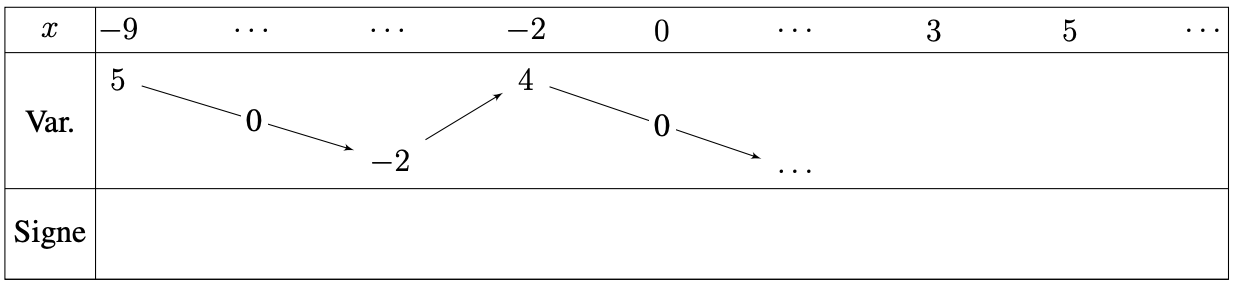
\includegraphics[scale=.5]{Ch 2/Exercice29}
\end{center}
\begin{center}

\end{center}
\end{enumerate}
\end{Exercice}
}
